\documentclass[10pt]{article}
\usepackage[verbose, a4paper, hmargin=2.5cm, vmargin=2.5cm]{geometry}

\usepackage{fontspec}
\usepackage{ctex}
\usepackage{paratype}

\usepackage{amsmath}
\usepackage{amssymb}
\usepackage{amsfonts}
\usepackage{esint}
\usepackage{stmaryrd}

\usepackage[mathbf=sym]{unicode-math}
\setmainfont{STIX Two Text}
\setmathfont{STIX Two Math}

\setsansfont{Arial}
\setmonofont{Courier New}

\usepackage{makecell}
\usepackage{wasysym}
\usepackage{pifont}
\usepackage[export]{adjustbox}
\usepackage{graphicx}
\usepackage{mdframed}
\usepackage{booktabs,array,multirow}
\usepackage{tabularx}
\usepackage{hyperref}
\hypersetup{colorlinks=true, linkcolor=blue, filecolor=magenta, urlcolor=cyan,}
\urlstyle{same}
\usepackage[most]{tcolorbox}
\definecolor{mygray}{RGB}{240,240,240}
\tcbset{
  colback=mygray,
  boxrule=0pt,
}
\graphicspath{ {./images/} }
\newcommand{\HRule}{\begin{center}\rule{0.9\linewidth}{0.2mm}\end{center}}
\newcommand{\customfootnote}[1]{
  \let\thefootnote\relax\footnotetext{#1}
}
\newcommand{\lt}{\mathrel{<}}
\newcommand{\gt}{\mathrel{>}}
\newcommand*\circled[1]{\tikz[baseline=(char.base)]{\node[shape=circle,draw,inner sep=1.5pt] (char) {\small #1};}}
\setcounter{MaxMatrixCols}{256}
\begin{document}
\section*{25 秋}

\section*{一、填空题}

1. 已知全集 \(U = \{ x \mid  2 \leq  x \leq  5,x \in  R\}\) ，集合 \(A = \{ x \mid  2 \leq  x < 4,x \in  R\}\) ，则 \(\bar{A} =\) \_\_\_\_\_.

2. 不等式 \(\frac{x - 1}{x - 3} < 0\) 的解集为\_\_\_\_\_.

3. 己知等差数列 \(\left\{  {a}_{n}\right\}\) 的首项 \({a}_{1} =  - 3\) ，公差 \(d = 2\) ，则该数列的前 6 项和为\_\_\_\_\_.

4. 在二项式 \({\left( 2x - 1\right) }^{5}\) 的展开式中， \({x}^{3}\) 的系数为\_\_\_\_\_.

5. 函数 \(y = \cos x\) 在 \(\left\lbrack  {-\frac{\pi }{2},\frac{\pi }{4}}\right\rbrack\) 上的值域为\_\_\_\_\_.

6. 已知随机变量 \(X\) 的分布为 \(\left( \begin{matrix} 5 & 6 & 7 \\  {0.2} & {0.3} & {0.5} \end{matrix}\right)\) ,则期望 \(E\left\lbrack  X\right\rbrack   =\) \_\_\_\_\_.

7. 如图，在正四棱柱 \({ABCD} - {A}_{1}{B}_{1}{C}_{1}{D}_{1}\) 中， \({BD} = {4\sqrt{2}}\) ， \({D{B}_{1}} = 9\) ，则该正四棱柱的体积为

\begin{center}
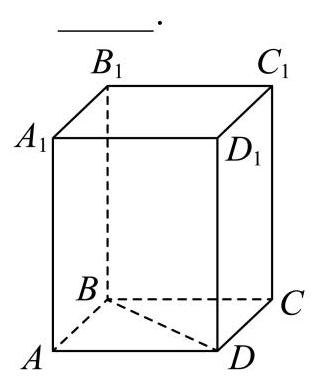
\includegraphics[max width=0.2\textwidth]{images/bo_d6dcisv7aajc739b5agg_1_257_278_315_381_0.jpg}
\end{center}
\hspace*{3em} 

8. 设 \(a,b > 0,a + \frac{1}{b} = 1\) ，则 \(b + \frac{1}{a}\) 的最小值为\_\_\_\_\_.

9.4 个家长和 2 个儿童去爬山, 6 个人需要排成一条队列, 要求队列的头和尾均是家长, 则不同的排列个数有\_\_\_\_\_种.

10. 已知复数 \(z\) 满足 \({z}^{2} = {\left( \bar{z}\right) }^{2},\;\left| z\right|  \leq  1\) ，则 \(\left| {z - 2 - 3\mathrm{i}}\right|\) 的最小值是\_\_\_\_\_.

11. 小申同学观察发现, 生活中有些时候影子可以完全投射在斜面上. 某斜面上有两根长为 1 米的垂直于水平面放置的杆子，与斜面的接触点分别为 \(A\) 、 \(B\) ，它们在阳光的照射下呈现出影子，阳光可视为平行光:其中一根杆子的影子在水平面上，长度为 0.4 米；另一根杆子的影子完全在斜面上，长度为 0.45 米. 则斜面的底角 \(\theta  =\) \_\_\_\_\_. (结果用角度制表示， 精确到 \(\left. {0.{01}^{ \circ  }}\right)\)

\begin{center}
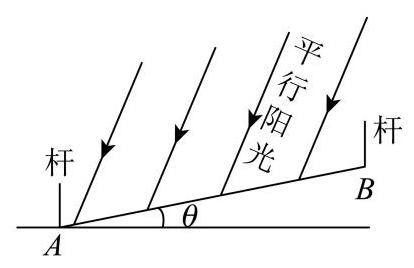
\includegraphics[max width=0.3\textwidth]{images/bo_d6dcisv7aajc739b5agg_2_254_215_414_268_0.jpg}
\end{center}
\hspace*{3em} 

12. 已知 \(f\left( x\right)  = \left\{  \begin{matrix} 1, & x > 0 \\  0, & x = 0 \\   - 1, & x < 0 \end{matrix}\right.\) , \(\overrightarrow{a}\text{ 、 }\overrightarrow{b}\text{ 、 }\overrightarrow{c}\) 是平面内三个不同的单位向量. 若 \(f\left( {\overrightarrow{a} \cdot  \overrightarrow{b}}\right)  + f\left( {\overrightarrow{b} \cdot  \overrightarrow{c}}\right)  + \; f\left( {\overrightarrow{c} \cdot  \overrightarrow{a}}\right)  = 0\) ，则 \(\left| {\overrightarrow{a} + \overrightarrow{b} + \overrightarrow{c}}\right|\) 的取值范围是\_\_\_\_\_.

\section*{二、单选题}

13. 已知事件 \(A\text{ 、 }B\) 相互独立,事件 \(A\) 发生的概率为 \(P\left( A\right)  = \frac{1}{2}\) ,事件 \(B\) 发生的概率为 \(P\left( B\right) \; = \frac{1}{2}\) ,则事件 \(A \cap  B\) 发生的概率 \(P\left( {A \cap  B}\right)\) 为 ( )

A. \(\frac{1}{8}\) B. \(\frac{1}{4}\) C. \(\frac{1}{2}\) D. 0

14. 设 \(a > 0,s \in  R\) . 下列各项中,能推出 \({a}^{s} > a\) 的一项是 ( )

A. \(a > 1\) ,且 \(s > 0\) B. \(a > 1\) ,且 \(s < 0\)

C. \(0 < a < 1\) ,且 \(s > 0\) D. \(0 < a < 1\) ，且 \(s < 0\)

15. 已知 \(A\left( {0,1}\right) ,B\left( {1,2}\right) ,C\) 在 \(\Gamma  : {x}^{2} - {y}^{2} = 1\left( {x \geq  1,y \geq  0}\right)\) 上,则 \(\bigtriangleup {ABC}\) 的面积 ( )

A. 有最大值，但没有最小值 B. 没有最大值，但有最小值

C. 既有最大值, 也有最小值 D. 既没有最大值, 也没有最小值

16. 已知数列 \(\left\{  {a}_{n}\right\}  \text{ 、 }\left\{  {b}_{n}\right\}  \text{ 、 }\left\{  {c}_{n}\right\}\) 的通项公式分别为 \({a}_{n} = {10n} - 9,{b}_{n} = {2}^{n}\text{ 、 },{c}_{n} = \lambda {a}_{n} + \; \left( {1 - \lambda }\right) {b}_{n}\) . 若对任意的 \(\lambda  \in  \left\lbrack  {0,1}\right\rbrack\) ， \({a}_{n}\) 、 \({b}_{n}\) 、 \({c}_{n}\) 的值均能构成三角形，则满足条件的正整数 \(n\) 有 ( )

A. 4 个 B. 3 个 C. 1 个 D. 无数个

\section*{三、解答题}

17. 2024 年巴黎奥运会, 中国获得了男子 4 × 100 米混合泳接力金牌. 以下是历届奥运会男子 4 0 天)100 米混合泳接力项目冠军成绩记录(单位:秒)，数据按照升序排列.

\begin{center}
\adjustbox{max width=\textwidth}{
\begin{tabular}{|c|c|c|c|c|}
\hline
206.78 & 207.46 & 207.95 & 209.34 & 209.35 \\
\cline{1-5}
210.68 & 213.73 & 214.84 & 216.93 & 216.93 \\
\cline{1-5}
\hline
\end{tabular}
}
\end{center}

(1)求这组数据的极差与中位数；

(2)从这 10 个数据中任选 3 个，求恰有 2 个数据在 211 以上的概率；

(3)若比赛成绩 \(y\) 关于年份 \(x\) 的回归方程为 \(y =  - {0.311x} + \widehat{b}\) ，年份 \(x\) 的平均数为 2006，预测 2028 年冠军队的成绩 (精确到 0.01 秒).

18. 如图, \(P\) 是圆锥的顶点, \(O\) 是底面圆心, \({AB}\) 是底面直径,且 \({AB} = 2\) .

\begin{center}
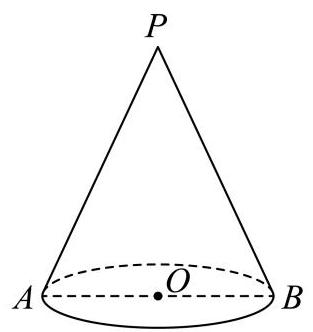
\includegraphics[max width=0.2\textwidth]{images/bo_d6dcisv7aajc739b5agg_4_259_218_313_332_0.jpg}
\end{center}
\hspace*{3em} 

(1)若直线 \({PA}\) 与圆锥底面的所成角为 \(\frac{\pi }{3}\) ，求圆锥的侧面积；

(2)已知 \(Q\) 是母线 \({PA}\) 的中点，点 \(C\) 、 \(D\) 在底面圆周上，且弧 \({AC}\) 的长为 \(\frac{\pi }{3}\) ， \({CD}//{AB}\) . 设点 \(M\) 在线段 \({OC}\) 上，证明:直线 \({QM}//\) 平面 \({PBD}\) .

19. 已知 \(f\left( x\right)  = {x}^{2} - \left( {m + 2}\right) x + m\ln x,\;m \in  R\) .

(1)若 \(f\left( 1\right)  = 0\) ，求不等式 \(f\left( x\right)  \leq  {x}^{2} - 1\) 的解集；

(2)若函数 \(y = f\left( x\right)\) 满足在 \(\left( {0, + \infty }\right)\) 上存在极大值，求 \(m\) 的取值范围；

20. 已知椭圆 \(\Gamma  : \frac{{x}^{2}}{{a}^{2}} + \frac{{y}^{2}}{5} = 1\left( {a > \sqrt{5}}\right) ,M\left( {0,m}\right) \left( {m0}\right) ,A\) 是 \(\Gamma\) 的右顶点.

(1)若 \(\Gamma\) 的焦点 \(\left( {2,0}\right)\) ，求离心率 \(\mathrm{e}\) ；

(2)若 \(a = 4\) ，且 \(\Gamma\) 上存在一点 \(P\) ，满足 \(\overrightarrow{PA} = 2\overrightarrow{MP}\) ，求 \(m\) ；

(3)已知 \({AM}\) 的中垂线 \(l\) 的斜率为 \(2,l\) 与 \(\Gamma\) 交于 \(C\) 、 \(D\) 两点， \(\angle {CMD}\) 为钝角，求 \(a\) 的取值范围.

21. 已知函数 \(y = f\left( x\right)\) 的定义域为 \(R\) . 对于正实数 \(a\) ,定义集合 \({M}_{a} = \{ x \mid  f\left( {x + a}\right)  = f\left( x\right) \}\) .

(1) 若 \(f\left( x\right)  = \sin x\) ,判断 \(\frac{\pi }{3}\) 是否是 \({M}_{\pi }\) 中的元素,请说明理由;

(2)若 \(f\left( x\right)  = \left\{  {\begin{array}{ll} x + 2, & x < 0 \\  \sqrt{x}, & x \geq  0 \end{array},\;{M}_{a} \neq  \varnothing }\right.\) ，求 \(a\) 的取值范围；

(3)若 \(y = f\left( x\right)\) 是偶函数，当 \(x \in  (0,1\rbrack\) 时， \(f\left( x\right)  = 1 - x\) ，且对任意 \(a \in  \left( {0,2}\right)\) ，均有 \({M}_{a} \subseteq  {M}_{2}\) . 写出 \(y = f\left( x\right)\) ， \(x \in  \left( {1,2}\right)\) 解析式，并证明:对任意实数 \(c\) ，函数 \(y = f\left( x\right)  - c\) 在 \(\left\lbrack  {-3,3}\right\rbrack\) 上至多有 9 个零点.

\section*{25 春}

一、填空题

1. 已知集合 \(A = \{ x \mid  x > 0\} ,B = \{  - 1,0,1,2\}\) ，则 \(A \cap  B\) 等于\_\_\_\_\_.

2. 不等式 \(\frac{x}{x - 1} < 0\) 的解集为\_\_\_\_\_.

3. 已知复数 \(z = \frac{2 + i}{i}\) ( \(\mathrm{i}\) 是虚数单位),则 \(\left| z\right|  =\) \_\_\_\_\_.

4. 已知 \(\overrightarrow{a} = \left( {2,1}\right) ,\overrightarrow{b} = \left( {1,x}\right)\) ,若 \(\overrightarrow{a}//\overrightarrow{b}\) ,则 \(x =\) \_\_\_\_\_.

5. 已知 \(\tan \alpha  = 1\) ，则 \(\cos \left( {\alpha  + \frac{\pi }{4}}\right)  =\) \_\_\_\_\_.

6. 若 \({\left( x + \frac{a}{x}\right) }^{6}\) 的展开式中的常数项为 20，则 \(a =\) \_\_\_\_\_.

7. 已知 \(\left\{  {a}_{n}\right\}\) 是首项为 1、公差为 1 的等差数列， \(\left\{  {b}_{n}\right\}\) 是首项为 1、公比为 \(q\left( {q0}\right)\) 的等比数列. 若数列 \(\left\{  {{a}_{n} \cdot  {b}_{n}}\right\}\) 的前三项和为 2,则 \(q =\) \_\_\_\_\_.

8. 关于 \(x\) 的方程 \(\left| {x - 1}\right|  + \left| {\pi  - x}\right|  = \pi  - 1\) 的解集为\_\_\_\_\_.

9. 已知 \(P\) 是一个圆锥的顶点， \({PA}\) 是母线， \({PA} = 2\) ，该圆锥的底面半径是 1 . \(B\) 、 \(C\) 分别在圆锥的底面上，则异面直线 \({PA}\) 与 \({BC}\) 所成角的最小值为\_\_\_\_\_.

10. 已知双曲线 \(\frac{{x}^{2}}{{a}^{2}} - \frac{{y}^{2}}{6 - {a}^{2}} = 1\left( {a > 0}\right)\) 的左、右焦点分别为 \({F}_{1}\text{ 、 }{F}_{2}\) . 通过 \({F}_{2}\) 且倾斜角为 \(\frac{\pi }{3}\) 的直线与双曲线交于第一象限的点 \(A\) ,延长 \(A{F}_{2}\) 至 \(B\) 使得 \({AB} = A{F}_{1}\) . 若 \(\bigtriangleup B{F}_{1}{F}_{2}\) 的面积为 \(3\sqrt{6}\) ，则 \(a\) 的值为\_\_\_\_\_.

11. 如图所示,正方形 \({ABCD}\) 是一块边长为 4 的工程用料,阴影部分所示是被腐蚀的区域,其余部分完好,曲线 \({MN}\) 为以 \({AD}\) 为对称轴的抛物线的一部分, \({DM} = {DN} = 3\) . 工人师傅现要从完好的部分中截取一块矩形原料 \({BQPR}\) ，当其面积有最大值时， \({AQ}\) 的长为\_\_\_\_\_.

\begin{center}
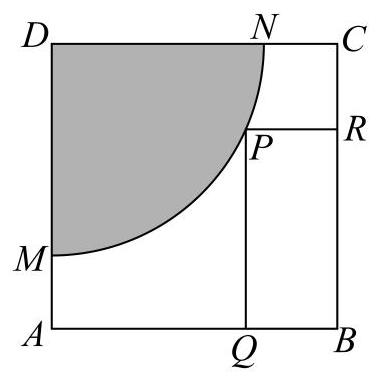
\includegraphics[max width=0.2\textwidth]{images/bo_d6dcisv7aajc739b5agg_7_255_548_377_376_0.jpg}
\end{center}
\hspace*{3em} 

12. 在平面中, \({\overrightarrow{\mathrm{e}}}_{1}\) 和 \({\overrightarrow{\mathrm{e}}}_{2}\) 是互相垂直的单位向量,向量 \(\overrightarrow{a}\) 满足 \(\left| {\overrightarrow{a} - 4{\overrightarrow{\mathrm{e}}}_{1}}\right|  = 2\) ,向量 \(\overrightarrow{b}\) 满足 \(\left| {\overrightarrow{b} - 6{\overrightarrow{\mathrm{e}}}_{2}}\right| \; = 1\) ，求 \(\overrightarrow{b}\) 在 \(\overrightarrow{a}\) 方向上的数量投影的最大值\_\_\_\_\_.

二、选择题

13. 如图, \({ABCD} - {A}_{1}{B}_{1}{C}_{1}{D}_{1}\) 是正四棱台,则下列各组直线中属于异面直线的是 ().

\begin{center}
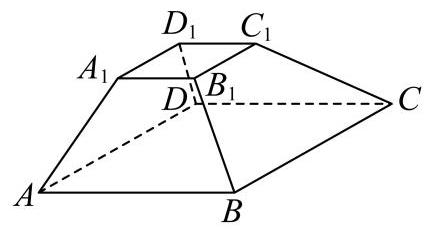
\includegraphics[max width=0.3\textwidth]{images/bo_d6dcisv7aajc739b5agg_7_256_1606_428_229_0.jpg}
\end{center}
\hspace*{3em} 

A. \({AB}\) 和 \({C}_{1}{D}_{1}\) ; B. \(A{A}_{1}\) 和 \(C{C}_{1}\) ; C. \(B{D}_{1}\) 和 \({B}_{1}D\) ; D. \({A}_{1}{D}_{1}\) 和 \({AB}\) .

14. 幂函数 \(y = {x}^{a}\) 在 \(\left( {0, + \infty }\right)\) 上是严格减函数,且经过 \(\left( {-1, - 1}\right)\) ,则 \(a\) 的值可能是 ( ).

A. \(- \frac{2}{3}\) B. \(- \frac{1}{3}\) C. \(\frac{1}{3}\) D. 3

15. 有一四边形 \({ABCD}\) ,对于其四边 \({AB}\text{ 、 }{BC}\text{ 、 }{CD}\text{ 、 }{DA}\) ,按顺序分别抛掷一枚质量均匀的硬币: 如硬币正面朝上，则将其擦去；如硬币反面朝上，则不擦去. 最后，以 \(A\) 为起点沿着尚未擦去的边出发，可以到达 \(C\) 点的概率为 ( ).

A. \(\frac{1}{2}\) B. \(\frac{7}{16}\) C. \(\frac{1}{4}\) D. \(\frac{3}{16}\)

16. 已知 \(a \in  R\) ,不等式 \(\left\lbrack  {\tan \left( {\frac{\pi }{6}x}\right)  - a}\right\rbrack  \left\lbrack  {\tan \left( {\frac{\pi }{6}x}\right)  - a - 1}\right\rbrack   < 0\) 在 \(\left( {0,{2025}}\right)\) 中的整数解有 \(m\) 个. 关于 \(m\) 的个数,以下不可能的是 ( ).

A. 0 B. 338 C. 674 D. 1012

三、解答题

17. 在三棱锥 \(P - {ABC}\) 中,平面 \({PAC} \bot\) 平面 \({ABC},{PA} = {AC} = {CP} = 2,{AB} = {BC} = \sqrt{2}\) ,

\begin{center}
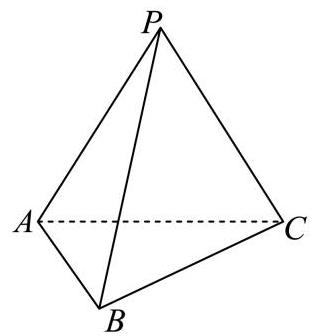
\includegraphics[max width=0.2\textwidth]{images/bo_d6dcisv7aajc739b5agg_8_258_1586_317_336_0.jpg}
\end{center}
\hspace*{3em} 

(1)若 \(O\) 是棱 \({AC}\) 的中点，证明: \({BO}\bot\) 平面 \({PAC}\) ，并求三棱锥 \(B - {OPA}\) 的体积；

(2) 求二面角 \(B - {PC} - A\) 的大小.

18. 在 \(\bigtriangleup {ABC}\) 中,角 \(A\text{ 、 }B\text{ 、 }C\) 所对的边分别为 \(a\text{ 、 }b\text{ 、 }c\) ,且 \(c = 5\) .

(1) 若 \(\frac{a}{4b} = \frac{\sin B}{\sin A},C = \frac{\pi }{2}\) ,求 \(a\) ;

(2)若 \({ab} = {20}\) ，求 \(\bigtriangleup  {ABC}\) 的面积的最大值.

19. 甲、乙是两个体育社团的小组. 如下是两组组员身高的茎叶图 (单位:厘米)，以身高的百位数和十位数作为 “茎” 排列在中间、个位数作为 “叶” 分列在两边.

\begin{center}
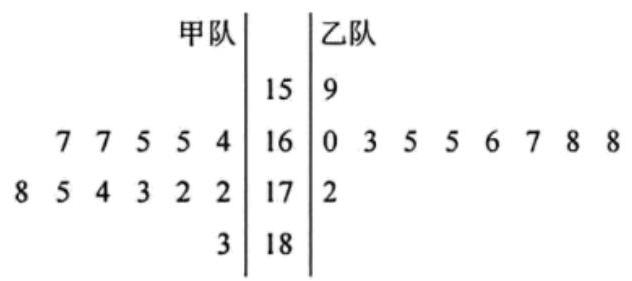
\includegraphics[max width=0.4\textwidth]{images/bo_d6dcisv7aajc739b5agg_9_263_936_632_281_0.jpg}
\end{center}
\hspace*{3em} 

甲、乙两小组组员身高分布茎叶图

(1)求甲、乙两组组员身高的第 60 百分位数；

(2)从甲、乙两组各选取一个组员，求两人身高均在 170 厘米以上的概率；

(3)为使两组人数相同，从甲组中调派一个队员到乙组. 是否存在甲组的一个组员，将他调派至乙组后, 甲、乙两组的平均身高都增大?

20. 在平面直角坐标系中,已知曲线 \(\Gamma  : \frac{{x}^{2}}{4} + {y}^{2} = 1\left( {y \geq  0}\right)\) ,点 \(P\text{ 、 }Q\) 分别为 \(\Gamma\) 上不同的两点, \(T\left( {t,0}\right)\) .

\begin{center}
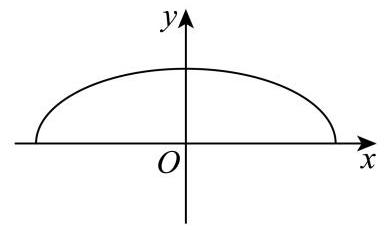
\includegraphics[max width=0.3\textwidth]{images/bo_d6dcisv7aajc739b5agg_9_256_1830_386_230_0.jpg}
\end{center}
\hspace*{3em} 

(1) 求 \(\Gamma\) 所在椭圆的离心率;

( 2 )若 \(T\left( {1,0}\right)\) ， \(Q\) 在 \(y\) 轴上，若 \(T\) 到直线 \({PQ}\) 的距离为 \(\frac{\sqrt{5}}{5}\) ，求 \(P\) 的坐标；

(3)是否存在 \(t\) ，使得 \(\bigtriangleup  {TPQ}\) 是以 \(T\) 为直角顶点的等腰直角三角形？若存在，求 \(t\) 的取值范围； 若不存在, 请说明理由.

21. 已知函数 \(y = f\left( x\right)\) 的定义域是 \(D\) . 对于 \(t \in  D\) ,定义集合 \({S}_{f\left( t\right) } = \{ x \mid  f\left( x\right)  \geq  f\left( t\right) \}\) .

(1) \(f\left( x\right)  = {\log }_{2}x\) ，求 \({S}_{f\left( {16}\right) }\) ；

(2)对于集合 \(A\) ，若对任意 \(x \in  A\) 都有 \(- x \in  A\) ，则称 \(A\) 是对称集. 若 \(D\) 是对称集，证明: “函数 \(y = f\left( x\right)\) 是偶函数” 的充要条件是 “对任意 \(t \in  D,{S}_{f\left( t\right) }\) 是对称集”;

(3) 若 \(x \in  R,f\left( x\right)  = {\mathrm{e}}^{x} - \frac{1}{2}m{x}^{2}\) . 求 \(m\) 的取值范围,使得对于任意 \({t}_{1} < {t}_{2} \in  D\) ,都有 \({S}_{f\left( {t}_{2}\right) } \subseteq \; {S}_{f\left( {t}_{1}\right) }\) .

24 秋

1. 设全集 \(U = \{ 1,2,3,4,5\}\) ，集合 \(A = \{ 2,4\}\) ，则 \(\bar{A} =\) \_\_\_\_\_.

2. 已知 \(f\left( x\right)  = \left\{  \begin{array}{ll} \sqrt{x}, & x > 0 \\  1, & x \leq  0 \end{array}\right.\) 则 \(f\left( 3\right)  =\) \_\_\_\_\_.

3. 已知 \(x \in  R\) ，则不等式 \({x}^{2} - {2x} - 3 < 0\) 的解集为\_\_\_\_\_.

4. 已知 \(k \in  R\) ， \(\overrightarrow{a} = \left( {2,5}\right)\) ， \(\overrightarrow{b} = \left( {6,k}\right)\) ，且 \(\overrightarrow{a}//\overrightarrow{b}\) ，则 \(k\) 的值为\_\_\_\_\_.

5. 已知 \(f\left( x\right)  = {x}^{3} + a\) 为奇函数，则 \(a =\) \_\_\_\_\_.

6. 在 \({\left( x + 1\right) }^{n}\) 的二项展开式中，若各项系数和为 32，则 \({x}^{2}\) 项的系数为\_\_\_\_\_.

7. 已知抛物线 \({y}^{2} = {4x}\) 上有一点 \(P\) 到准线的距离为 9，那么点 \(P\) 到 \(x\) 轴的距离为\_\_\_\_\_.

8. 某校举办科学竞技比赛,有 \(A\text{ 、 }B\text{ 、 }{C3}\) 种题库, \(A\) 题库有 5000 道题, \(B\) 题库有 4000 道题, \(C\) 题库有 3000 道题. 小申已完成所有题,他 \(A\) 题库的正确率是 \({0.92},B\) 题库的正确率是 0.86， \(C\) 题库的正确率是 0.72 . 现他从所有的题中随机选一题，正确率是\_\_\_\_\_.

9. 已知虚数 \(z\) ,其实部为 1,且 \(z + \frac{2}{z} = m\left( {m \in  R}\right)\) ,则实数 \(m\) 为\_\_\_\_\_.

10. 设集合 \(A\) 中的元素皆为无重复数字的三位正整数，且元素中任意两者之积皆为偶数，则集合中元素个数的最大值为\_\_\_\_\_.

11. 如图，某海域内有一小岛 \(C\) ，观测点 \(B\) ， \(D\) 分别在小岛 \(C\) 的正北方向和正东方向，且 \({CB} \; = {CD}\) ，观测到海域内有一小船 \(A\) 满足 \(\angle {BAC} = {16.5}^{ \circ  }\) ， \(\angle {DAC} = {37}^{ \circ  }\) ，则 \(\angle {BCA} =\) \_\_\_\_\_. (精确到 \({0.1}^{ \circ  }\) 度)

\begin{center}
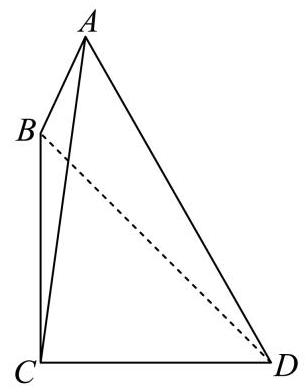
\includegraphics[max width=0.2\textwidth]{images/bo_d6dcisv7aajc739b5agg_12_255_901_307_392_0.jpg}
\end{center}
\hspace*{3em} 

12. 无穷等比数列 \(\left\{  {a}_{n}\right\}\) 满足首项 \({a}_{1} > 0,q > 1\) ,记 \({I}_{n} = \left\{  {x - y \mid  x,y \in  \left\lbrack  {{a}_{1},{a}_{2}}\right\rbrack   \cup  \left\lbrack  {{a}_{n},{a}_{n + 1}}\right\rbrack  }\right\}\) ,若对任意正整数 \(n\) ，集合 \({I}_{n}\) 是闭区间，则 \(q\) 的取值范围是\_\_\_\_\_.

二、选择题 (本大题共 4 题,满分 18 分,第 13-14 题每题 4 分,第 \({15} - {16}\) 题每题 5 分)

13. 已知气候温度和海水表层温度相关，且相关系数为正数，对此描述正确的是 ( )

A. 气候温度高, 海水表层温度就高

B. 气候温度高，海水表层温度就低

C. 随着气候温度由低到高，海水表层温度呈上升趋势

D. 随着气候温度由低到高，海水表层温度呈下降趋势

14. 下列函数 \(f\left( x\right)\) 的最小正周期是 \({2\pi }\) 的是 ( )

A. \(f\left( x\right)  = \sin x + \cos x\) B. \(f\left( x\right)  = \sin x\cos x\)

C. \(f\left( x\right)  = {\sin }^{2}x + {\cos }^{2}x\) D. \(f\left( x\right)  = {\sin }^{2}x - {\cos }^{2}x\)

15. 定义一个集合 \(\Omega\) ,集合中的元素是空间内的点集,任取 \({P}_{1},{P}_{2},{P}_{3} \in  \Omega\) ,存在不全为 0 的实数 \({\lambda }_{1},{\lambda }_{2},{\lambda }_{3}\) ,使得 \({\lambda }_{1}\overrightarrow{O{P}_{1}} + {\lambda }_{2}\overrightarrow{O{P}_{2}} + {\lambda }_{3}\overrightarrow{O{P}_{3}} = \overrightarrow{0}\) . 已知 \(\left( {1,0,0}\right)  \in  \Omega\) ,则 \(\left( {0,0,1}\right)  \notin  \Omega\) 的充分条件是 ( )

A. \(\left( {0,0,0}\right)  \in  \Omega\) B. \(\left( {-1,0,0}\right)  \in  \Omega\) C. \(\left( {0,1,0}\right)  \in  \Omega\) D. \(\left( {0,0, - 1}\right)  \in  \Omega\)

16. 已知函数 \(f\left( x\right)\) 的定义域为 \(R\) ,定义集合 \(M = \left\{  {{x}_{0} \mid  {x}_{0} \in  R,x \in  \left( {-\infty ,{x}_{0}}\right) ,f\left( x\right)  < f\left( {x}_{0}\right) }\right\}\) ,在使得 \(M = \left\lbrack  {-1,1}\right\rbrack\) 的所有 \(f\left( x\right)\) 中,下列成立的是 ( )

A. 存在 \(f\left( x\right)\) 是偶函数 B. 存在 \(f\left( x\right)\) 在 \(x = 2\) 处取最大值

C. 存在 \(f\left( x\right)\) 是严格增函数 D. 存在 \(f\left( x\right)\) 在 \(x =  - 1\) 处取到极小值

三、解答题 (本大题共 5 题, 共 \({14} + {14} + {14} + {18} + {18} = {78}\) 分)

17. 若 \(f\left( x\right)  = {\log }_{a}x\left( {{a0},a \neq  1}\right)\) .

(1) \(y = f\left( x\right)\) 过 \(\left( {4,2}\right)\) ,求 \(f\left( {{2x} - 2}\right)  < f\left( x\right)\) 的解集;

(2)存在 \(x\) 使得 \(f\left( {x + 1}\right)\) 、 \(f\left( {ax}\right)\) 、 \(f\left( {x + 2}\right)\) 成等差数列，求 \(a\) 的取值范围.

18. 如图为正四棱锥 \(P - {ABCD},O\) 为底面 \({ABCD}\) 的中心.

\begin{center}
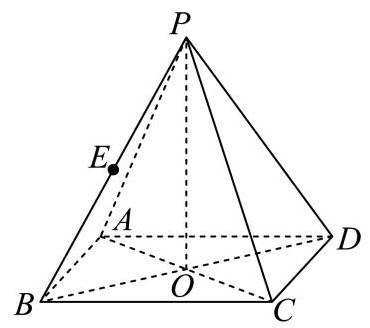
\includegraphics[max width=0.2\textwidth]{images/bo_d6dcisv7aajc739b5agg_14_257_465_370_328_0.jpg}
\end{center}
\hspace*{3em} 

(1)若 \({AP} = 5,{AD} = {3\sqrt{2}}\) ，求 \(\bigtriangleup  {POA}\) 绕 \({PO}\) 旋转一周形成的几何体的体积；

(2)若 \({AP} = {AD},E\) 为 \({PB}\) 的中点，求直线 \({BD}\) 与平面 \({AEC}\) 所成角的大小.

19. 为了解某地初中学生体育锻炼时长与学业成绩的关系, 从该地区 29000 名学生中抽取 580 人，得到日均体育锻炼时长与学业成绩的数据如下表所示:

\begin{center}
\adjustbox{max width=\textwidth}{
\begin{tabular}{|c|c|c|c|c|c|}
\hline
时间范围学业成绩 & \(\lbrack 0,{0.5})\) & \(\lbrack {0.5},1)\) & \(\lbrack 1,{1.5})\) & \(\lbrack {1.5},2)\) & \(\lbrack 2,{2.5})\) \\
\cline{1-6}
优秀 & 5 & 44 & 42 & 3 & 1 \\
\cline{1-6}
不优秀 & 134 & 147 & 137 & 40 & 27 \\
\cline{1-6}
\hline
\end{tabular}
}
\end{center}

(1)该地区 29000 名学生中体育锻炼时长不少于 1 小时人数约为多少？

(2)估计该地区初中学生日均体育锻炼的时长 (精确到 0.1)

(3)是否有 95\% 的把握认为学业成绩优秀与日均体育锻炼时长不小于 1 小时且小于 2 小时有关？

20. 已知双曲线 \(\Gamma  : {x}^{2} - \frac{{y}^{2}}{{b}^{2}} = 1,\;\left( {b > 0}\right)\) ,左右顶点分别为 \({A}_{1},{A}_{2}\) ,过点 \(M\left( {-2,0}\right)\) 的直线 \(l\) 交双曲线 \(\Gamma\) 于 \(P,Q\) 两点.

(1)若离心率 \(\mathrm{e} = 2\) 时，求 \(b\) 的值.

(2)若 \(b = \frac{2\sqrt{6}}{3}\) ， \(\bigtriangleup  M{A}_{2}P\) 为等腰三角形时，且点 \(P\) 在第一象限，求点 \(P\) 的坐标.

(3)连接 \({OQ}\) 并延长，交双曲线 \(\Gamma\) 于点 \(R\) ，若 \(\overrightarrow{{A}_{1}R} \cdot  \overrightarrow{{A}_{2}P} = 1\) ，求 \(b\) 的取值范围.

21. 对于一个函数 \(f\left( x\right)\) 和一个点 \(M\left( {a,b}\right)\) ,令 \(s\left( x\right)  = {\left( x - a\right) }^{2} + {\left( f\left( x\right)  - b\right) }^{2}\) ,若 \(P\left( {{x}_{0},f\left( {x}_{0}\right) }\right)\) 是 \(s\left( x\right)\) 取到最小值的点,则称 \(P\) 是 \(M\) 在 \(f\left( x\right)\) 的 “最近点”.

(1)对于 \(f\left( x\right)  = \frac{1}{x}\left( {x > 0}\right)\) ，求证:对于点 \(M\left( {0,0}\right)\) ，存在点 \(P\) ，使得点 \(P\) 是 \(M\) 在 \(f\left( x\right)\) 的 “最近点”;

(2)对于 \(f\left( x\right)  = {\mathrm{e}}^{x},M\left( {1,0}\right)\) ，请判断是否存在一个点 \(P\) ，它是 \(M\) 在 \(f\left( x\right)\) 的 “最近点”，且直线 \({MP}\) 与 \(y = f\left( x\right)\) 在点 \(P\) 处的切线垂直;

(3) 已知 \(y = f\left( x\right)\) 在定义域 \(R\) 上存在导函数 \({f}^{\prime }\left( x\right)\) ，且函数 \(g\left( x\right)\) 在定义域 \(R\) 上恒正，设点

\({M}_{1}\left( {t - 1,f\left( t\right)  - g\left( t\right) }\right) ,{M}_{2}\left( {t + 1,f\left( t\right)  + g\left( t\right) }\right)\) . 若对任意的 \(t \in  R\) ，存在点 \(P\) 同时是 \({M}_{1}\) ， \({M}_{2}\) 在 \(f\left( x\right)\) 的 “最近点”,试判断 \(f\left( x\right)\) 的单调性.

\section*{24春}

\section*{一、填空题}

1. 函数 \(f\left( x\right)  = {\log }_{2}x\) 的定义域是\_\_\_\_\_

2. 直线 \(x - y + 1 = 0\) 的倾斜角大小为\_\_\_\_\_.

3. 已知 \(\frac{Z}{1 + i} = \mathrm{i}\) ，则 \(\bar{z} =\) \_\_\_\_\_.

4. \({\left( x - 1\right) }^{6}\) 展开式中 \({x}^{4}\) 的系数为\_\_\_\_\_.

5. 三角形 \({ABC}\) 中， \({BC} = 2,A = \frac{\pi }{3},B = \frac{\pi }{4}\) ，则 \({AB} =\) \_\_\_\_\_.

6. 已知 \({ab} = 1,\;4{a}^{2} + 9{b}^{2}\) 的最小值为\_\_\_\_\_.

7. 数列 \(\left\{  {a}_{n}\right\}  ,{a}_{n} = n + c,{S}_{7} < 0,c\) 的取值范围为\_\_\_\_\_.

8. 三角形三边长为5，6，7，则以边长为6的两个顶点为焦点，过另外一个顶点的双曲线的离心率为\_\_\_\_\_.

9. 已知 \(f\left( x\right)  = {x}^{2},g\left( x\right)  = \left\{  \begin{array}{ll} f\left( x\right) , & x \geq  0 \\   - f\left( {-x}\right) , & x < 0 \end{array}\right.\) ，求 \(g\left( x\right)  \leq  2 - x\) 的 \(x\) 的取值范围\_\_\_\_\_.

10. 已知四棱柱 \({ABCD} - {A}_{1}{B}_{1}{C}_{1}{D}_{1}\) 底面 \({ABCD}\) 为平行四边形， \(A{A}_{1} = 3\) ， \({BD} = 4\) 且 \(\overrightarrow{A{B}_{1}} \cdot  \overrightarrow{BC} \; - \overrightarrow{A{D}_{1}} \cdot  \overrightarrow{DC} = 5\) ，则异面直线 \(A{A}_{1}\) 与 \({BD}\) 的夹角余弦值为\_\_\_\_\_.

\begin{center}
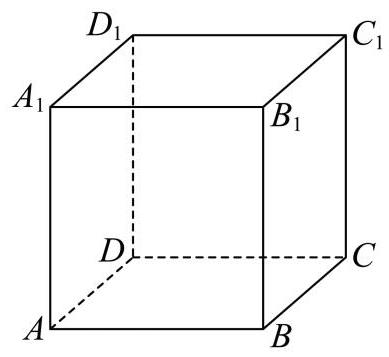
\includegraphics[max width=0.3\textwidth]{images/bo_d6dcisv7aajc739b5agg_17_259_664_389_357_0.jpg}
\end{center}
\hspace*{3em} 

11. 正方形草地 \({ABCD}\) 边长 1.2 ， \(E\) 到 \({AB}\) ， \({AD}\) 距离为 0.2， \(F\) 到 \({BC}\) ， \({CD}\) 距离为 0.4，有个圆形通道经过 \(E\) ， \(F\) ，且经过 \({AD}\) 上一点，求圆形通道的周长\_\_\_\_\_. (精确到 0.01)

\begin{center}
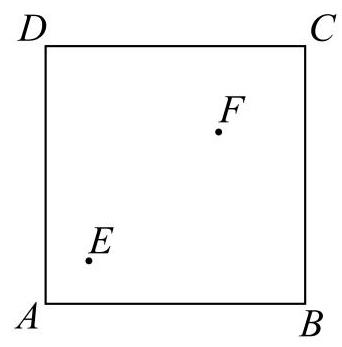
\includegraphics[max width=0.2\textwidth]{images/bo_d6dcisv7aajc739b5agg_17_253_1362_342_347_0.jpg}
\end{center}
\hspace*{3em} 

12. \({a}_{1} = 2,\;{a}_{2} = 4,\;{a}_{3} = 8,\;{a}_{4} = {16}\) ,任意 \({b}_{1},\;{b}_{2},\;{b}_{3},\;{b}_{4} \in  R\) ,满足 \(\left\{  {{a}_{i} + {a}_{j} \mid  1 \leq  i < j \leq  4}\right\}   = \; \left\{  {{b}_{i} + {b}_{j} \mid  1 \leq  \mathrm{i} < j \leq  4}\right\}\) ，求有序数列 \(\left\{  {{b}_{1},{b}_{2},{b}_{3},{b}_{4}}\right\}\) 有\_\_\_\_\_对.

二、选择题

13. \(a,b,c \in  R,b > c\) ,下列不等式恒成立的是 ( )

A. \(a + {b}^{2} > a + {c}^{2}\) B. \({a}^{2} + b > {a}^{2} + c\) C. \(a{b}^{2} > a{c}^{2}\) D. \({a}^{2}b > {a}^{2}c\)

14. 空间中有两个不同的平面 \(\alpha ,\beta\) 和两条不同的直线 \(m,n\) ，则下列说法中正确的是 ( )

A. 若 \(\alpha  \bot  \beta ,m \bot  \alpha ,n \bot  \beta\) ,则 \(m \bot  n\) B. 若 \(\alpha  \bot  \beta ,m \bot  \alpha ,m \bot  n\) ,则 \(n \bot  \beta\)

C. 若 \(\alpha //\beta ,m//\alpha ,n//\beta\) ,则 \(m//n\) D. 若 \(\alpha //\beta ,m//\alpha ,m//n\) ,则 \(n//\beta\)

15. 有四种礼盒，前三种里面分别仅装有中国结、记事本、笔袋，第四个礼盒里面三种礼品都有,现从中任选一个盒子,设事件 \(A\) : 所选盒中有中国结,事件 \(B\) : 所选盒中有记事本, 事件 \(C\) : 所选盒中有笔袋,则 ( )

A. 事件 \(A\) 与事件 \(B\) 互斥 B. 事件 \(A\) 与事件 \(B\) 相互独立

C. 事件 \(A\) 与事件 \(B \cup  C\) 互斥 D. 事件 \(A\) 与事件 \(B \cap  C\) 相互独立

16. 现定义如下: 当 \(x \in  \left( {n,n + 1}\right)\) 时 \(\left( {n \in  N}\right)\) ,若 \(f\left( {x + 1}\right)  = {f}^{\prime }\left( x\right)\) ,则称 \(f\left( x\right)\) 为延展函数. 已知当 \(x \in  \left( {0,1}\right)\) 时, \(g\left( x\right)  = {\mathrm{e}}^{x}\) 且 \(h\left( x\right)  = {x}^{10}\) ,且 \(g\left( x\right) ,h\left( x\right)\) 均为延展函数,则以下结论

( )

(1)存在 \(y = {kx} + b\left( {k,b \in  R,k,b \neq  0}\right)\) 与 \(y = g\left( x\right)\) 有无穷个交点

(2) 存在 \(y = {kx} + b\left( {k,b \in  R,k,b \neq  0}\right)\) 与 \(y = h\left( x\right)\) 有无穷个交点

A. \(\left( 1\right) \left( 2\right)\) 都成立 B. \(\left( 1\right) \left( 2\right)\) 都不成立

C. \(\left( 1\right)\) 成立 \(\left( 2\right)\) 不成立 D. \(\left( 1\right)\) 不成立 \(\left( 2\right)\) 成立.

\section*{三、解答题}

17. 已知 \(f\left( x\right)  = \sin \left( {{\omega x} + \frac{\pi }{3}}\right) ,\omega  > 0\)

(1) 设 \(\omega  = 1\) ,求解: \(y = f\left( x\right) ,x \in  \left\lbrack  {0,\pi }\right\rbrack\) 的值域;

(2) \(a > \pi \left( {a \in  R}\right) ,f\left( x\right)\) 的最小正周期为 \(\pi\) ,若在 \(x \in  \left\lbrack  {\pi ,a}\right\rbrack\) 上恰有 3 个零点,求 \(a\) 的取值范围.

18. 如图, \({PA}\text{ 、 }{PB}\text{ 、 }{PC}\) 为圆锥三条母线, \({AB} = {AC}\) .

\begin{center}
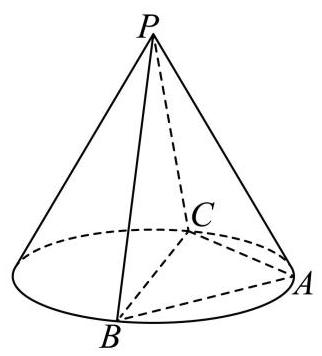
\includegraphics[max width=0.2\textwidth]{images/bo_d6dcisv7aajc739b5agg_19_259_905_322_356_0.jpg}
\end{center}
\hspace*{3em} 

(1)证明: \({PA} \bot  {BC}\) ；

(2)若圆锥侧面积为 \({\sqrt{3}\pi },{BC}\) 为底面直径， \({BC} = 2\) ，求二面角 \(B - {PA} - C\) 的大小

19. 水果分为一级果和二级果, 共 136 箱, 其中一级果 102 箱, 二级果 34 箱.

(1)随机挑选两箱水果，求恰好一级果和二级果各一箱的概率；

(2)进行分层抽样，共抽 8 箱水果，求一级果和二级果各几箱；

(3)抽取若干箱水果，其中一级果共 120 个，单果质量平均数为 303.45 克，方差为 603.46；二级果 48 个, 单果质量平均数为 240.41 克, 方差为 648.21; 求 168 个水果的方差和平均数, 并预估果园中单果的质量.

20. 在平面直角坐标系 \({xOy}\) 中,已知点 \(A\) 为椭圆 \(\Gamma  : \frac{{x}^{2}}{6} + \frac{{y}^{2}}{2} = 1\) 上一点, \({F}_{1}\text{ 、 }{F}_{2}\) 分别为椭圆的左、右焦点.

(1)若点 \(A\) 的横坐标为 2，求 \(\left| {A{F}_{1}}\right|\) 的长；

(2)设 \(\Gamma\) 的上、下顶点分别为 \({M}_{1}\) 、 \({M}_{2}\) ，记 \(\bigtriangleup  A{F}_{1}{F}_{2}\) 的面积为 \({S}_{1}\) ， \(\bigtriangleup  A{M}_{1}{M}_{2}\) 的面积为 \({S}_{2}\) ，若 \({S}_{1} \; \geq  {S}_{2}\) ,求 \(\left| {OA}\right|\) 的取值范围

(3)若点 \(A\) 在 \(x\) 轴上方，设直线 \(A{F}_{2}\) 与 \(\Gamma\) 交于点 \(B\) ，与 \(y\) 轴交于点 \(K\) ， \(K{F}_{1}\) 延长线与 \(\Gamma\) 交于点

\(C\) ,是否存在 \(x\) 轴上方的点 \(C\) ,使得 \(\overrightarrow{{F}_{1}A} + \overrightarrow{{F}_{1}B} + \overrightarrow{{F}_{1}C} = \lambda \left( {\overrightarrow{{F}_{2}A} + \overrightarrow{{F}_{2}B} + \overrightarrow{{F}_{2}C}}\right) \left( {\lambda  \in  R}\right)\) 成立? 若存在,请求出点 \(C\) 的坐标; 若不存在,请说明理由.

21. 记 \(M\left( a\right)  = \{ t \mid  t = f\left( x\right)  - f\left( a\right) ,x \geq  a\} ,\;L\left( a\right)  = \{ t \mid  t = f\left( x\right)  - f\left( a\right) ,x \leq  a\}\)

(1)若 \(f\left( x\right)  = {x}^{2} + 1\) ，求 \(M\left( 1\right)\) 和 \(L\left( 1\right)\) ；

(2)若 \(f\left( x\right)  = {x}^{3} - 3{x}^{2}\) ，求证:对于任意 \(a \in  R\) ，都有 \(M\left( a\right)  \subseteq  \lbrack  - 4, + \infty )\) ，且存在 \(a\) ，使得 -4 ∈ \(M\left( a\right)\) .

(3)已知定义在 \(R\) 上 \(f\left( x\right)\) 有最小值，求证 " \(f\left( x\right)\) 是偶函数 "的充要条件是 "对于任意正实数 \(c\) ， 均有 \(M\left( {-c}\right)  = L\left( c\right)\) ” .

\section*{23 秋考}

一、填空题(本大题共有 12 题，满分 54 分，第 1-6 题每题 4 分，第 7-12 题每题 5 分) 1. 不等式 \(\left| {x - 2}\right|  < 1\) 的解集为\_\_\_\_\_.

2. 已知向量 \(\overrightarrow{a} = \left( {-2,3}\right) ,\;\overrightarrow{b} = \left( {1,2}\right)\) ，则 \(\overrightarrow{a} \cdot  \overrightarrow{b} =\) \_\_\_\_\_.

3. 已知首项为3，公比为2的等比数列，设等比数列的前 \(n\) 项和为 \({S}_{n}\) ，则 \({S}_{6} =\) \_\_\_\_\_.

4. 已知 \(\tan \alpha  = 3\) ，则 \(\tan {2\alpha } =\) \_\_\_\_\_.

5. 已知函数 \(f\left( x\right)  = \left\{  \begin{array}{l} 1,x \leq  0, \\  {2}^{x},x > 0 \end{array}\right.\) ,则函数 \(f\left( x\right)\) 的值域为\_\_\_\_\_.

6. 已知复数 \(z = 1 - \mathrm{i}\) ( \(\mathrm{i}\) 为虚数单位),则 \(\left| {1 + {iz}}\right|  =\) \_\_\_\_\_.

7. 已知圆 \({x}^{2} + {y}^{2} - {4x} - m = 0\) 的面积为 \(\pi\) ，则 \(m =\) \_\_\_\_\_.

8. 已知 \({ABC}\) 中，角 \(A,B,C\) 所对的边 \(a = 4,b = 5,c = 6\) ，则 \(\sin A =\) \_\_\_\_\_.

9. 国内生产总值 (GDP) 是衡量一个国家或地区经济状况和发展水平的重要指标，根据统计数据显示，某市在 2020 年间经济高质量增长， \({GDP}\) 稳步增长，第一季度 \({GDP}\) 为 232 亿元， 第四季度 \({GDP}\) 为 241 亿元，四个季度的 \({GDP}\) 逐季度增长，且中位数与平均数相同，则该地一年的 \({GDP}\) 为\_\_\_\_\_亿元.

10. 已知 \({\left( 1 + {2023}x\right) }^{100} + {\left( {2023} - x\right) }^{100} = {a}_{0} + {a}_{1}x + {a}_{2}{x}^{2} +  + {a}_{99}{x}^{99} + {a}_{100}{x}^{100}\) ,若存在 \(k \in \; \{ 0,1,2,1,{100}\}\) 使得 \({a}_{k} < 0\) ，则 \(k\) 的最大值为\_\_\_\_\_.

11. 某公园欲建设一段斜坡，坡顶是一条直线，斜坡顶点距水平地面的高度为 4 米，坡面与水平面所成夹角为 \(\theta\) . 行人每沿着斜坡向上走 \(1\mathrm{m}\) 消耗的体力为 \(\left( {{1.025} - \cos \theta }\right)\) ,欲使行人走上斜坡所消耗的总体力最小，则 \(\theta  =\) \_\_\_\_\_.

12. 空间中有三个点 \(A\text{ 、 }B\text{ 、 }C\) ,且 \({AB} = {BC} = {CA} = 1\) ,在空间中任取 2 个不同的点 (不计顺序), 使得它们与 \(A\) 、 \(B\) 、 \(C\) 恰好成为一个正四棱锥的五个顶点, 则不同的取法有\_\_\_\_\_.

二、选择题 (本大题共有 4 题,满分 18 分,第 \({13} - {14}\) 题每题 4 分,第 \({15} - {16}\) 题每题 5 分) 每题有且只有一个正确答案.

13. 已知 \(P = \{ 1,2\} ,Q = \{ 2,3\}\) ,若 \(M = \{ x \mid  x \in  P,x \notin  Q\}\) ,则 \(M =\) ( )

A. \(\{ 1\}\) B. \{2\} C. \{3\} D. \(\{ 1,2,3\}\)

14. 已知某校 50 名学生的身高和体重散点图如图所示, 则下列说法正确的是 ( )

\begin{center}
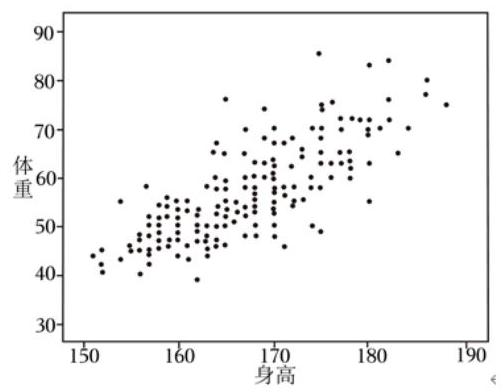
\includegraphics[max width=0.3\textwidth]{images/bo_d6dcisv7aajc739b5agg_23_258_916_503_392_0.jpg}
\end{center}
\hspace*{3em} 

A. 身高越大，体重越大 B. 身高越大，体重越小

C. 身高和体重成正相关 D. 身高和体重成负相关

15. 已知 \(a > 0\) ,记 \(y = \sin x\) 在 \(\left\lbrack  {a,{2a}}\right\rbrack\) 的最小值为 \({s}_{a}\) ,在 \(\left\lbrack  {{2a},{3a}}\right\rbrack\) 的最小值为 \({t}_{a}\) ,则下列情况不可能的是 ( )

A. \({s}_{a} > 0,{t}_{a} > 0\) B. \({s}_{a} < 0,{t}_{a} < 0\) C. \({s}_{a} > 0,{t}_{a} < 0\) D. \({s}_{a} < 0,{t}_{a} > 0\)

16. 已知 \(P,Q\) 是曲线 \(\Gamma\) 上两点,若存在 \(M\) 点,使得曲线 \(\Gamma\) 上任意一点 \(P\) 都存在 \(Q\) 使得 \(\left| {MP}\right|\) .

\(\left| {MQ}\right|  = 1\) ,则称曲线 \(\Gamma\) 是 “自相关曲线”. 现有如下两个命题:  \circled{1} 任意椭圆都是 “自相关曲线”;  \circled{2} 存在双曲线是 “自相关曲线”，则 ( )

A.  \circled{1} 成立， \circled{2} 成立 B.  \circled{1} 成立， \circled{2} 不成立

C.  \circled{1} 不成立， \circled{2} 成立 D.  \circled{1} 不成立， \circled{2} 不成立

三、解答题 (本大题共有 5 题, 满分 78 分) 解答下列各题必须在答题纸的相应位置写出必要的步骤.

17. 已知直四棱柱 \({ABCD} - {A}_{1}{B}_{1}{C}_{1}{D}_{1},{AB} \bot  {AD},{AB}//{CD},{AB} = 2,{AD} = 3,{CD} = 4\) .

\begin{center}
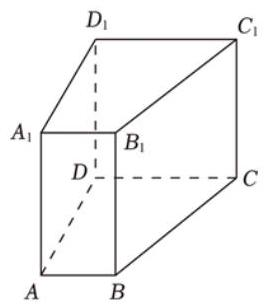
\includegraphics[max width=0.2\textwidth]{images/bo_d6dcisv7aajc739b5agg_24_257_794_269_306_0.jpg}
\end{center}
\hspace*{3em} 

(1)证明:直线 \({A}_{1}B//\) 平面 \({DC}{C}_{1}{D}_{1}\) ;

(2)若该四棱柱的体积为 36，求二面角 \({A}_{1} - {BD} - A\) 的大小.

18. 已知 \(a,c \in  R\) ,函数 \(f\left( x\right)  = \frac{{x}^{2} + \left( {{3a} + 1}\right) x + c}{x + a}\) .

(1)若 \(a = 0\) ，求函数的定义域，并判断是否存在 \(c\) 使得 \(f\left( x\right)\) 是奇函数，说明理由；

(2)若函数过点 \(\left( {1,3}\right)\) ，且函数 \(f\left( x\right)\) 与 \(x\) 轴负半轴有两个不同交点，求此时 \(c\) 的值和 \(a\) 的取值范围.

19. 2023 年 6 月 7 日, 21 世纪汽车博览会在上海举行, 已知某汽车模型公司共有 25 个汽车模型, 其外观和内饰的颜色分布如下表所示:

\begin{center}
\adjustbox{max width=\textwidth}{
\begin{tabular}{|c|c|c|}
\hline
\phantom{X} & 红色外观 & 蓝色外观 \\
\cline{1-3}
米色内饰 & 8 & 12 \\
\cline{1-3}
棕色内饰 & 2 & 3 \\
\cline{1-3}
\hline
\end{tabular}
}
\end{center}

(1)若小明从这些模型中随机拿一个模型，记事件 \(A\) 为小明取到红色外观的模型，事件 \(B\) 为小明取到棕色内饰的模型,求 \(P\left( B\right)\) 和 \(P\left( {B \mid  A}\right)\) ,并判断事件 \(A\) 和事件 \(B\) 是否独立;

(2)该公司举行了一个抽奖活动，规定在一次抽奖中，每人可以一次性从这些模型中拿两个汽车模型, 给出以下假设:

20. 已知抛物线 \(\Gamma  : {y}^{2} = {4x}\) ,在 \(\Gamma\) 上有一点 \(A\) 位于第一象限,设 \(A\) 的纵坐标为 \(a\left( {a0}\right)\) .

(1)若 \(A\) 到抛物线 \(\Gamma\) 准线的距离为3，求 \(a\) 的值；

(2) 当 \(a = 4\) 时,若 \(x\) 轴上存在一点 \(B\) ,使 \({AB}\) 的中点在抛物线 \(\Gamma\) 上,求 \(O\) 到直线 \({AB}\) 的距离;

(3) 直线 \(l : x =  - 3,P\) 是第一象限 \(\Gamma\) 上异于 \(A\) 的一点, \(P\) 在直线 \(l\) 上的投影为点 \(H\) ,直线 \({AP}\) 与直线 \(l\) 的交点为 \(Q\) . 若在 \(P\) 的位置变化过程中, \(\left| {HQ}\right|  > 4\) 恒成立,求 \(a\) 的取值范围.

21. 已知 \(f\left( x\right)  = \ln x\) ,在该函数图象 \(\Gamma\) 上取一点 \({a}_{1}\) ,过点 \(\left( {{a}_{1},f\left( {a}_{1}\right) }\right)\) ,作函数 \(f\left( x\right)\) 的切线,该切线与 \(y\) 轴的交点记作 \(\left( {0,{a}_{2}}\right)\) ,若 \({a}_{2} > 0\) ,则过点 \(\left( {{a}_{2},f\left( {a}_{2}\right) }\right)\) ,作函数 \(f\left( x\right)\) 的切线,该切线与 \(y\) 轴的交点记作 \(\left( {0,{a}_{3}}\right)\) ,以此类推,直至 \({a}_{n} \leq  0\left( {n \in  {N}^{ * }}\right)\) 停止,由这些项构成数列 \(\left\{  {a}_{n}\right\}\) .

(1)若正整数 \(m \geq  2\) ，证明: \({a}_{m} = \ln {a}_{m - 1} - 1\) ；

(2)若正整数 \(m \geq  2\) ，试比较 \({a}_{m}\) 与 \({a}_{m - 1} - 2\) 的大小关系；

(3)若正整数 \(k \geq  3\) ，是否存在 \(k\) 使得 \({a}_{1}\text{ 、 }{a}_{2}\text{ 、 }{a}_{3}\text{ 、 }\cdots \text{ 、 }{a}_{k}\) 依次成等差数列? 若存在，求出 \(k\) 的所有取值; 若不存在, 请说明理由.

\section*{23 春考}

一、填空题(本大题共有 12 题，满分 54 分，第 1-6 题每题满分 54 分，第 7-12 题每题满分 54 分) 考生应在答题纸的相应位置直接填写结果.

1. 已知集合 \(A = \{ 1,2\} ,B = \{ 1,a\}\) ，且 \(A = B\) ，则 \(a =\) \_\_\_\_\_.

2. 已知向量 \(\overrightarrow{a} = \left( {3,4}\right)\) ， \(\overrightarrow{b} = \left( {1,2}\right)\) ，则 \(\overrightarrow{a} - 2\overrightarrow{b} =\) \_\_\_\_\_.

3. 不等式 \(\left| {x - 1}\right|  \leq  2\) 的解集为:\_\_\_\_\_. (结果用集合或区间表示)

4. 已知圆 \(C\) 的一般方程为 \({x}^{2} + {2x} + {y}^{2} = 0\) ，则圆 \(C\) 的半径为\_\_\_\_\_.

5. 已知事件 \(A\) 的对立事件为 \(\bar{A}\) ，若 \(P\left( A\right)  = {0.5}\) ，则 \(P\left( \bar{A}\right)  =\) \_\_\_\_\_.

6. 已知正实数 \(a\) 、 \(b\) 满足 \(a + {4b} = 1\) ，则 \({ab}\) 的最大值为\_\_\_\_\_.

7. 某校抽取 100 名学生测身高, 其中身高最大值为 186cm, 最小值为 154cm, 根据身高数据绘制频率组距分布直方图，组距为 5，且第一组下限为 153.5，则组数为\_\_\_\_\_.

8. 设 \({\left( 1 - 2x\right) }^{4} = {a}_{0} + {a}_{1}x + {a}_{2}{x}^{2} + {a}_{3}{x}^{3} + {a}_{4}{x}^{4}\) ,则 \({a}_{0} + {a}_{4} =\) \_\_\_\_\_.

9. 已知函数 \(f\left( x\right)  = {2}^{-x} + 1\) ，且 \(g\left( x\right)  = \left\{  \begin{array}{l} {\log }_{2}\left( {x + 1}\right) ,x \geq  0 \\  f\left( {-x}\right) ,x < 0 \end{array}\right.\) ，则方程 \(g\left( x\right)  = 2\) 的解为\_\_\_\_\_.

10. 为了学习宣传党的二十大精神，某校学生理论宣讲团赴社区宣讲，已知有 4 名男生，6 名女生，从 10 人中任选 3 人，则恰有 1 名男生 2 名女生的概率为\_\_\_\_\_.

11. 已知 \({z}_{1},{z}_{2} \in  C\) 且 \({z}_{1} = \mathrm{i}\overline{{z}_{2}}\) ( \(\mathrm{i}\) 为虚数单位),满足 \(\left| {{z}_{1} - 1}\right|  = 1\) ,则 \(\left| {{z}_{1} - {z}_{2}}\right|\) 的取值范围为\_\_\_\_\_.

12. 已知 \(\overrightarrow{OA}\) 、 \(\overrightarrow{OB}\) 、 \(\overrightarrow{OC}\) 为空间中三组单位向量,且 \(\overrightarrow{OA} \bot  \overrightarrow{OB}\) 、 \(\overrightarrow{OA} \bot  \overrightarrow{OC}\) , \(\overrightarrow{OB}\) 与 \(\overrightarrow{OC}\) 夹角

为 \({60} \circ\) ,点 \(P\) 为空间任意一点,且 \(\left| \overrightarrow{OP}\right|  = 1\) ,满足 \(\left| {\overrightarrow{OP} \cdot  \overrightarrow{OC}}\right|  \leq  \left| {\overrightarrow{OP} \cdot  \overrightarrow{OB}}\right|  \leq  \left| {\overrightarrow{OP} \cdot  \overrightarrow{OA}}\right|\) ,则 \(\left| {\overrightarrow{OP} \cdot  \overrightarrow{OC}}\right|\) 最大值为\_\_\_\_\_.

二、选择题 (本大题共有 4 题, 满分 18 分, 第 13-14 题每题满分 18 分, 第 15-16 题每题满分 18 分) 每题有且只有一个正确选项，考生应在答题纸相应的位置，将代表正确选项的小方格涂黑.

13. 下列函数是偶函数的 ( )

A. \(y = \sin x\) B. \(y = \cos x\) C. \(y = {x}^{3}\) D. \(y = {2}^{x}\)

14. 如图为 2017-2021 年上海市货物进出口总额的条形统计图, 则下列对于进出口贸易额描述错误的是( )

\begin{center}
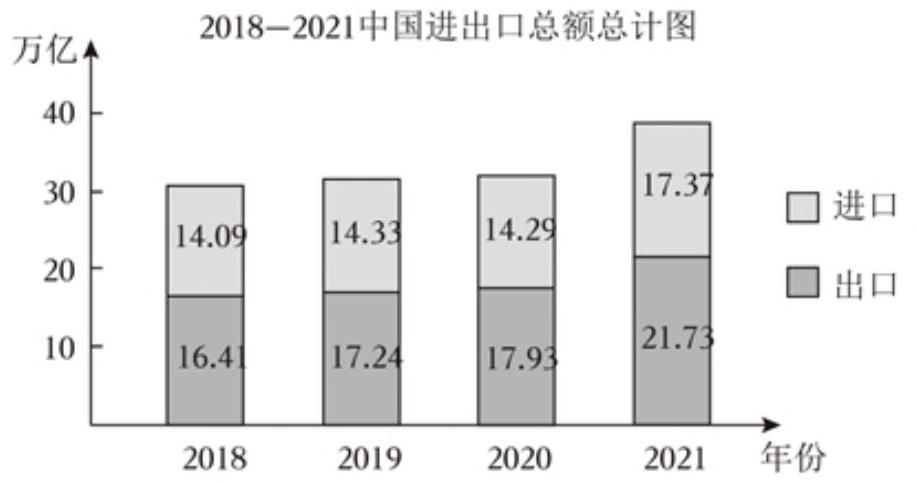
\includegraphics[max width=0.7\textwidth]{images/bo_d6dcisv7aajc739b5agg_29_270_1207_917_483_0.jpg}
\end{center}
\hspace*{3em} 

A. 从 2018 年开始, 2021 年的进出口总额增长率最大

B. 从 2018 年开始, 进出口总额逐年增大

C. 从 2018 年开始, 进口总额逐年增大

D. 从 2018 年开始, 2020 年的进出口总额增长率最小

15. 如图所示,在正方体 \({ABCD} - {A}_{1}{B}_{1}{C}_{1}{D}_{1}\) 中,点 \(P\) 为边 \({A}_{1}{C}_{1}\) 上的动点,则下列直线中,始终与直线 \({BP}\) 异面的是 ( )

\begin{center}
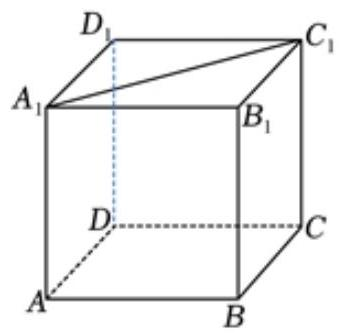
\includegraphics[max width=0.2\textwidth]{images/bo_d6dcisv7aajc739b5agg_30_278_320_341_335_0.jpg}
\end{center}
\hspace*{3em} 

A. \(D{D}_{1}\) B. \({AC}\) C. \(A{D}_{1}\) D. \({B}_{1}C\)

16. 已知无穷数列 \(\left\{  {a}_{n}\right\}\) 的各项均为实数， \({S}_{n}\) 为其前 \(n\) 项和，若对任意正整数 \(k > {2022}\) 都有 \(\left| {S}_{k}\right| \; > \left| {S}_{k + 1}\right|\) ,则下列各项中可能成立的是 ( )

A. \({a}_{1},{a}_{3},{a}_{5},\cdots ,{a}_{{2n} - 1},\cdots\) 为等差数到， \({a}_{2},{a}_{4},{a}_{6},\cdots ,{a}_{2n},\cdots\) 为等比数列

B. \({a}_{1}\) ， \({a}_{3}\) ， \({a}_{5}\) ， \(\cdots\) ， \({a}_{{2n} - 1}\) ， \(\cdots\) 为等比数列， \({a}_{2}\) ， \({a}_{4}\) ， \({a}_{6}\) ， \(\cdots\) ， \({a}_{2n}\) ， \(\cdots\) 为等差数列

C. \({a}_{1}\) ， \({a}_{2}\) ， \({a}_{3}\) ， \(\cdots\) ， \({a}_{2022}\) 为等差数列， \({a}_{2022}\) ， \({a}_{2023}\) ， \(\cdots\) ， \({a}_{n}\) ， \(\cdots\) 为等比数列

D. \({a}_{1},{a}_{2},{a}_{3},\cdots ,{a}_{2022}\) 为等比数列, \({a}_{2022},{a}_{2023},\cdots ,{a}_{n},\cdots\) 为等差数列

三、解答题 (本大题共有 5 题, 满分 78 分) 解答下列各题必须在答题纸的相应位置写出必要的步骤。

17. 已知三棱锥 \(P - {ABC}\) 中， \({PA}\bot\) 平面 \({ABC}\) ， \({AB}\bot {AC}\) ， \({PA} = {AB} = 3\) ， \({AC} = 4\) ， \(M\) 为 \({BC}\) 中点,过点 \(M\) 分别作平行于平面 \({PAB}\) 的直线交 \({AC}\text{ 、 }{PC}\) 于点 \(E,F\) .

\begin{center}
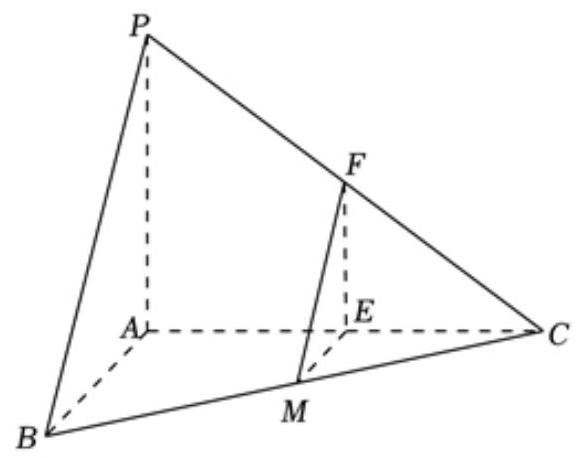
\includegraphics[max width=0.4\textwidth]{images/bo_d6dcisv7aajc739b5agg_31_258_463_580_458_0.jpg}
\end{center}
\hspace*{3em} 

(1)求直线 \({PM}\) 与平面 \({ABC}\) 所成角的大小；

(2)求直线 \({ME}\) 到平面 \({PAB}\) 的距离.

18. 在 \({ABC}\) 中,角 \(A\text{ 、 }B\text{ 、 }C\) 所对应的边分别为 \(a\text{ 、 }b\text{ 、 }c\) ,其中 \(b = 2\) .

(1) 若 \(A + C = {120}^{ \circ  },a = {2c}\) ,求边长 \(c\) ;

(2)若 \(A - C = {15}^{ \circ  },\;a = \sqrt{2}c\sin A\) ，求 \({\Delta ABC}\) 的面积.

19. 为了节能环保、节约材料,定义建筑物的“体形系数” \(S = \frac{{F}_{0}}{{V}_{0}}\) ,其中 \({F}_{0}\) 为建筑物暴露在空气中的面积 (单位:平方米)， \({V}_{0}\) 为建筑物的体积 (单位:立方米).

(1)若有一个圆柱体建筑的底面半径为 \(R\) ，高度为 \(H\) ，暴露在空气中的部分为上底面和侧面， 试求该建筑体的 “体形系数” \(S\) ; (结果用含 \(R\) 、 \(H\) 的代数式表示)

(2)定义建筑物的 “形状因子” 为 \(f = \frac{{L}^{2}}{A}\) ，其中 \(A\) 为建筑物底面面积， \(L\) 为建筑物底面周长， 又定义 \(T\) 为总建筑面积,即为每层建筑面积之和 (每层建筑面积为每一层的底面面积). 设 \(n\) 为某宿舍楼的层数,层高为 3 米,则可以推导出该宿舍楼的 “体形系数” 为 \(S = \sqrt{\frac{f \cdot  n}{T}} + \frac{1}{3n}\) . 当 \(f = {18},T = {10000}\) 时,试求当该宿舍楼的层数 \(n\) 为多少时,“体形系数” \(S\) 最小.

20. 已知椭圆 \(\Gamma  : \frac{{x}^{2}}{{m}^{2}} + \frac{{y}^{2}}{3} = 1\left( {{m0}\text{ 且 }m \neq  \sqrt{3}}\right)\) .

(1)若 \(m = 2\) ，求椭圆 \(\Gamma\) 的离心率；

(2)设 \({A}_{1}\) 、 \({A}_{2}\) 为椭圆 \(\Gamma\) 的左右顶点，椭圆 \(\Gamma\) 上一点 \(E\) 的纵坐标为1，且 \(\overrightarrow{E{A}_{1}} \cdot  \overrightarrow{E{A}_{2}} =  - 2\) ，求实数 \(m\) 的值;

(3)过椭圆 \(\Gamma\) 上一点 \(P\) 作斜率为 \(\sqrt{3}\) 的直线 \(l\) ，若直线 \(l\) 与双曲线 \(\frac{{y}^{2}}{5{m}^{2}} - \frac{{x}^{2}}{5} = 1\) 有且仅有一个公共点,求实数 \(m\) 的取值范围.

21. 已知函数 \(f\left( x\right)  = a{x}^{3} - \left( {a + 1}\right) {x}^{2} + x,g\left( x\right)  = {kx} + m\) (其中 \(a \geq  0,k,m \in  R\) ),若任意 \(x \in \; \left\lbrack  {0,1}\right\rbrack\) 均有 \(f\left( x\right)  \leq  g\left( x\right)\) ,则称函数 \(y = g\left( x\right)\) 是函数 \(y = f\left( x\right)\) 的 “控制函数”,且对所有满足条件的函数 \(y = g\left( x\right)\) 在 \(x\) 处取得的最小值记为 \(\bar{f}\left( x\right)\) .

(1) 若 \(a = 2,g\left( x\right)  = x\) ,试判断函数 \(y = g\left( x\right)\) 是否为函数 \(y = f\left( x\right)\) 的“控制函数”,并说明理由;

( 2 )若 \(a = 0\) ，曲线 \(y = f\left( x\right)\) 在 \(x = \frac{1}{4}\) 处的切线为直线 \(y = h\left( x\right)\) ，证明:函数 \(y = h\left( x\right)\) 为函数 \(y \; = f\left( x\right)\) 的 “控制函数”,并求 \(\bar{f}\left( \frac{1}{4}\right)\) 的值;

(3)若曲线 \(y = f\left( x\right)\) 在 \(x = {x}_{0},{x}_{0} \in  \left( {0,1}\right)\) 处的切线过点 \(\left( {1,0}\right)\) ，且 \(c \in  \left\lbrack  {{x}_{0},1}\right\rbrack\) ，证明:当且仅当 \(c = {x}_{0}\) 或 \(c = 1\) 时, \(\bar{f}\left( c\right)  = f\left( c\right)\) .

\section*{课改前}

\section*{2011 秋考}

\section*{填空}

1. 函数 \(f\left( x\right)  = \frac{1}{x - 2}\) 的反函数为 \({f}^{-1}\left( x\right)  =\) \_\_\_\_\_.

2. 若全集 \(U = R\) ，集合 \(A = \{ x \mid  x \geq  1\}  \cup  \{ x \mid  x \leq  0\}\) ，则 \({\complement }_{U}A =\) \_\_\_\_\_.

3. 设 \(m\) 是常数，若点 \(F\left( {0,5}\right)\) 是双曲线 \(\frac{{y}^{2}}{m} - \frac{{x}^{2}}{9} = 1\) 的一个焦点，则 \(m =\) \_\_\_\_\_.

4. 不等式 \(\frac{x + 1}{x} < 3\) 的解为\_\_\_\_\_.

5. 在极坐标系中,直线 \(\rho \left( {2\cos \theta  + \sin \theta }\right)  = 2\) 与直线 \(\rho \cos \theta  = 1\) 的夹角大小为\_\_\_\_\_. (结果用反三角函数值表示)

6. 在相距 2 千米的 \(A\) 、 \(B\) 两点处测量目标点 \(C\) ，若 \(\angle {CAB} = {75}^{ \circ  }\) ， \(\angle {CBA} = {60}^{ \circ  }\) ，则 \(A\) 、 \(C\) 两点之间的距离为\_\_\_\_\_千米.

7. 若圆锥的侧面积为 \({2\pi }\) ，底面面积为 \(\pi\) ，则该圆锥的体积为\_\_\_\_\_.

8. 函数 \(y = \sin \left( {\frac{\pi }{2} + x}\right) \cos \left( {\frac{\pi }{6} - x}\right)\) 的最大值为\_\_\_\_\_.

9. 马老师从课本上抄录一个随机变量 \(\xi\) 的概率分布列如下表:

\begin{center}
\adjustbox{max width=\textwidth}{
\begin{tabular}{|c|c|c|c|}
\hline
\(x\) & 1 & 2 & 3 \\
\cline{1-4}
\(P\left( {\xi  = x}\right)\) & ? & ! & ? \\
\cline{1-4}
\hline
\end{tabular}
}
\end{center}

请小牛同学计算 \(\xi\) 的数学期望. 尽管 “ ! ” 处完全无法看清,且两个 “? ” 处字迹模糊,但能肯定这两个 “？” 处的数值相同. 据此，小牛给出了正确答案 \({E\xi } =\) \_\_\_\_\_.

10. 行列式 \(\left| \begin{array}{ll} a & b \\  c & d \end{array}\right| \left( {a,b,c,d \in  \{  - 1,1,2\} }\right)\) 所有可能的值中,最大的是\_\_\_\_\_.

11. 在正三角形 \({ABC}\) 中， \(D\) 是 \({BC}\) 上的点. 若 \({AB} = 3,{BD} = 1\) ，则 \(\overrightarrow{AB} \cdot  \overrightarrow{AD} =\) \_\_\_\_\_.

12. 随机抽取的 9 位同学中, 至少有 2 位同学在同一月份出生的概率为\_\_\_\_\_ (默认每个月的天数相同, 结果精确到 0.001 ).

13. 已知点 \(O\left( {0,0}\right) \text{ 、 }{Q}_{0}\left( {0,1}\right)\) 和点 \({R}_{0}\left( {3,1}\right)\) ,记 \({Q}_{0}{R}_{0}\) 的中点为 \({P}_{1}\) ,取 \({Q}_{0}{P}_{1}\) 和 \({P}_{1}{R}_{0}\) 中的一条, 记其端点为 \({Q}_{1}\text{ 、 }{R}_{1}\) 使之满足 \(\left( {\left| {O{Q}_{1}}\right|  - 2}\right) \left( {\left| {O{R}_{1}}\right|  - 2}\right)  < 0\) ,记 \({Q}_{1}{R}_{1}\) 的中点为 \({P}_{2}\) ,取 \({Q}_{1}{P}_{2}\) 和 \({P}_{2}{R}_{1}\) 中的一条,记其端点为 \({Q}_{2}\text{ 、 }{R}_{2}\) ,使之满足 \(\left( {\left| {O{Q}_{2}}\right|  - 2}\right) \left( {\left| {O{R}_{2}}\right|  - 2}\right)  < 0\) . 依次下去,得到 \({P}_{1},{P}_{2},\cdots ,{P}_{n},\cdots\) ，则 \(\mathop{\lim }\limits_{{n\infty }}\left| {{Q}_{0}{P}_{n}}\right|  =\) \_\_\_\_\_.

14. 设 \(g\left( x\right)\) 是定义在 \(R\) 上,以 1 为周期的函数,若函数 \(f\left( x\right)  = x + g\left( x\right)\) 在区间 \(\left\lbrack  {3,4}\right\rbrack\) 上的值域为 \(\left\lbrack  {-2,5}\right\rbrack\) ,则 \(f\left( x\right)\) 在区间 \(\left\lbrack  {-{10},{10}}\right\rbrack\) 上的值域为\_\_\_\_\_.

15. 若 \(a,b \in  R\) ,且 \({ab} > 0\) ,则下列不等式中,恒成立的是 ().

A. \({a}^{2} + {b}^{2} > {2ab}\) B. \(a + b \geq  2\sqrt{ab}\) C. \(\frac{1}{a} + \frac{1}{b} > \frac{2}{\sqrt{ab}}\) D. \(\frac{b}{a} + \frac{a}{b} \geq  2\)

16. 下列函数中,既是偶函数,又是在区间 \(\left( {0, + \infty }\right)\) 上单调递减的函数是 ( ).

A. \(y = \ln \frac{1}{\left| x\right| }\) B. \(y = {x}^{3}\) C. \(y = {2}^{\left| x\right| }\) D. \(y = \cos x\)

17. 设 \({A}_{1},{A}_{2},{A}_{3},{A}_{4},{A}_{5}\) 是空间中给定的 5 个不同点,则使 \(\overrightarrow{M{A}_{1}} + \overrightarrow{M{A}_{2}} + \overrightarrow{M{A}_{3}} + \overrightarrow{M{A}_{4}} + \; \overrightarrow{M{A}_{5}} = \overrightarrow{0}\) 成立的点 \(M\) 的个数为 ( ).

A. 0 B. 1 C. 5 D. 10

18. 设 \(\left\{  {a}_{n}\right\}\) 是各项为正数的无穷数列, \({A}_{i}\) 是边长为 \({a}_{i},{a}_{i + 1}\) 的矩形的面积 \(\left( {\mathrm{i} = 1,2,\cdots }\right)\) ,则 \(\left\{  {A}_{n}\right\}\) 为等比数列的充要条件是 ( )

A. \(\left\{  {a}_{n}\right\}\) 是等比数列

B. \({a}_{1},{a}_{3},\cdots ,{a}_{{2n} - 1},\cdots\) 或 \({a}_{2},{a}_{4},\cdots ,{a}_{2n},\cdots\) 是等比数列

C. \({a}_{1}\) ， \({a}_{3}\) ， \(\cdots\) ， \({a}_{{2n} - 1}\) ， \(\cdots\) 和 \({a}_{2}\) ， \({a}_{4}\) ， \(\cdots\) ， \({a}_{2n}\) ， \(\cdots\) 均是等比数列

D. \({a}_{1},{a}_{3},\cdots ,{a}_{{2n} - 1},\cdots\) 和 \({a}_{2},{a}_{4},\cdots ,{a}_{2n},\cdots\) 均是等比数列,且公比相同

19. 已知复数 \({z}_{1}\) 满足 \(\left( {{z}_{1} - 2}\right) \left( {1 + \mathrm{i}}\right)  = 1 - \mathrm{i}\) ( \(\mathrm{i}\) 为虚数单位),复数 \({z}_{2}\) 的虚部为 2,且 \({z}_{1} \cdot  {z}_{2}\) 是实数, 求 \({z}_{2}\) .

20. 已知函数 \(f\left( x\right)  = a \cdot  {2}^{x} + b \cdot  {3}^{x}\) ,其中常数 \(a,b\) 满足 \(a \cdot  b \neq  0\)

(1) 若 \(a \cdot  b > 0\) ,判断函数 \(f\left( x\right)\) 的单调性;

(2)若 \(a \cdot  b < 0\) ，求 \(f\left( {x + 1}\right)  > f\left( x\right)\) 时的 \(x\) 的取值范围.

21. 已知 \({ABCD} - {A}_{1}{B}_{1}{C}_{1}{D}_{1}\) 是底面边长为 1 的正四棱柱， \({O}_{1}\) 为 \({A}_{1}{C}_{1}\) 与 \({B}_{1}{D}_{1}\) 的交点.

\begin{center}
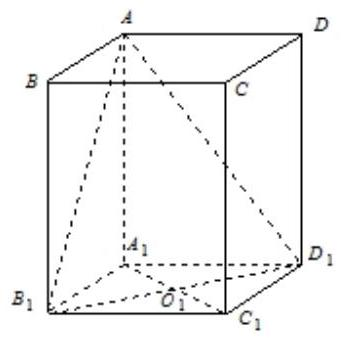
\includegraphics[max width=0.2\textwidth]{images/bo_d6dcisv7aajc739b5agg_37_259_1000_342_338_0.jpg}
\end{center}
\hspace*{3em} 

(1) 设 \(A{B}_{1}\) 与底面 \({A}_{1}{B}_{1}{C}_{1}{D}_{1}\) 所成角的大小为 \(\alpha\) ,二面角 \(A - {B}_{1}{D}_{1} - {A}_{1}\) 的大小为 \(\beta\) . 求证: \(\tan \beta  = \sqrt{2}\tan \alpha\)

(2)若点 \(C\) 到平面 \(A{B}_{1}{D}_{1}\) 的距离为 \(\frac{4}{3}\) ，求正四棱柱 \({ABCD} - {A}_{1}{B}_{1}{C}_{1}{D}_{1}\) 的高.

22. 已知数列 \(\left\{  {a}_{n}\right\}\) 和 \(\left\{  {b}_{n}\right\}\) 的通项公式分别为 \({a}_{n} = {3n} + 6,{b}_{n} = {2n} + 7\left( {n \in  {N}^{ * }}\right)\) . 将集合 \(\left\{  {x \mid  x = {a}_{n},n \in  {N}^{ * }}\right\}   \cup  \left\{  {x \mid  x = {b}_{n},n \in  {N}^{ * }}\right\}\) 中的元素从小到大依次排列,构成数列 \({c}_{1},{c}_{2},{c}_{3}\) , \(\cdots ,\;{c}_{n},\;\cdots .\)

(1)写出 \({c}_{1}\) ， \({c}_{2}\) ， \({c}_{3}\) ， \({c}_{4}\) ；

(2)求证:在数列 \(\left\{  {c}_{n}\right\}\) 中，但不在数列 \(\left\{  {b}_{n}\right\}\) 中的项恰为 \({a}_{2}\) ， \({a}_{4}\) ， \(\cdots\) ， \({a}_{2n}\) ， \(\cdots\) ；

(3)求数列 \(\left\{  {c}_{n}\right\}\) 的通项公式.

23. 已知平面上的线段 \(l\) 及点 \(P\) ,在 \(l\) 上任取一点 \(Q\) ,线段 \({PQ}\) 长度的最小值称为点 \(P\) 到线段 \(l\) 的距离,记作 \(d\left( {P,l}\right)\)

(1) 求点 \(P\left( {1,1}\right)\) 到线段 \(l : x - y - 3 = 0\left( {3 \leq  x \leq  5}\right)\) 的距离 \(d\left( {P,l}\right)\) ;

(2)设 \(l\) 是长为 2 的线段，求点的集合 \(D = \left\{  {P \mid  d\left( {P,l}\right)  \leq  1}\right\}\) 所表示的图形面积；

(3) 写出到两条线段 \({l}_{1},{l}_{2}\) 距离相等的点的集合 \(\Omega  = \left\{  {P \mid  d\left( {P,{l}_{1}}\right)  = d\left( {P,{l}_{2}}\right) }\right\}\) ,其中 \({l}_{1} = {AB},{l}_{2} = \; {CD},A,B,C,D\) 是下列三组点中的一组.

\section*{2012 秋考}

选择

1. 若 \(1 + \sqrt{2}\mathrm{i}\) 是关于 \(x\) 的实系数方程 \({x}^{2} + {bx} + c = 0\) 的一个复数根,则 ().

A. \(b = 2,c = 3\) B. \(b =  - 2,c = 3\) C. \(b =  - 2,c =  - 1\) D. \(b = 2,c =  - 1\)

2. 在 \({ABC}\) 中,若 \({\sin }^{2}A + {\sin }^{2}B < {\sin }^{2}C\) ,则 \({ABC}\) 的形状是 ().

A. 锐角三角形 B. 直角三角形 C. 钝角三角形 D. 不能确定

3. 设 \({10} \leq  {x}_{1} < {x}_{2} < {x}_{3} < {x}_{4} \leq  {10}^{4},{x}_{5} = {10}^{5}\) . 随机变量 \({\xi }_{1}\) 取值 \({x}_{1}\text{ 、 }{x}_{2}\text{ 、 }{x}_{3}\text{ 、 }{x}_{4}\text{ 、 }{x}_{5}\) 的概率均为 0.2,随机变量 \({\xi }_{2}\) 取值 \(\frac{{x}_{1} + {x}_{2}}{2}\text{ 、 }\frac{{x}_{2} + {x}_{3}}{2}\text{ 、 }\frac{{x}_{3} + {x}_{4}}{2}\text{ 、 }\frac{{x}_{4} + {x}_{5}}{2}\text{ 、 }\frac{{x}_{5} + {x}_{1}}{2}\) 的概率也为 0.2 . 若记 \(D{\widehat{\xi }}_{1}\text{ 、 }D{\widehat{\xi }}_{2}\) 分别为 \({\widehat{\xi }}_{1}\text{ 、 }{\widehat{\xi }}_{2}\) 的方差,则(   )

A. \(D{\overline{\xi }}_{1} > D{\overline{\xi }}_{2}\) B. \(D{\xi }_{1} = D{\xi }_{2}\)

C. \(D{\xi }_{1} < D{\xi }_{2}\) D. \(D{\xi }_{1}\) 与 \(D{\xi }_{2}\) 的大小关系与 \({x}_{1}\text{ 、 }{x}_{2}\text{ 、 }{x}_{3}\text{ 、 }{x}_{4}\) 的取值有关

4. 设 \({a}_{n} = \frac{1}{n}\sin \frac{n\pi }{25},{S}_{n} = {a}_{1} + {a}_{2} + \cdots  + {a}_{n}\) . 在 \({S}_{1},{S}_{2},\cdots ,{S}_{100}\) 中,正数的个数是 ().

A. 25 B. 50 C. 75 D. 100

5. 计算: \(\frac{3 - i}{1 + i} =\) \_\_\_\_\_ (i 为虚数单位).

6. 若集合 \(A = \{ x \mid  {2x} + {10}\} ,B = \{ x\left| \right| x - 1 \mid   < 2\}\) ，则 \(A \cap  B =\) \_\_\_\_\_.

7. 函数 \(f\left( x\right)  = \left| \begin{matrix} 2 & \cos x \\  \sin x &  - 1 \end{matrix}\right|\) 的值域是\_\_\_\_\_.

8. 若 \(\overrightarrow{n} = \left( {-2,1}\right)\) 是直线 \(l\) 的一个法向量，则 \(l\) 的倾斜角的大小为\_\_\_\_\_ (结果用反三角函数值表示).

9. 在 \({\left( x - \frac{2}{x}\right) }^{6}\) 的二项展开式中，常数项等于\_\_\_\_\_.

10. 有一列正方体，棱长组成以 1 为首项， \(\frac{1}{2}\) 为公比的等比数列，体积分别记为 \({V}_{1}\) ， \({V}_{2}\) ， \(\cdots\) ， \({V}_{n},\cdots\) ,则 \(\mathop{\lim }\limits_{{n\infty }}\left( {{V}_{1} + {V}_{2} + \cdots  + {V}_{n}}\right)  =\) \_\_\_\_\_.

11. 已知函数 \(f\left( x\right)  = {\mathrm{e}}^{\left| x - a\right| }\left( {a\text{ 为常数 }}\right)\) . 若 \(f\left( x\right)\) 在区间 \(\lbrack 1, + \infty )\) 上是增函数,则 \(a\) 的取值范围是\_\_\_\_\_.

12. 若一个圆锥的侧面展开图是面积为 \({2\pi }\) 的半圆面,则该圆锥的体积为\_\_\_\_\_.

13. 已知 \(y = f\left( x\right)  + {x}^{2}\) 是奇函数,且 \(f\left( 1\right)  = 1\) . 若 \(g\left( x\right)  = f\left( x\right)  + 2\) ,则 \(g\left( {-1}\right)  =\) \_\_\_\_\_.

14. 如图,在极坐标系中,过点 \(M\left( {2,0}\right)\) 的直线 \(l\) 与极轴的夹角 \(\alpha  = \frac{\pi }{6}\) . 若将 \(l\) 的极坐标方程写成 \(\rho  = f\left( \theta \right)\) 的形式，则 \(f\left( \theta \right)  =\) \_\_\_\_\_.

\begin{center}
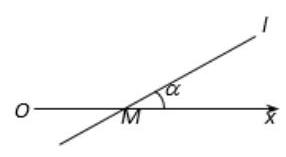
\includegraphics[max width=0.2\textwidth]{images/bo_d6dcisv7aajc739b5agg_40_888_1925_286_157_0.jpg}
\end{center}
\hspace*{3em} 

15. 三位同学参加跳高、跳远、铅球项目的比赛. 若每人都选择其中两个项目, 则有且仅有两人选择的项目完全相同的概率是\_\_\_\_\_(结果用最简分数表示).

16. 在平行四边形 \({ABCD}\) 中, \(\angle A = \frac{\pi }{3}\) ,边 \({AB},{AD}\) 的长分别为2,1. 若 \(M,N\) 分别是边 \({BC}\) ， \({CD}\) 上的点，且满足 \(\frac{\left| \overrightarrow{BM}\right| }{\left| \overrightarrow{BC}\right| } = \frac{\left| \overrightarrow{CN}\right| }{\left| \overrightarrow{CD}\right| }\) ，则 \(\overrightarrow{AM} \cdot  \overrightarrow{AN}\) 的取值范围是\_\_\_\_\_.

17. 已知函数 \(y = f\left( x\right)\) 的图像是折线段 \({ABC}\) ,若中 \(A\left( {0,0}\right) ,B\left( {\frac{1}{2},5}\right) ,C\left( {1,0}\right)\) . 函数 \(y = \; {xf}\left( x\right) \left( {0 \leq  x \leq  1}\right)\) 的图像与 \(x\) 轴围成的图形的面积为\_\_\_\_\_.

18. 如图, \({AD}\) 与 \({BC}\) 是四面体 \({ABCD}\) 中互相垂直的棱, \({BC} = 2\) . 若

\begin{center}
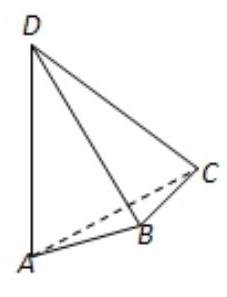
\includegraphics[max width=0.2\textwidth]{images/bo_d6dcisv7aajc739b5agg_41_1213_1592_227_297_0.jpg}
\end{center}
\hspace*{3em} 

\({AD} = \; {2c}\) ,且 \({AB} + {BD} = {AC} + {CD} = {2a}\) ,其中 \(a,c\) 为常数,则四面体 \({ABCD}\) 的体积的最大值是\_\_\_\_\_.

19. 如图,在四棱锥 \(P - {ABCD}\) 中,底面 \({ABCD}\) 是矩形, \({PA} \bot\) 底面 \({ABCD},E\) 是 \({PC}\) 的中

点. 已知 \({AB} = 2,{AD} = 2\sqrt{2},{PA} = 2\) . 求:

\begin{center}
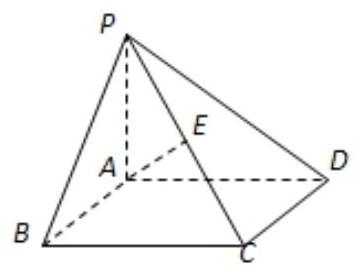
\includegraphics[max width=0.2\textwidth]{images/bo_d6dcisv7aajc739b5agg_42_954_471_356_269_0.jpg}
\end{center}
\hspace*{3em} 

(1)三角形 \({PCD}\) 的面积;

(2)异面直线 \({BC}\) 与 \({AE}\) 所成的角的大小.

20. 已知函数 \(f\left( x\right)  = \lg \left( {x + 1}\right)\) .

(1) 若 \(0 < f\left( {1 - {2x}}\right)  - f\left( x\right)  < 1\) ，求 \(x\) 的取值范围；

( 2 )若 \(g\left( x\right)\) 是以 2 为周期的偶函数，且当 \(0 \leq  x \leq  1\) 时，有 \(g\left( x\right)  = f\left( x\right)\) ，求函数 \(y = \; g\left( x\right) \left( {x \in  \left\lbrack  {1,2}\right\rbrack  }\right)\) 的反函数.

21. 海事救援船对一艘失事船进行定位:以失事船的当前位置为原点，以正北方向为 \(y\) 轴正方向建立平面直角坐标系 (以 1 海里为单位长度),则救援船恰在失事船的正南方向 12 海里 \(A\) 处, 如图. 现假设:

 \circled{1} 失事船的移动路径可视为抛物线 \(y = \frac{12}{49}{x}^{2}\) ;  \circled{2} 定位后救援船即刻沿直线匀速前往救援； \circled{3} 

救援船出发 \(t\) 小时后,失事船所在位置的横坐标为 \({7t}\) .

\begin{center}
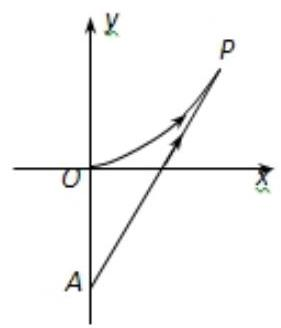
\includegraphics[max width=0.2\textwidth]{images/bo_d6dcisv7aajc739b5agg_43_1016_222_281_328_0.jpg}
\end{center}
\hspace*{3em} 

(1)当 \(t = {0.5}\) 时，写出失事船所在位置 \(P\) 的纵坐标. 若此时两船恰好会合，求救援船速度的大小和方向;

(2)问救援船的时速至少是多少海里才能追上失事船？

22. 在平面直角坐标系 \({xOy}\) 中,已知双曲线 \({C}_{1} : \;2{x}^{2} - {y}^{2} = 1\) .

(1)过 \({C}_{1}\) 的左顶点引 \({C}_{1}\) 的一条渐近线的平行线，求该直线与另一条渐近线及 \(x\) 轴围成的三角形的面积;

(2) 设斜率为 1 的直线 \(l\) 交 \({C}_{1}\) 于 \(P\text{ 、 }Q\) 两点,若 \(l\) 与圆 \({x}^{2} + {y}^{2} = 1\) 相切,求证: \({OP} \bot  {OQ}\) ;

(3)设椭圆 \({C}_{2} : 4{x}^{2} + {y}^{2} = 1\) . 若 \(M\text{ 、 }N\) 分别是 \({C}_{1}\text{ 、 }{C}_{2}\) 上的动点,且 \({OM} \bot  {ON}\) ,求证: \(O\) 到直线 \({MN}\) 的距离是定值.

23. 对于数集 \(X =  - 1,{x}_{1},{x}_{2},\cdots ,{x}_{n}\) ,其中 \(0 < {x}_{1} < {x}_{2} < \cdots  < {x}_{n},n \geq  2\) ,定义向量集 \(Y = \; \left\{  {\overrightarrow{a} \mid  \overrightarrow{a} = \left( {s,t}\right) ,s \in  X,t \in  X}\right\}\) . 若对于任意 \({\overrightarrow{a}}_{1} \in  Y\) ,存在 \({\overrightarrow{a}}_{2} \in  Y\) ,使得 \({\overrightarrow{a}}_{1} \cdot  {\overrightarrow{a}}_{2} = 0\) ,则称 \(X\) 具有性质 \(P\) . 例如 \(X = \{  - 1,1,2\}\) 具有性质 \(P\) .

(1) 若 \(x > 2\) ,且 \(\{  - 1,1,2,x\}\) ,求 \(x\) 的值;

( 2 )若 \(X\) 具有性质 \(P\) ，求证: \(1 \in  X\) ，且当 \({x}_{n} > 1\) 时， \({x}_{1} = 1\) ；

(3)若 \(X\) 具有性质 \(P\) ,且 \({x}_{1} = 1,{x}_{2} = q\) ( \(q\) 为常数),求有穷数列 \({x}_{1},{x}_{2},\cdots ,{x}_{n}\) 的通项公式.

一、填空题(本大题满分 56 分)本大题共有 14 题，要求直接填写结果，每题答对得 4 分， 否则一律得零分。

1. 已知集合 \(A = \{ 1,2,k\} ,B = \{ 2,5\}\) . 若 \(A \cup  B = \{ 1,2,3,5\}\) ，则 \(k =\) \_\_\_\_\_.

2. 函数 \(y = \sqrt{x + 2}\) 的定义域是\_\_\_\_\_.

3. 抛物线 \({y}^{2} = {8x}\) 的焦点坐标是\_\_\_\_\_.

4. 若复数 \(z\) 满足 \({iz} = 1 + \mathrm{i}\) ( \(\mathrm{i}\) 为虚数单位),则 \(z =\) \_\_\_\_\_.

5. 函数 \(f\left( x\right)  = \sin \left( {{2x} + \frac{\pi }{4}}\right)\) 的最小正周期为\_\_\_\_\_.

6. 方程 \({4}^{x} - {2}^{x + 1} = 0\) 的解为\_\_\_\_\_.

7. 若 \({\left( 2x - 1\right) }^{5} = {a}_{0} + {a}_{1}x + {a}_{2}{x}^{2} + {a}_{3}{x}^{3} + {a}_{4}{x}^{4} + {a}_{5}{x}^{5}\) ，则 \({a}_{0} + {a}_{1} + {a}_{2} + {a}_{3} + {a}_{4} + {a}_{5} =\) \_\_\_\_\_.

8. 若 \(f\left( x\right)  = \frac{\left( {x + 2}\right) \left( {x + m}\right) }{x}\) 为奇函数，则实数 \(m =\) \_\_\_\_\_.

9. 函数 \(y = {\log }_{2}x + \frac{4}{{\log }_{2}x}\left( {x \in  \left\lbrack  {2,4}\right\rbrack  }\right)\) 的最大值为\_\_\_\_\_.

10. 若复数 \(z\) 满足 \(\left| {z - \mathrm{i}}\right|  \leq  \sqrt{2}\) ( \(\mathrm{i}\) 为虚数单位),则 \(z\) 在复平面内所对应的图形的面积为\_\_\_\_\_.

11. 某校要从 2 名男生和 4 名女生中选出 4 人担任某游泳赛事的志愿者工作，则在选出的志愿者中，男、女生都有的概率为\_\_\_\_\_. (结果用数值表示)

12. 若不等式 \({x}^{2} - {kx} + k - 1 > 0\) 对 \(x \in  \left( {1,2}\right)\) 恒成立,则实数 \(k\) 的取值范围是\_\_\_\_\_.

13. 已知等差数列 \(\left\{  {a}_{n}\right\}\) 的首项及公差均为正数,令 \({b}_{n} = \sqrt{{a}_{n}} + \sqrt{{a}_{{2012} - n}}\left( {n \in  {N}^{ * },n < {2012}}\right)\) . 当 \({b}_{k}\) 是数列 \(\left\{  {b}_{n}\right\}\) 的最大项时, \(k =\) \_\_\_\_\_.

14. 若矩阵 \(\left\lbrack  \begin{array}{l} {a}_{11} \\  {a}_{21} \end{array}\right\rbrack\) 满足 \({a}_{11},{a}_{12},{a}_{21},{a}_{22} \in  \{  - 1,1\}\) ,且 \(\left| \begin{array}{l} {a}_{11} \\  {a}_{21} \end{array}\right|  = 0\) ,则这样的互不相等的矩阵共有\_\_\_\_\_个.

二、选择题 (本大题满分 20 分) 本大题共有 4 题，每题都给出四个结论，其中有且只有一个结论是正确的，选对得 5 分，否则一律得零分。

15. 已知椭圆 \({C}_{1} : \frac{{x}^{2}}{12} + \frac{{y}^{2}}{4} = 1,{C}_{2} : \frac{{x}^{2}}{16} + \frac{{y}^{2}}{8} = 1\) ,则 ( )

A. \({C}_{1}\) 与 \({C}_{2}\) 顶点相同 B. \({C}_{1}\) 与 \({C}_{2}\) 长轴长相同

C. \({C}_{1}\) 与 \({C}_{2}\) 短轴长相同 D. \({C}_{1}\) 与 \({C}_{2}\) 焦距相等

16. 记函数 \(y = f\left( x\right)\) 的反函数为 \(y = {f}^{-1}\left( x\right)\) . 如果函数 \(y = f\left( x\right)\) 的图象过点 \(\left( {1,0}\right)\) ,那么函数 \(y \; = {f}^{-1}\left( x\right)  + 1\) 的图象过点 ( )

A. \(\left( {0,0}\right)\) B. \(\left( {0,2}\right)\) C. \(\left( {1,1}\right)\) D. \(\left( {2,0}\right)\)

17. 已知空间三条直线 \(l\text{ 、 }m\text{ 、 }n\) . 若 \(l\) 与 \(m\) 异面,且 \(l\) 与 \(n\) 异面,则 ( )

A. \(m\) 与 \(n\) 异面 B. \(m\) 与 \(n\) 相交

C. \(m\) 与 \(n\) 平行 D. \(m\) 与 \(n\) 异面、相交、平行均有可能

18. 设 \(O\) 为 \(\bigtriangleup {ABC}\) 所在平面内一点. 若实数 \(x\text{ 、 }y\text{ 、 }z\) 满足 \(x\overrightarrow{OA} + y\overrightarrow{OB} + z\overrightarrow{OC} = \overrightarrow{0}\) , \(\left( {{x}^{2} + {y}^{2} + {z}^{2} \neq  0}\right)\) ,则 “ \({xyz} = 0\) ” 是 “点 \(O\) 在 \(\bigtriangleup {ABC}\) 的边所在直线上” 的 ( )

A. 充分而不必要条件 B. 必要而不充分条件

C. 充要条件 D. 既不充分也不必要条件

\section*{三、解答题(本大题满分 74 分)本大题共有 5 题，解答下列各题必须写出必要的步骤。}

19. 如图,正四棱柱 \({ABCD} - {A}_{1}{B}_{1}{C}_{1}{D}_{1}\) 的底面边长为 1,高为 2, \(M\) 为线段 \({AB}\) 的中点. 求:

\begin{center}
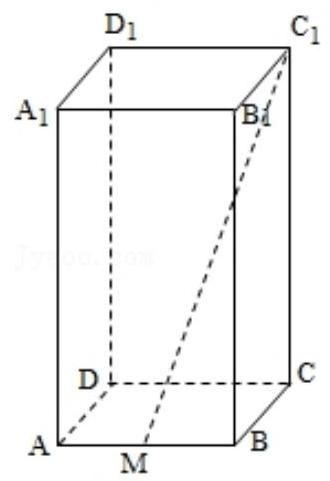
\includegraphics[max width=0.2\textwidth]{images/bo_d6dcisv7aajc739b5agg_47_281_1007_330_481_0.jpg}
\end{center}
\hspace*{3em} 

(1)三棱锥 \({C}_{1} - {MBC}\) 的体积；

(2)异面直线 \({CD}\) 与 \(M{C}_{1}\) 所成角的大小(结果用反三角函数值表示).

20. 某环线地铁按内、外环线同时运行，内、外环线的长均为 30 千米(忽略内、外环线长度差异).

(1)当 9 列列车同时在内环线上运行时，要使内环线乘客最长候车时间为 10 分钟，求内环线列车的最小平均速度;

(2)新调整的方案要求内环线列车平均速度为 25 千米/小时，外环线列车平均速度为 30 千米/

小时. 现内、外环线共有 18 列列车全部投入运行, 要使内外环线乘客的最长候车时间之差不超过 1 分钟, 向内、外环线应各投入几列列车运行?

21. 已知双曲线 \({C}_{1} : \;{x}^{2} - \frac{{y}^{2}}{4} = 1\) .

(1)求与双曲线 \({C}_{1}\) 有相同焦点，且过点 \(P\left( {4,\sqrt{3}}\right)\) 的双曲线 \({C}_{2}\) 的标准方程；

(2)直线 \(l : y = x + m\) 分别交双曲线 \({C}_{1}\) 的两条渐近线于 \(A\text{ 、 }B\) 两点. 当 \(\overrightarrow{OA}\overrightarrow{OB} = 3\) 时,求实数 \(m\) 的值.

22. 已知数列 \(\left\{  {a}_{n}\right\}\) 、 \(\left\{  {b}_{n}\right\}\) 、 \(\left\{  {c}_{n}\right\}\) 满足 \(\left( {{a}_{n + 1} - {a}_{n}}\right) \left( {{b}_{n + 1} - {b}_{n}}\right)  = {c}_{n}\left( {n \in  {N}^{ * }}\right)\) .

(1)设 \({c}_{n} = {3n} + 6\) ， \(\left\{  {a}_{n}\right\}\) 是公差为3的等差数列. 当 \({b}_{1} = 1\) 时，求 \({b}_{2}\) 、 \({b}_{3}\) 的值；

(2)设 \({c}_{n} = {n}^{3},{a}_{n} = {n}^{2} - {8n}\) . 求正整数 \(k\) ，使得对一切 \(n \in  {N}^{ * }\) ，均有 \({b}_{n} \geq  {b}_{k}\) ；

23. 定义向量 \(\overrightarrow{OM} = \left( {a,b}\right)\) 的 “相伴函数” 为 \(f\left( x\right)  = a\sin x + b\cos x\) ,函数 \(f\left( x\right)  = a\sin x + \; b\cos x\) 的 “相伴向量” 为 \(\overrightarrow{OM} = \left( {a,b}\right)\) (其中 \(O\) 为坐标原点). 记平面内所有向量的 “相伴函数” 构成的集合为 \(S\) .

(1)设 \(g\left( x\right)  = 3\sin \left( {x + \frac{\pi }{2}}\right)  + 4\sin x\) ，求证: \(g\left( x\right)  \in  S\) ；

( 2 )已知 \(h\left( x\right)  = \cos \left( {x + \alpha }\right)  + 2\cos x\) ，且 \(h\left( x\right)  \in  S\) ，求其 “相伴向量” 的模；

24. \(\operatorname{an}2{x}_{0} = \frac{2\tan {x}_{0}}{1 - {\tan }^{2}{x}_{0}} = \frac{2 \times  \frac{a}{b}}{1 - {\left( \frac{a}{b}\right) }^{2}} = \frac{2}{\frac{b}{a} - \frac{a}{b}}\) .

\(\frac{b}{a}\) 为直线 \({OM}\) 的斜率,由几何意义知: \(\frac{b}{a} \in  \left\lbrack  {-\frac{\sqrt{3}}{3},0}\right)  \cup  \left( {0,\frac{\sqrt{3}}{3}}\right\rbrack\) .

令 \(m = \frac{b}{a}\) ,则 \(\tan 2{x}_{0} = \frac{2}{m - \frac{1}{m}},m \in  \left\lbrack  {-\frac{\sqrt{3}}{3},0}\right)  \cup  \left( {0,\frac{\sqrt{3}}{3}}\right\}\) .

当 \(- \frac{\sqrt{3}}{3} \leq  m < 0\) 时,函数 \(\tan 2{x}_{0} = \frac{2}{m - \frac{1}{m}}\) 单调递减, \(\therefore 0 < \tan 2{x}_{0} \leq  \sqrt{3}\) ;

当 \(0 < m \leq  \frac{\sqrt{3}}{3}\) 时,函数 \(\tan 2{x}_{0} = \frac{2}{m - \frac{1}{m}}\) 单调递减, \(\therefore  - \sqrt{3} \leq  \tan 2{x}_{0} < 0\) .

综上所述， \(\tan 2{x}_{0} \in  \left\lbrack  {-\sqrt{3},0}\right)  \cup  \left( {0,\sqrt{3}}\right\rbrack\) .

\section*{2013 秋考}

\section*{填空}

1. 计算: \(\mathop{\lim }\limits_{{n \rightarrow  \infty }}\frac{n + {20}}{{3n} + {13}} =\) \_\_\_\_\_.

2. 设 \(m \in  R,{m}^{2} + m - 2 + \left( {{m}^{2} - 1}\right) \mathrm{i}\) 是纯虚数,其中 \(\mathrm{i}\) 是虚数单位,则 \(m =\) \_\_\_\_\_.

3. 若 \(\left| \begin{matrix} {x}^{2} & {y}^{2} \\   - 1 & 1 \end{matrix}\right|  = \left| \begin{matrix} x & x \\  y &  - y \end{matrix}\right|\) ,则 \(x + y =\) \_\_\_\_\_.

4. 已知 \({ABC}\) 的内角 \(A,B,C\) 所对应边分别为 \(a,b,c\) ,若 \(3{a}^{2} + {2ab} + 3{b}^{2} - 3{c}^{2} = 0\) ,则角 \(C\) 的大小是\_\_\_\_\_ (结果用反三角函数值表示).

5. 设常数 \(a \in  R\) . 若 \({\left( {x}^{2} + \frac{a}{x}\right) }^{5}\) 的二项展开式中 \({x}^{7}\) 项的系数为 -10,则 \(a =\) \_\_\_\_\_.

6. 方程 \(\frac{3}{{3}^{x} - 1} + \frac{1}{3} = {3}^{x - 1}\) 的实数解为\_\_\_\_\_.

7. 在极坐标系中，曲线 \(\rho  = \cos \theta  + 1\) 与 \(\rho \cos \theta  = 1\) 的公共点到极点的距离为\_\_\_\_\_.

8. 盒子中装有编号为1,2,3,4,5,6,7,8,9的九个球,从中任意取出两个,则这两个球的编号之积为偶数的概率是\_\_\_\_\_(结果用最简分数表示).

9. 设 \({AB}\) 是椭圆 \(\Gamma\) 的长轴,点 \(C\) 在 \(\Gamma\) 上,且 \(\angle {CBA} = \frac{\pi }{4}\) . 若 \({AB} = 4,{BC} = \sqrt{2}\) ,则 \(\Gamma\) 的两个焦点之间的距离为\_\_\_\_\_.

10. 设非零常数 \(d\) 是等差数列 \({x}_{1},{x}_{2},{x}_{3},\cdots ,{x}_{19}\) 的公差,随机变量 \(\xi\) 等可能地取值 \({x}_{1},{x}_{2}\) , \({x}_{3},\cdots ,{x}_{19}\) ,则方差 \({D\xi } =\) \_\_\_\_\_.

11. 若 \(\cos x\cos y + \sin x\sin y = \frac{1}{2},\sin {2x} + \sin {2y} = \frac{2}{3}\) ,则 \(\sin \left( {x + y}\right)  =\) \_\_\_\_\_.

12. 设 \(a\) 为实常数, \(y = f\left( x\right)\) 是定义在 \(R\) 上的奇函数,当 \(x < 0\) 时, \(f\left( x\right)  = {9x} + \frac{{a}^{2}}{x} + 7\) ,若 \(f\left( x\right)  \geq  a + 1\) 对一切 \(x \geq  0\) 成立,则 \(a\) 的取值范围为\_\_\_\_\_.

13. 在 \({xOy}\) 平面上,将两个半圆弧 \({\left( x - 1\right) }^{2} + {y}^{2} = 1\left( {x \geq  1}\right)\) 和 \({\left( x - 3\right) }^{2} + {y}^{2} = 1\left( {x \geq  3}\right)\) 、两条直线 \(y = 1\) 和 \(y =  - 1\) 围成的封闭图形记为 \(D\) ,如图中阴影部分. 记 \(D\) 绕 \(y\) 轴旋转一周而成的几何体为 \(\Omega\) ,过 \(\left( {0,y}\right) \left( {\left| y\right|  \leq  1}\right)\) 作 \(\Omega\) 的水平截面,所得截面面积为 \({4\pi }\sqrt{1 - {y}^{2}} + {8\pi }\) ,试利用祖暅原理、一个平放的圆柱和一个长方体，得出 \(\Omega\) 的体积值为\_\_\_\_\_.

\begin{center}
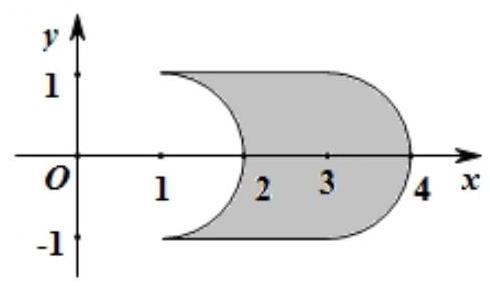
\includegraphics[max width=0.3\textwidth]{images/bo_d6dcisv7aajc739b5agg_51_303_1446_490_286_0.jpg}
\end{center}
\hspace*{3em} 

14. 对区间 \(I\) 上有定义的函数 \(g\left( x\right)\) ,记 \(g\left( I\right)  = \{ y \mid  y = g\left( x\right) ,x \in  I\}\) ,已知定义域为 \(\left\lbrack  {0,3}\right\rbrack\) 的函数 \(y \; = f\left( x\right)\) 有反函数 \(y = {f}^{-1}\left( x\right)\) ,且 \({f}^{-1}\left( {\lbrack 0,1}\right) ) = \lbrack 1,2),{f}^{-1}\left( {(2,4\rbrack }\right)  = \lbrack 0,1)\) ,若方程 \(f\left( x\right)  - x \; = 0\) 有解 \({x}_{0}\) ,则 \({x}_{0} =\) \_\_\_\_\_.

15. 设常数 \(a \in  R\) ,集合 \(A = \{ x \mid  \left( {x - 1}\right) \left( {x - a}\right)  \geq  0\} ,B = \{ x \mid  x \geq  a - 1\}\) . 若 \(A \cup  B = R\) ,则 \(a\) 的取值范围为 ( ).

A. \(\left( {-\infty ,2}\right)\) B. \(\left( {-\infty ,2}\right)\) C. \(\left( {2, + \infty }\right)\) D. \(\lbrack 2, + \infty )\)

16. 钱大姐常说 “便宜没好货”，她这句话的意思是:“不便宜”是 “好货” 的()

A. 充要条件 B. 既不充分也不必要条件

C. 充分条件 D. 必要条件

17. 在数列 \(\left\{  {a}_{n}\right\}\) 中, \({a}_{n} = {2}^{n} - 1\) ,若一个 7 行 12 的矩阵的第 \(\mathrm{i}\) 行第 \(j\) 列的元素 \({a}_{i,j} = {a}_{i} \cdot  {a}_{j} + {a}_{i} + \; {a}_{j},\;\left( {\mathrm{i} = 1,2,\cdots ,{71};j = 1,2,\cdots ,{12}}\right)\) 则该矩阵元素能取到的不同数值的个数为 ( )

A. 18 B. 28 C. 48 D. 63

18. 在边长为 1 的正六边形 \({ABCDEF}\) 中,记以 \(A\) 为起点,其余顶点为终点的向量分别为 \({\overrightarrow{a}}_{1}\) , \({\overrightarrow{a}}_{2},{\overrightarrow{a}}_{3},{\overrightarrow{a}}_{4},{\overrightarrow{a}}_{5}\) ; 以 \(D\) 为起点,其余顶点为终点的向量分别为 \({\overrightarrow{d}}_{1},{\overrightarrow{d}}_{2},{\overrightarrow{d}}_{3},{\overrightarrow{d}}_{4},{\overrightarrow{d}}_{5}\) . 若 \(m,M\) 分别为 \(\left( {{\overrightarrow{a}}_{i} + {\overrightarrow{a}}_{j} + {\overrightarrow{a}}_{k}}\right)  \cdot  \left( {{\overrightarrow{d}}_{r} + {\overrightarrow{d}}_{s} + {\overrightarrow{d}}_{t}}\right)\) 的最小值、最大值,其中 \(\{ \mathrm{i},j,k\}  \subseteq  \{ 1,2,3,4,5\}\) , \(\{ r,s,t\}  \subseteq  \{ 1,2,3,4,5\}\) ,则 \(m,M\) 满足 ().

A. \(m = 0,M > 0\) B. \(m < 0,M > 0\) C. \(m < 0,M = 0\) D. \(m < 0,M < 0\)

19. 如图，在长方体 \({ABCD} - {A}_{1}{B}_{1}{C}_{1}{D}_{1}\) 中， \({AB} = 2,{AD} = 1,{A}_{1}A = 1\) ，

\begin{center}
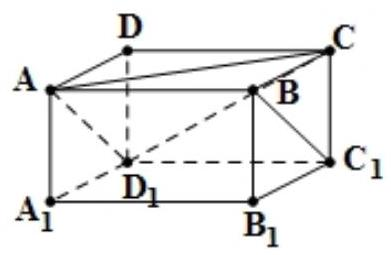
\includegraphics[max width=0.3\textwidth]{images/bo_d6dcisv7aajc739b5agg_53_329_471_391_255_0.jpg}
\end{center}
\hspace*{3em} 

20. 甲厂以 \(x\) 千克/小时的速度运输生产某种产品 (生产条件要求 \(1 \leq  x \leq  {10}\) ),每小时可获得利润是 \({100}\left( {{5x} + 1 - \frac{3}{x}}\right)\) 元.

(1)要使生产该产品 2 小时获得的利润不低于 3000 元，求 \(x\) 的取值范围；

(2)要使生产 900 千克该产品获得的利润最大，问:甲厂应该选取何种生产速度？并求最大利润.

21. 已知函数 \(f\left( x\right)  = 2\sin \left( {\omega x}\right)\) ,其中常数 \(\omega  > 0\) .

(1)若 \(y = f\left( x\right)\) 在 \(\left\lbrack  {-\frac{\pi }{4},\frac{2\pi }{3}}\right\rbrack\) 上单调递增，求 \(\omega\) 的取值范围；

( 2 )令 \(\omega  = 2\) ，将函数 \(y = f\left( x\right)\) 的图象向左平移 \(\frac{\pi }{6}\) 个单位，再向上平移 1 个单位，得到函数 \(y = \; g\left( x\right)\) 的图象,区间 \(\left\lbrack  {a,b}\right\rbrack  \left( {a,b \in  R\text{ 且 }a < b}\right)\) 满足: \(y = g\left( x\right)\) 在 \(\left\lbrack  {a,b}\right\rbrack\) 上至少含有 30 个零点, 在所有满足上述条件的 \(\left\lbrack  {a,b}\right\rbrack\) 中,求 \(b - a\) 的最小值.

22. 如图,已知曲线 \({C}_{1} : \frac{{x}^{2}}{2} - {y}^{2} = 1\) ,曲线 \({C}_{2} : \left| y\right|  = \left| x\right|  + 1,P\) 是平面上一点,若存在过点 \(P\)

的直线与 \({C}_{1},{C}_{2}\) 都有公共点,则称 \(P\) 为 “ \({C}_{1} - {C}_{2}\) 型点”.

\begin{center}
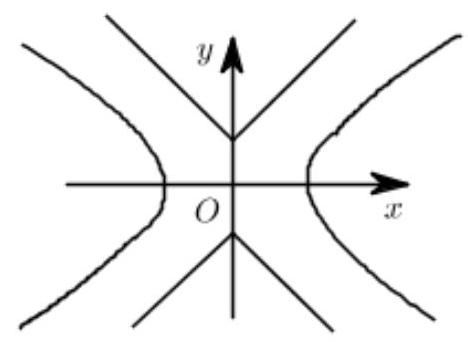
\includegraphics[max width=0.3\textwidth]{images/bo_d6dcisv7aajc739b5agg_54_265_274_468_342_0.jpg}
\end{center}
\hspace*{3em} 

(1)在正确证明 \({C}_{1}\) 的左焦点是 \({}^{c}{C}_{1} - {C}_{2}\) 型点” 时，要使用一条过该焦点的直线，试写出一条这样的直线的方程 (不要求验证);

(2)设直线 \(y = {kx}\) 与 \({C}_{2}\) 有公共点，求证 \(\left| k\right|  > 1\) ，进而证明原点不是 “ \({C}_{1} - {C}_{2}\) 型点”；

23. 给定常数 \(c > 0\) ,定义函数 \(f\left( x\right)  = 2\left| {x + c + 4}\right|  - \left| {x + c}\right|\) ,数列 \({a}_{1},{a}_{2},{a}_{3},\cdots\) 满足 \({a}_{n + 1} = \; f\left( {a}_{n}\right) ,\;n \in  {N}^{ * }.\)

(1) 若 \({a}_{1} =  - c - 2\) ，求 \({a}_{2}\) 及 \({a}_{3}\) ；

(2)求证:对任意 \(n \in  {N}^{ * }\) ， \({a}_{n + 1} - {a}_{n} \geq  c\) ；

\section*{2013 春考}

一、填空题(本大题满分 36 分)本大题共有 12 题，要求直接填写结果，每题填对得 3 分， 否则一律得 0 分.

1. 函数 \(y = {\log }_{2}\left( {x + 2}\right)\) 的定义域是\_\_\_\_\_.

2. 方程 \({2}^{x} = 8\) 的解是\_\_\_\_\_.

3. 抛物线 \({y}^{2} = {8x}\) 的准线方程是\_\_\_\_\_.

4. 函数 \(y = 2\sin x\) 的最小正周期是\_\_\_\_\_.

5. 已知向量 \(\overrightarrow{a} = \left( {1,k}\right) ,\overrightarrow{b} = \left( {9,k - 6}\right)\) . 若 \(\overrightarrow{a}//\overrightarrow{b}\) ，则实数 \(k =\) \_\_\_\_\_.

6. 函数 \(y = 4\sin x + 3\cos x\) 的最大值是\_\_\_\_\_.

7. 复数 \(2 + 3\mathrm{i}\) ( \(\mathrm{i}\) 是虚数单位) 的模是\_\_\_\_\_.

8. 在 \(\bigtriangleup {ABC}\) 中,角 \(A,B,C\) 所对边长分别为 \(a,b,c\) ,若 \(a = 5,c = 8,B = {60}\) 。,则 \(b =\) \_\_\_\_\_.

9. 正方体 \({ABCD} - {A}_{1}{B}_{1}{C}_{1}{D}_{1}\) 中，异面直线 \({A}_{1}B\) 与 \({B}_{1}C\) 所成角的大小为\_\_\_\_\_.

\begin{center}
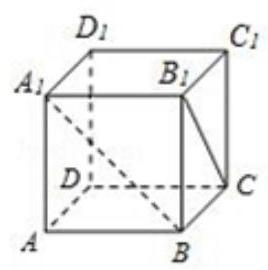
\includegraphics[max width=0.2\textwidth]{images/bo_d6dcisv7aajc739b5agg_56_277_504_268_270_0.jpg}
\end{center}
\hspace*{3em} 

10. 从 4 名男同学和 6 名女同学中随机选取 3 人参加某社团活动, 选出的 3 人中男女同学都有的概率为\_\_\_\_\_ (结果用数值表示).

11. 若等差数列的前 6 项和为 23 , 前 9 项和为 57 , 则数列的前 \(n\) 项和 \({S}_{n} =\) \_\_\_\_\_.

12.36 的所有正约数之和可按如下方法得到: 因为 \({36} = {2}^{2} \times  {3}^{2}\) ,所以 36 的所有正约数之和为 \(\left( {1 + 3 + {3}^{2}}\right)  + \left( {2 + 2 \times  3 + 2 \times  {3}^{2}}\right)  + \left( {{2}^{2} + {2}^{2} \times  3 + {2}^{2} \times  {3}^{2}}\right)  = \left( {1 + 2 + {2}^{2}}\right) \left( {1 + 3 + {3}^{2}}\right)  = {91}\) ,参照上述方法, 可求得 2000 的所有正约数之和为\_\_\_\_\_.

二. 选择题 (本大题满分 36 分) 本大题共有 12 题, 每题都给出四个结论, 其中有且只有一

个结论是正确的. 考生必须把真确结论的代码写在题后的括号内, 选对得 3 分, 否则一律得 0 分.

13. 展开式为 \({ad} - {bc}\) 的行列式是 ( )

A. \(\left| \begin{array}{l} a \\  d \end{array}\right|\) B. \(\left| \begin{array}{l} a \\  b \end{array}\right|\) C. \(\left| \begin{array}{l} a \\  b \end{array}\right|\) D. \(\left| \begin{array}{l} b \\  d \end{array}\right|\)

14. 设 \({f}^{-1}\left( x\right)\) 为函数 \(f\left( x\right)  = \sqrt{x}\) 的反函数,下列结论正确的是 ( )

A. \({f}^{-1}\left( 2\right)  = 2\) B. \({f}^{-1}\left( 2\right)  = 4\) C. \({f}^{-1}\left( 4\right)  = 2\) D. \({f}^{-1}\left( 4\right)  = 4\)

15. 直线 \({2x} - {3y} + 1 = 0\) 的一个方向向量是 ( )

A. \(\left( {2, - 3}\right)\) B. \(\left( {2,3}\right)\) C. \(\left( {-3,2}\right)\) D. \(\left( {3,2}\right)\)

16. 函数 \(f\left( x\right)  = {x}^{-\frac{1}{2}}\) 的大致图象是 ( )

A.

\begin{center}
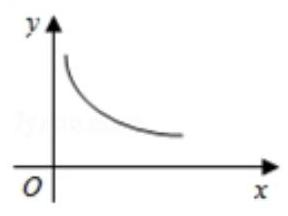
\includegraphics[max width=0.2\textwidth]{images/bo_d6dcisv7aajc739b5agg_57_362_1558_288_216_0.jpg}
\end{center}
\hspace*{3em} 

B.

\begin{center}
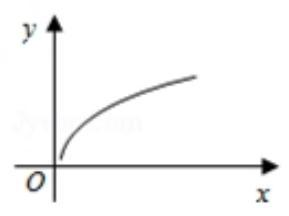
\includegraphics[max width=0.2\textwidth]{images/bo_d6dcisv7aajc739b5agg_57_944_1552_289_216_0.jpg}
\end{center}
\hspace*{3em} 

C.

\begin{center}
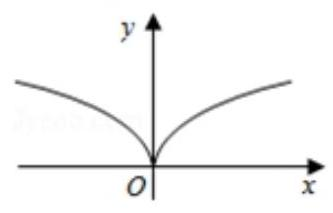
\includegraphics[max width=0.2\textwidth]{images/bo_d6dcisv7aajc739b5agg_57_362_1793_333_213_0.jpg}
\end{center}
\hspace*{3em} 

D.

\begin{center}
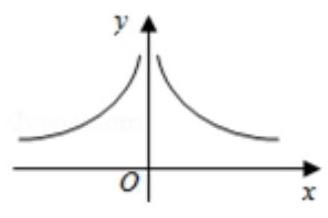
\includegraphics[max width=0.2\textwidth]{images/bo_d6dcisv7aajc739b5agg_57_939_1791_328_218_0.jpg}
\end{center}
\hspace*{3em} 

17. 如果 \(a < b < 0\) ,那么下列不等式成立的是 ( )

A. \(\frac{1}{a} < \frac{1}{b}\) B. \({ab} < {b}^{2}\) C. \(- {ab} <  - {a}^{2}\) D. \(- \frac{1}{a} <  - \frac{1}{b}\)

18. 若复数 \({z}_{1},{z}_{2}\) 满足 \({z}_{1} = {\bar{z}}_{2}\) ,则 \({z}_{1},{z}_{2}\) 在复数平面上对应的点 \({Z}_{1},{Z}_{2}\) ( )

A. 关于 \(x\) 轴对称 B. 关于 \(y\) 轴对称 C. 关于原点对称 D. 关于直线 \(y = x\) 对称

19. \({\left( 1 + x\right) }^{10}\) 的二项展开式中的一项是 ( )

A. \({45x}\) B. \({90}{x}^{2}\) C. \({120}{x}^{3}\) D. \({252}{x}^{4}\)

20. 既是偶函数又在区间 \(\left( {0,\pi }\right)\) 上单调递减的函数是 ( )

A. \(y = \sin x\) B. \(y = \cos x\) C. \(y = \sin {2x}\) D. \(y = \cos {2x}\)

21. 若两个球的表面积之比为1:4, 则这两个球的体积之比为 ( )

A. 1:2 B. 1:4 C. 1:8 D. 1:16

22. 设全集 \(U = R\) ,下列集合运算结果为 \(R\) 的是 ( )

A. \(Z \cup  {\complement }_{U}N\) B. \(N \cap  {\complement }_{U}N\) C. \({\complement }_{U}\left( {{\complement }_{U}\varnothing }\right)\) D. \({\complement }_{U}\{ 0\}\)

23. 已知 \(a,b,c \in  R\) ,“ \({b}^{2} - {4ac} < 0\) ” 是 “函数 \(f\left( x\right)  = a{x}^{2} + {bx} + c\) 的图象恒在 \(x\) 轴上方” 的 ( )

A. 充分非必要条件 B. 必要非充分条件

C. 充要条件 D. 既非充分又非必要条件

24. 已知 \(A,B\) 为平面内两个定点,过该平面内动点 \(m\) 作直线 \({AB}\) 的垂线,垂足为 \(N\) . 若 \({\overrightarrow{MN}}^{2} \; = \lambda \overrightarrow{AN} \cdot  \overrightarrow{NB}\) ,其中 \(\lambda\) 为常数,则动点 \(M\) 的轨迹不可能是 ( )

A. 圆 B. 椭圆 C. 双曲线 D. 抛物线

三、解答题 (本大题满分 78 分) 本大题共有 7 题, 解答下列各题必须写出必要的步骤.

25. 如图,在正三棱柱 \({ABC} - {A}_{1}{B}_{1}{C}_{1}\) 中， \({A{A}_{1}} = 6\) ，异面直线 \(B{C}_{1}\) 与 \(A{A}_{1}\) 所成角的大小为 \(\frac{\pi }{6}\) ， 求该三棱柱的体积.

\begin{center}
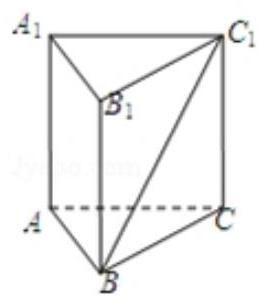
\includegraphics[max width=0.2\textwidth]{images/bo_d6dcisv7aajc739b5agg_60_261_232_262_301_0.jpg}
\end{center}
\hspace*{3em} 

26. 如图,某校有一块形如直角三角形 \({ABC}\) 的空地,其中 \(\angle B\) 为直角, \({AB}\) 长 40 米, \({BC}\) 长 50 米,现欲在此空地上建造一间健身房,其占地形状为矩形,且 \(B\) 为矩形的一个顶点,求该健身房的最大占地面积.

\begin{center}
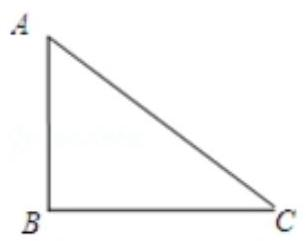
\includegraphics[max width=0.2\textwidth]{images/bo_d6dcisv7aajc739b5agg_60_265_940_306_241_0.jpg}
\end{center}
\hspace*{3em} 

27. 已知数列 \(\left\{  {a}_{n}\right\}\) 的前 \(n\) 项和为 \({S}_{n} =  - {n}^{2} + n\) ,数列 \(\left\{  {b}_{n}\right\}\) 满足 \({b}_{n} = {2}^{{a}_{n}}\) ,求 \(\mathop{\lim }\limits_{{n \rightarrow  \infty }}\left( {{b}_{1} + {b}_{2} + \cdots  + {b}_{n}}\right) .\)

28. 已知椭圆 \(C\) 的两个焦点分别为 \({F}_{1}\left( {-1,0}\right) \text{ 、 }{F}_{2}\left( {1,0}\right)\) ,短轴的两个端点分别为 \({B}_{1},{B}_{2}\) .

(1)若 \(\bigtriangleup {F}_{1}{B}_{1}{B}_{2}\) 为等边三角形，求椭圆 \(C\) 的方程；

(2)若椭圆 \(C\) 的短轴长为 2，过点 \({F}_{2}\) 的直线 \(l\) 与椭圆 \(C\) 相交于 \(P,Q\) 两点，且 \(\overrightarrow{{F}_{1}P} \bot  \overrightarrow{{F}_{1}Q}\) ，求直线 \(l\) 的方程.

29. 已知抛物线 \(C : {y}^{2} = {4x}\) 的焦点为 \(F\) .

(1) 点 \(A,P\) 满足 \(\overrightarrow{AP} =  - 2\overrightarrow{FA}\) . 当点 \(A\) 在抛物线 \(C\) 上运动时,求动点 \(P\) 的轨迹方程;

(2) 在 \(x\) 轴上是否存在点 \(Q\) ,使得点 \(Q\) 关于直线 \(y = {2x}\) 的对称点在抛物线 \(C\) 上? 如果存在,求所有满足条件的点 \(Q\) 的坐标; 如果不存在,请说明理由.

30. 在平面直角坐标系 \({xOy}\) 中,点 \(A\) 在 \(y\) 轴正半轴上,点 \({P}_{n}\) 在 \(x\) 轴上,其横坐标为 \({x}_{n}\) ,且 \(\left\{  {x}_{n}\right\}\) 是首项为 1、公比为 2 的等比数列,记 \(\angle {P}_{n}A{P}_{n + 1} = {\theta }_{n},n \in  {N}^{ * }\) .

\begin{center}
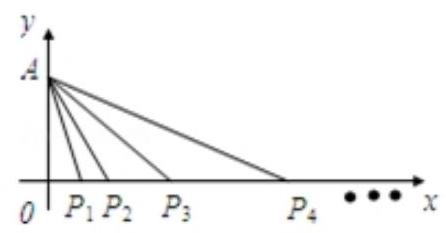
\includegraphics[max width=0.3\textwidth]{images/bo_d6dcisv7aajc739b5agg_61_266_759_446_233_0.jpg}
\end{center}
\hspace*{3em} 

(1)若 \({\theta }_{3} = \arctan \frac{1}{3}\) ，求点 \(A\) 的坐标；

(2)若点 \(A\) 的坐标为 \(\left( {0,8\sqrt{2}}\right)\) ，求 \({\theta }_{n}\) 的最大值及相应 \(n\) 的值.

31. 已知真命题: “函数 \(y = f\left( x\right)\) 的图象关于点 \(P\left( {a,b}\right)\) 成中心对称图形” 的充要条件为 “函数 \(y = f\left( {x + a}\right)  - b\) 是奇函数”.

(1)将函数 \(g\left( x\right)  = {x}^{3} - 3{x}^{2}\) 的图象向左平移 1 个单位，再向上平移 2 个单位，求此时图象对应的函数解析式,并利用题设中的真命题求函数 \(g\left( x\right)\) 图象对称中心的坐标;

(2)求函数 \(h\left( x\right)  = {\log }_{2}\frac{2x}{4 - x}\) 图象对称中心的坐标；

\section*{2014 秋考}

\section*{填空}

1. 函数 \(y = 1 - 2{\cos }^{2}\left( {2x}\right)\) 的最小正周期是\_\_\_\_\_.

2. 若复数 \(z = 1 + 2\mathrm{i}\) ，其中 \(\mathrm{i}\) 是虚数单位，则 \(\left( {z + \frac{1}{\bar{z}}}\right)  \cdot  \bar{z} =\) \_\_\_\_\_.

3. 若抛物线 \({y}^{2} = {2px}\) 的焦点与椭圆 \(\frac{{x}^{2}}{9} + \frac{{y}^{2}}{5} = 1\) 的右焦点重合，则该抛物线的准线方程为\_\_\_\_\_.

4. 设 \(f\left( x\right)  = \left\{  \begin{array}{l} x, \\  {x}^{2}, \end{array}\right.\) ，若 \(f\left( 2\right)  = 4\) ，则 \(a\) 的取值范围为\_\_\_\_\_.

5. 若实数 \(x,y\) 满足 \({xy} = 1\) ，则 \({x}^{2} + 2{y}^{2}\) 的最小值为\_\_\_\_\_.

6. 若圆锥的侧面积是底面积的 3 倍, 则其母线与底面角的大小为\_\_\_\_\_(结果用反三角函数值表示).

7. 已知曲线 \(C\) 的极坐标方程为 \(\rho \left( {3\cos \theta  - 4\sin \theta }\right)  = 1\) ,则 \(C\) 与极轴的交点到极点的距离是\_\_\_\_\_.

8. 设无穷等比数列 \(\left\{  {a}_{n}\right\}\) 的公比为 \(q\) ,若 \({a}_{1} = \mathop{\lim }\limits_{{n\infty }}\left( {{a}_{3} + {a}_{4} + \cdots  + {a}_{n}}\right)\) ,则 \(q =\) \_\_\_\_\_.

9. 若 \(f\left( x\right)  = {x}^{\frac{2}{3}} - {x}^{-\frac{1}{2}}\) ，则满足 \(f\left( x\right)  < 0\) 的 \(x\) 的取值范围是\_\_\_\_\_.

10. 为强化安全意识，某商场拟在未来的连续 10 天中随机选择 3 天进行紧急疏散演练，则选择的 3 天恰好为连续 3 天的概率是\_\_\_\_\_(结果用最简分数表示).

11. 已知互异的复数 \(a,b\) 满足 \({ab} \neq  0\) ，集合 \(\{ a,b\}  = \left\{  {{a}^{2},{b}^{2}}\right\}\) ，则 \(a + b =\) \_\_\_\_\_.

12. 设常数 \(a\) 使方程 \(\sin x + \sqrt{3}\cos x = a\) 在闭区间 \(\left\lbrack  {0,{2\pi }}\right\rbrack\) 上恰有三个解 \({x}_{1},{x}_{2},{x}_{3}\) ,则 \({x}_{1} + {x}_{2} \; + {x}_{3} =\) \_\_\_\_\_.

13. 某游戏的得分为1,2,3,4,5,随机变量 \(\xi\) 表示小白玩游戏的得分. 若 \(E\left( \xi \right)  = {4.2}\) ,则小白得 5 分的概率至少为\_\_\_\_\_.

14. 已知曲线 \(C : x =  - \sqrt{4 - {y}^{2}}\) ,直线 \(l : x = 6\) . 若对于点 \(A\left( {m,0}\right)\) ,存在 \(C\) 上的点 \(P\) 和 \(l\) 上的点 \(Q\) 使得 \(\overrightarrow{AP} + \overrightarrow{AQ} = \overrightarrow{0}\) ，则 \(m\) 的取值范围为\_\_\_\_\_.

15. 设 \(a,b \in  R\) ,则 “ \(a + b > 4\) ” 是 “ \(a > 2\) 且 \(b > 2\) ” 的( )

A. 充分条件 B. 必要条件

C. 充分必要条件 D. 既非充分又非必要条件

16. 如图,四个棱长为 1 的正方体排成一个正四棱柱, \({AB}\) 是一条侧棱, \({P}_{i}\left( {\mathrm{i} = 1,2,\cdots ,8}\right)\) 是上底面上其余的八个点,则 \(\overrightarrow{AB} \cdot  \overrightarrow{A{P}_{i}}\left( {\mathrm{i} = 1,2,\cdots ,8}\right)\) 的不同值的个数为 ().

\begin{center}
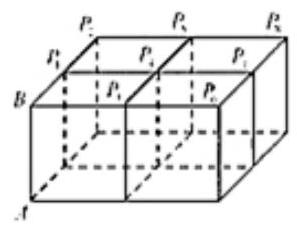
\includegraphics[max width=0.2\textwidth]{images/bo_d6dcisv7aajc739b5agg_64_255_1409_297_227_0.jpg}
\end{center}
\hspace*{3em} 

A. 1 B. 2 C. 4 D. 8

17. 已知 \({P}_{1}\left( {{a}_{1},{b}_{1}}\right)\) 与 \({P}_{2}\left( {{a}_{2},{b}_{2}}\right)\) 是直线 \(y = {kx} + 1\left( {k\text{ 为常数 }}\right)\) 上两个不同的点,则关于 \(x\) 和 \(y\) 的方程组 \(\left\{  \begin{array}{l} {a}_{1}x + {b}_{1}y = 1 \\  {a}_{2}x + {b}_{2}y = 1 \end{array}\right.\) ,的解的情况是 ().

A. 无论 \(k,{P}_{1},{P}_{2}\) 如何,总是无解 B. 无论 \(k,{P}_{1},{P}_{2}\) 如何,总有唯一解

C. 存在 \(k,{P}_{1},{P}_{2}\) ,使之恰有两解 D. 存在 \(k,{P}_{1},{P}_{2}\) ,使之有无穷多解

18. 设 \(f\left( x\right)  = \left\{  \begin{array}{l} {\left( x - a\right) }^{2}, \\  x + \frac{1}{x} + a, \end{array}\right.\) ,若 \(f\left( 0\right)\) 是 \(f\left( x\right)\) 的最小值,则 \(a\) 的取值范围为(   )

A. \(\left\lbrack  {-1,2}\right\rbrack\) B. \(\left\lbrack  {-1,0}\right\rbrack\) C. \(\left\lbrack  {1,2}\right\rbrack\) D. \(\left\lbrack  {0,2}\right\rbrack\)

19. 底面边长为 2 的正三棱锥 \(P - {ABC}\) ,其表面展开图是三角形 \({P}_{1}{P}_{2}{P}_{3}\) ,如图,求 \({P}_{1}{P}_{2}{P}_{3}\) 的各边长及此三棱锥的体积 \(V\) .

\begin{center}
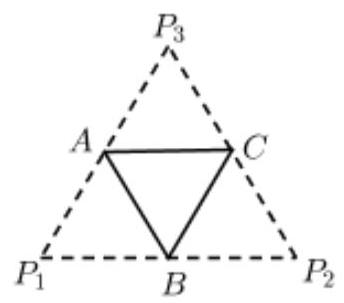
\includegraphics[max width=0.2\textwidth]{images/bo_d6dcisv7aajc739b5agg_65_265_1083_344_303_0.jpg}
\end{center}
\hspace*{3em} 

20. 设常数 \(a \geq  0\) ,函数 \(f\left( x\right)  = \frac{{2}^{x} + a}{{2}^{x} - a}\) .

(1)若 \(a = 4\) ，求函数 \(y = f\left( x\right)\) 的反函数 \(y = {f}^{-1}\left( x\right)\) ；

(2)根据 \(a\) 的不同取值，讨论函数 \(y = f\left( x\right)\) 的奇偶性，并说明理由.

21. 如图,某公司要在 \(A,B\) 两地连线上的定点 \(C\) 处建造广告牌,其中 \(D\) 为顶端, \({AC}\) 长 35 米, \({CB}\) 长 80 米,设点 \(A,B\) 在同一水平面上,从 \(A\) 和 \(B\) 看 \(D\) 的仰角分别为 \(\alpha\) 和 \(\beta\) .

\begin{center}
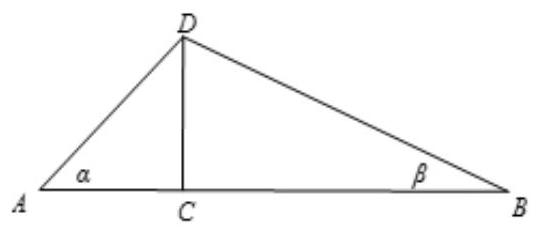
\includegraphics[max width=0.4\textwidth]{images/bo_d6dcisv7aajc739b5agg_66_285_271_536_229_0.jpg}
\end{center}
\hspace*{3em} 

(1)设计中 \({CD}\) 是铅垂方向，若要求 \(\alpha  \geq  {2\beta }\) ，问 \({CD}\) 的长至多为多少(结果精确到 0.01米)？

(2)施工完成后， \({CD}\) 与铅垂方向有偏差，现在实测得 \(\alpha  = {38.12}^{ \circ  }\) ， \(\beta  = {18.45}^{ \circ  }\) ，求 \({CD}\) 的长(结果精确到 0.01 米 )?

22. 在平面直角坐标系 \({xOy}\) 中,对于直线 \(l : {ax} + {by} + c = 0\) 和点 \({P}_{1}\left( {{x}_{1},{y}_{1}}\right) ,{P}_{2}\left( {{x}_{2},{y}_{2}}\right)\) ,记 \(\eta  = \; \left( {a{x}_{1} + b{y}_{1} + c}\right) \left( {a{x}_{2} + b{y}_{2} + c}\right)\) . 若 \(\eta  < 0\) ,则称点 \({P}_{1},{P}_{2}\) 被直线 \(l\) 分隔. 若曲线 \(C\) 与直线 \(l\) 没有公共点,且曲线 \(C\) 上存在点 \({P}_{1},{P}_{2}\) 被直线 \(l\) 分隔,则称直线 \(l\) 为曲线 \(C\) 的一条分隔线.

(1) 求证: 点 \(A\left( {1,2}\right) ,B\left( {-{10}}\right)\) 被直线 \(x + y - 1 = 0\) 分隔;

(2)若直线 \(y = {kx}\) 是曲线 \({x}^{2} - 4{y}^{2} = 1\) 的分隔线，求实数 \(k\) 的取值范围；

23. 已知数列 \(\left\{  {a}_{n}\right\}\) 满足 \(\frac{1}{3}{a}_{n} \leq  {a}_{n + 1} \leq  3{a}_{n},n \in  {N}^{ * },{a}_{1} = 1\) .

(1)若 \({a}_{2} = 2,{a}_{3} = x,{a}_{4} = 9\) ，求 \(x\) 的取值范围；

(2)设 \(\left\{  {a}_{n}\right\}\) 是公比为 \(q\) 的等比数列， \({S}_{n} = {a}_{1} + {a}_{2} + \cdots  + {a}_{n}\) ，若 \(\frac{1}{3}{S}_{n} \leq  {S}_{n + 1} \leq  3{S}_{n}\) ， \(n \in  {N}^{ * }\) ，求 \(q\) 的取值范围;

\section*{2014 春考}

一、填空题(共12小题，每小题 3 分，满分 36 分)

1. 若 \({4}^{x} = {16}\) ,则 \(x =\) \_\_\_\_\_.

2. 计算: \(\mathrm{i}\left( {1 + \mathrm{i}}\right)  =\) \_\_\_\_\_(i为虚数单位).

3.1、1、2、2、5 这五个数的中位数是\_\_\_\_\_.

4. 若函数 \(f\left( x\right)  = {x}^{3} + a\) 为奇函数，则实数 \(a =\) \_\_\_\_\_.

5. 点 \(O\left( {0,0}\right)\) 到直线 \(x + y - 4 = 0\) 的距离是\_\_\_\_\_.

6. 函数 \(y = \frac{1}{x + 1}\) 的反函数为\_\_\_\_\_.

7. 已知等差数列 \(\left\{  {a}_{n}\right\}\) 的首项为 1，公差为 2，则该数列的前 \(n\) 项和 \({S}_{n} =\) \_\_\_\_\_.

8. 已知 \(\cos \alpha  = \frac{1}{3}\) ，则 \(\cos {2\alpha } =\) \_\_\_\_\_.

9. 已知 \(a\) 、 \(b \in  {R}^{ + }\) . 若 \(a + b = 1\) ，则 \({ab}\) 的最大值是\_\_\_\_\_.

10. 在 10 件产品中，有 3 件次品，从中随机取出 5 件，则恰含 1 件次品的概率是\_\_\_\_\_(结果用数值表示).

11. 某货船在 \(O\) 处看灯塔 \(M\) 在北偏东 30 。方向,它以每小时 18 海里的速度向正北方向航行, 经过 40 分钟到达 \(B\) 处,看到灯塔 \(M\) 在北偏东 75 。方向,此时货船到灯塔 \(M\) 的距离为\_\_\_\_\_海里.

12. 已知函数 \(f\left( x\right)  = \frac{x - 2}{x - 1}\) 与 \(g\left( x\right)  = {mx} + 1 - m\) 的图象相交于点 \(A,B\) 两点,若动点 \(P\) 满足 \(\left| {\overrightarrow{PA} + \overrightarrow{PB}}\right|  = 2\) ，则 \(P\) 的轨迹方程是\_\_\_\_\_.

\section*{二、选择题}

13. 两条异面直线所成角的范围是 ( )

A. \(\left( {0,\frac{\pi }{2}}\right)\) B. \(\left( {0,\frac{\pi }{2}}\right\rbrack\) C. \(\left\lbrack  {0,\frac{\pi }{2}}\right)\) D. \(\left\lbrack  {0,\frac{\pi }{2}}\right\rbrack\)

14. 复数 \(2 + \mathrm{i}(\mathrm{i}\) 为虚数单位) 的共轭复数为 ( )

A. \(2 - \mathrm{i}\) B. \(- 2 + \mathrm{i}\) C. \(- 2 - \mathrm{i}\) D. \(1 + 2\mathrm{i}\)

15. 如图是下列函数中某个函数的部分图象, 则该函数是( )

\begin{center}
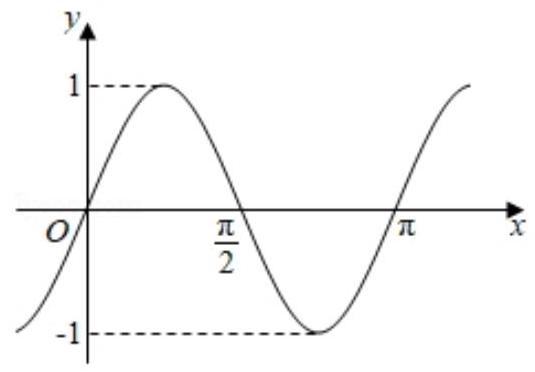
\includegraphics[max width=0.4\textwidth]{images/bo_d6dcisv7aajc739b5agg_69_271_1102_535_372_0.jpg}
\end{center}
\hspace*{3em} 

A. \(y = \sin x\) B. \(y = \sin {2x}\) C. \(y = \cos x\) D. \(y = \cos {2x}\)

16. 在 \({\left( x + 1\right) }^{4}\) 的二项展开式中, \({x}^{2}\) 项的系数为 ( )

A. 6 B. 4 C. 2 D. 1

17. 下列函数中,在 \(R\) 上为增函数的是 ( )

A. \(y = {x}^{2}\) B. \(y = \left| x\right|\) C. \(y = \sin x\) D. \(y = {x}^{3}\)

18. \(\left| \begin{array}{l} \cos \theta \\  \sin \theta  \end{array}\right|  =\) ( )

A. \(\cos {2\theta }\) B. \(\sin {2\theta }\) C. 1 D. -1

19. 设 \({x}_{0}\) 为函数 \(f\left( x\right)  = {2}^{x} + x - 2\) 的零点,则 \({x}_{0} \in\) ( )

A. \(\left( {-2, - 1}\right)\) B. \(\left( {-1,0}\right)\) C. \(\left( {0,1}\right)\) D. \(\left( {1,2}\right)\)

20. 若 \(a,b,c \in  R,a > b\) ,则下列不等式成立的是 ( )

A. \(\frac{1}{a} < \frac{1}{b}\) B. \({a}^{2} > {b}^{2}\) C. \(a\left| c\right|  > b\left| c\right|\) D. \(\frac{a}{{c}^{2} + 1} > \frac{b}{{c}^{2} + 1}\)

21. 若两个球的体积之比为 \(8 : {27}\) ,则它们的表面积之比为 ( )

A. \(2 : 3\) B. \(4 : 9\) C. \(8 : {27}\) D. \(2\sqrt{2} : 3\sqrt{3}\)

22. 如果数列 \(\left\{  {a}_{n}\right\}\) 是一个以 \(q\) 为公比的等比数列, \({b}_{n} =  - 2{a}_{n}\left( {n \in  {N}^{ * }}\right)\) ,那么数列 \(\left\{  {b}_{n}\right\}\) 是 ( )

A. 以 \(q\) 为公比的等比数列 B. 以 \(- q\) 为公比的等比数列

C. 以 \({2q}\) 为公比的等比数列 D. 以 \(- {2q}\) 为公比的等比数列

23. 若点 \(P\) 的坐标为 \(\left( {a,b}\right)\) ,曲线 \(C\) 的方程为 \(F\left( {x,y}\right)  = 0\) ,则 \(F\left( {a,b}\right)  = 0\) 是点 \(P\) 在曲线 \(C\) 上的 ( )

A. 充分非必要条件 B. 必要非充分条件

C. 充要条件 D. 既非充分又非必要条件

24. 如图，在底面半径和高均为 1 的圆锥中， \({AB}\) 、 \({CD}\) 是底面圆 \(O\) 的两条互相垂直的直径， \(E\) 是母线 \({PB}\) 的中点,已知过 \({CD}\) 与 \(E\) 的平面与圆锥侧面的交线是以 \(E\) 为顶点的抛物线的一部分，则该抛物线的焦点到圆锥顶点 \(P\) 的距离为( )

\begin{center}
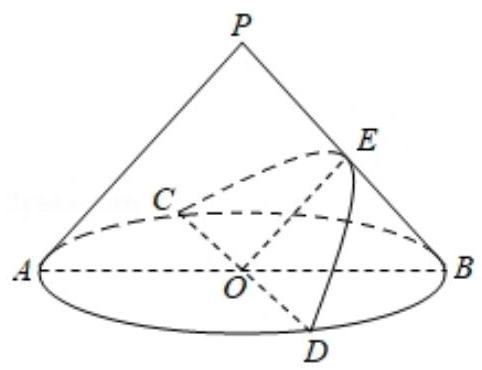
\includegraphics[max width=0.3\textwidth]{images/bo_d6dcisv7aajc739b5agg_71_283_1224_482_370_0.jpg}
\end{center}
\hspace*{3em} 

A. 1

B. \(\frac{\sqrt{3}}{2}\) C. \(\frac{\sqrt{6}}{2}\) D. \(\frac{\sqrt{10}}{4}\)

\section*{三、解答题}

25. 已知不等式 \(\frac{x - 2}{x + 1} < 0\) 的解集为 \(A\) ,函数 \(y = \lg \left( {x - 1}\right)\) 的定义域为集合 \(B\) ,求 \(A \cap  B\) .

26. 已知函数 \(f\left( x\right)  = {x}^{2} - {4x} + a,x \in  \left\lbrack  {-3,3}\right\rbrack\) . 若 \(f\left( 1\right)  = 2\) ,求 \(y = f\left( x\right)\) 的最大值和最小值.

27. 如图，在体积为 \(\frac{1}{3}\) 的三棱锥 \(P - {ABC}\) 中， \({PA}\) 与平面 \({ABC}\) 垂直， \({AP} = {AB} = 1\) ， \(\angle {BAC} \; = \frac{\pi }{2},E\text{ 、 }F\) 分别是 \({PB}\text{ 、 }{AB}\) 的中点. 求异面直线 \({EF}\) 与 \({PC}\) 所成的角的大小 (结果用反三角函数值表示).

\begin{center}
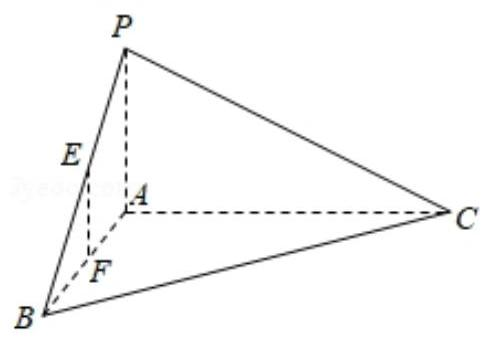
\includegraphics[max width=0.3\textwidth]{images/bo_d6dcisv7aajc739b5agg_72_288_962_486_339_0.jpg}
\end{center}
\hspace*{3em} 

28. 已知椭圆 \(C : \frac{{x}^{2}}{{a}^{2}} + {y}^{2} = 1\left( {a1}\right)\) 的左焦点为 \(F\) ，上顶点为 \(B\) .

(1)若直线 \({FB}\) 的一个方向向量为 \(\left( {1,\frac{\sqrt{3}}{3}}\right)\) ，求实数 \(a\) 的值；

(2) 若 \(a = \sqrt{2}\) ,直线 \(l : y = {kx} - 2\) 与椭圆 \(C\) 相交于 \(M\text{ 、 }N\) 两点,且 \(\overrightarrow{FM}\overrightarrow{FN} = 3\) ,求实数 \(k\) 的值.

29. 已知数列 \(\left\{  {a}_{n}\right\}\) 满足 \({a}_{n} > 0\) ,双曲线 \({C}_{n} : \frac{{x}^{2}}{{a}_{n}} - \frac{{y}^{2}}{{a}_{n + 1}} = 1\left( {n \in  {N}^{ + }}\right)\) .

(1)若 \({a}_{1} = 1,{a}_{2} = 2\) ，双曲线 \({C}_{n}\) 的焦距为 \(2{c}_{n},{c}_{n} = \sqrt{{4n} - 1}\) ，求 \(\left\{  {a}_{n}\right\}\) 的通项公式；

(2)如图，在双曲线 \({C}_{n}\) 的右支上取点 \({P}_{n}\left( {x{p}_{{p}_{n}},n}\right)\) ，过 \({P}_{n}\) 作 \(y\) 轴的垂线，在第一象限内交 \({C}_{n}\) 的渐近线于点 \({Q}_{n}\) ,联结 \(O{P}_{n}\) ,记 \(\bigtriangleup O{P}_{n}{Q}_{n}\) 的面积为 \({S}_{n}\) . 若 \(\mathop{\lim }\limits_{{n \rightarrow  \infty }}{a}_{n} = 2\) ，求 \(\mathop{\lim }\limits_{{n \rightarrow  \infty }}{S}_{n}\) .

30. 已知直角三角形 \({ABC}\) 的两直角边 \({AC}\) 、 \({BC}\) 的边长分别为 \(b\) ， \(a\) ，如图，过 \({AC}\) 边的 \(n\) 等分点 \({A}_{i}\) 作 \({AC}\) 边的垂线 \({d}_{i}\) ，过 \({BC}\) 边的 \(n\) 等分点 \({B}_{i}\) 和顶点 \(A\) 作直线 \({l}_{i}\) ，记 \({d}_{i}\) 与 \({l}_{i}\) 的交点为 \({P}_{i}\) (i \(= 1,2,\cdots \cdots ,n - 1)\) .

是否存在一条圆锥曲线,对任意的正整数 \(n \geq  2\) ,点 \({P}_{i}\left( {\mathrm{i} = 1,2,\cdots \cdots ,n - 1}\right)\) 都在这条曲线上? 说明理由.

\begin{center}
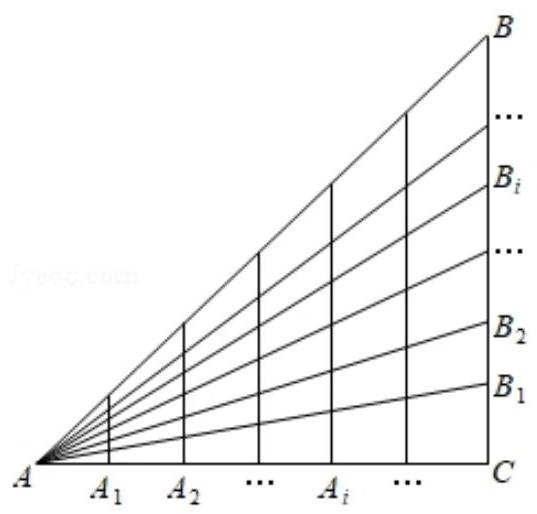
\includegraphics[max width=0.4\textwidth]{images/bo_d6dcisv7aajc739b5agg_73_276_872_537_514_0.jpg}
\end{center}
\hspace*{3em} 

31. 某人造卫星在地球赤道平面绕地球飞行，甲、乙两个监测点分别位于赤道上东经 131。和 147。，在某时刻测得甲监测点到卫星的距离为 1537.45 千米，乙监测点到卫星的距离为 887.64 千米. 假设地球赤道是一个半径为 6378 千米的圆, 求此时卫星所在位置的高度 (结果精确到 0.01 千米) 和经度 (结果精确到 0.01 。).

32. 如果存在非零常数 \(c\) ,对于函数 \(y = f\left( x\right)\) 定义域 \(R\) 上的任意 \(x\) ,都有 \(f\left( {x + c}\right)  > f\left( x\right)\) 成立, 那么称函数为 “ \(Z\) 函数”.

(1)求证:若 \(y = f\left( x\right) \left( {x \in  R}\right)\) 是单调函数，则它是 “ \(Z\) 函数”；

(2)若函数 \(g\left( x\right)  = a{x}^{3} + b{x}^{2}\) 是 “ \(Z\) 函数”，求实数 \(a\) 、 \(b\) 满足的条件.

\section*{2015 秋考}

填空

1. 设全集 \(U = R\) ,若集合 \(A = \{ 1,2,3,4\} ,B = \{ x \mid  2 \leq  x \leq  3\}\) ,则 \(A \cap  {\complement }_{U}B =\) \_\_\_\_\_.

2. 若复数 \(z\) 满足 \({3z} + \bar{z} = 1 + \mathrm{i}\) ，其中 \(\mathrm{i}\) 为虚数单位，则 \(z =\) \_\_\_\_\_.

3. 若线性方程组的增广矩阵为 \(\left( \begin{array}{lll} 2 & 3 & {c}_{1} \\  0 & 1 & {c}_{2} \end{array}\right)\) ,解为 \(\left\{  \begin{array}{l} x = 3 \\  y = 5 \end{array}\right.\) ,则 \({c}_{1} - {c}_{2} =\) \_\_\_\_\_.

4. 若正三棱柱的所有棱长均为 \(a\) ，且其体积为 \({16}\sqrt{3}\) ，则 \(a =\) \_\_\_\_\_.

5. 抛物线 \({y}^{2} = {2px}\left( {p > 0}\right)\) 上的动点 \(Q\) 到焦点的距离的最小值为 1, 则 \(p =\) \_\_\_\_\_.

6. 若圆锥的侧面积与过轴的截面面积之比为 \({2\pi }\) ，则其母线与轴的夹角的大小为\_\_\_\_\_.

7. 方程 \({\log }_{2}\left( {{9}^{x - 1} - 5}\right)  = {\log }_{2}\left( {{3}^{x - 1} - 2}\right)  + 2\) 的解为\_\_\_\_\_.

8. 在报名的 3 名男教师和 6 名女教师中，选取 5 人参加义务献血，要求男、女教师都有，则不同的选取方法的种数为\_\_\_\_\_. (结果用数值表示)

9. 已知点 \(P\) 和 \(Q\) 的横坐标相同， \(P\) 的纵坐标是 \(Q\) 的纵坐标的 2 倍， \(P\) 和 \(Q\) 的轨迹分别为双曲线 \({C}_{1}\) 和 \({C}_{2}\) ，若 \({C}_{1}\) 的渐近线方程为 \(y =  \pm  \sqrt{3}x\) ，则 \({C}_{2}\) 的渐近线方程为\_\_\_\_\_.

10. 设 \({f}^{-1}\left( x\right)\) 为 \(f\left( x\right)  = {2}^{x - 2} + \frac{x}{2},x \in  \left\lbrack  {0,2}\right\rbrack\) 的反函数,则 \(y = f\left( x\right)  + {f}^{-1}\left( x\right)\) 的最大值为\_\_\_\_\_.

11. 在 \({\left( 1 + x + \frac{1}{{x}^{2015}}\right) }^{10}\) 的展开式中， \({x}^{2}\) 项的系数为\_\_\_\_\_. (结果用数值表示)

12. 赌博有陷阱. 某种赌博每局的规则是:赌客现在标有 1,2,3,4,5 的卡片中随机摸取一张, 将卡片上的数字作为其赌金 (单位:元); 随后放回该卡片, 再随机摸取两张, 将两张卡片上数字之差的绝对值的 1.4 倍作为其奖金 (单位:元). 若随机变量 \({\xi }_{1}\) 和 \({\xi }_{2}\) 分别表示赌客在每一局赌博中的赌金与奖金,则 \(E{\xi }_{1} - E{\xi }_{2} =\) \_\_\_\_\_. (元)

13. 已知函数 \(f\left( x\right)  = \sin x\) ,若 \({x}_{1},{x}_{2},\cdots ,{x}_{m}\) 存在满足 \(0 \leq  {x}_{1} < {x}_{2} < \cdots  < {x}_{m} \leq  {6\pi }\) ,且 \(\left| {f\left( {x}_{1}\right)  - f\left( {x}_{2}\right) }\right|  + \left| {f\left( {x}_{2}\right)  - f\left( {x}_{3}\right) }\right|  + \cdots  + \left| {f\left( {x}_{m - 1}\right)  - f\left( {x}_{m}\right) }\right|  = {12}\left( {m \geq  2,m \in  {N}^{ * }}\right)\) ,则 \(m\) 的最小值为\_\_\_\_\_

14. 在锐角 \({\Delta ABC}\) 中, \(\tan A = \frac{1}{2},D\) 为 \({BC}\) 边上的一点, \(\bigtriangleup {ABD}\) 与 \(\bigtriangleup {ACD}\) 面积分别为 2 和 4, 过 \(D\) 作 \({DE} \bot  {AB}\) 于 \(E\) ， \({DF} \bot  {AC}\) 于 \(F\) ，则 \(\overrightarrow{DE} \cdot  \overrightarrow{DF} =\) \_\_\_\_\_.

\begin{center}
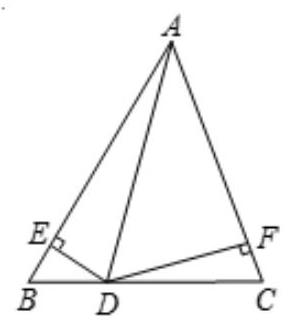
\includegraphics[max width=0.2\textwidth]{images/bo_d6dcisv7aajc739b5agg_76_333_1502_291_325_0.jpg}
\end{center}
\hspace*{3em} 

15. 设 \({z}_{1},{z}_{2} \in  C\) ,则 “ \({z}_{1},{z}_{2}\) 中至少有一个数是虚数” 是 “ \({z}_{1} - {z}_{2}\) 是虚数” 的 ().

A. 充分非必要条件 B. 必要非充分条件

C. 充要条件 D. 既非充分也非必要条件

16. 已知点 \(A\) 的坐标为 \(\left( {4\sqrt{3},1}\right)\) ,将 \({OA}\) 绕坐标原点 \(O\) 逆时针转 \(\frac{\pi }{3}\) 至 \({OB}\) ,则 \(B\) 的纵坐标为 ().

A. \(\frac{3\sqrt{3}}{2}\) B. \(\frac{5\sqrt{3}}{2}\) C. \(\frac{11}{2}\) D. \(\frac{13}{2}\)

17. 记方程 \circled{1} : \({x}^{2} + {a}_{1}x + 1 = 0\) ,方程 \circled{2} : \({x}^{2} + {a}_{2}x + 2 = 0\) ,方程 \circled{3} : \({x}^{2} + {a}_{3}x + 4 = 0\) ,其中 \({a}_{1},{a}_{2},{a}_{3}\) 是正实数. 当 \({a}_{1},{a}_{2},{a}_{3}\) 成等比数列时,下列选项中,能推出方程 \circled{3} 无实根的是 ( ).

A. 方程 \circled{1} 有实根，且 \circled{2} 有实根 B. 方程 \circled{1} 有实根，且 \circled{2} 无实根

C. 方程 \circled{1} 无实根，且 \circled{2} 有实根 D. 方程 \circled{1} 无实根，且 \circled{2} 无实根

18. 设 \({P}_{n}\left( {{x}_{n},{y}_{n}}\right)\) 是直线 \({2x} - y = \frac{n}{n + 1}\left( {n \in  {N}^{ * }}\right)\) 与圆 \({x}^{2} + {y}^{2} = 2\) 在第一象限的交点,则极限 \(\mathop{\lim }\limits_{{n \rightarrow  \infty }}\frac{{y}_{n} - 1}{{x}_{n} - 1} = \left( \right) .\)

A. -1 B. \(- \frac{1}{2}\) C. 1 D. 2

19. 如图，在长方体中 \({ABCD} - {A}_{1}{B}_{1}{C}_{1}{D}_{1}\) ， \(A{A}_{1} = 1\) ， \({AB} = {AD} = 2\) ， \(E\) 、 \(F\) 分别是棱 \({AB}\) 、 \({BC}\) 的中点.

\begin{center}
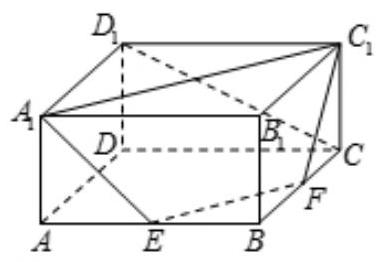
\includegraphics[max width=0.2\textwidth]{images/bo_d6dcisv7aajc739b5agg_78_305_311_381_262_0.jpg}
\end{center}
\hspace*{3em} 

(1)证明 \({A}_{1}\text{ 、 }{C}_{1}\text{ 、 }F\text{ 、 }E\) 四点共面；

(2)求直线 \(C{D}_{1}\) 与平面 \({A}_{1}{C}_{1}{FE}\) 所成角的大小.

20. 如图， \(A\) 、 \(B\) 、 \(C\) 三地有直道相通， \({AB} = 5\) 千米， \({AC} = 3\) 千米， \({BC} = 4\) 千米，现甲、乙两警员同时从 \(A\) 地出发匀速前往 \(B\) 地，经过 \(t\) 小时，他们之间的距离为 \(f\left( t\right)\) (单位:千米). 甲的路线是 \({AB}\) ,速度是 5 千米/小时,乙的路线是 \({ACB}\) ,速度为 8 千米/小时. 乙到达 \(B\) 地后原地等待,设 \(t = {t}_{1}\) 时,乙到达 \(C\) 地.

\begin{center}
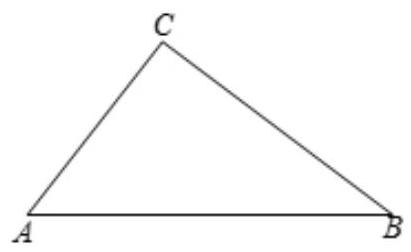
\includegraphics[max width=0.3\textwidth]{images/bo_d6dcisv7aajc739b5agg_78_282_1170_411_252_0.jpg}
\end{center}
\hspace*{3em} 

(1)求 \({t}_{1}\) 与 \(f\left( {t}_{1}\right)\) 的值；

(2)已知警员的对讲机的有效通话距离为 3 千米. 当 \({t}_{1} \leq  t \leq  1\) 时，

21. 已知椭圆 \({x}^{2} + 2{y}^{2} = 1\) ，过原点的两条直线 \({l}_{1}\) 和 \({l}_{2}\) 分别与椭圆交于点 \({AB}\) 和 \({CD}\) ，记得到的平行四边形 \({ACBD}\) 的面积为 \(S\) .

(1)设 \(A\left( {{x}_{1},{y}_{1}}\right) ,C\left( {{x}_{2},{y}_{2}}\right)\) . 用 \({AC}\) 坐标表示点 \(C\) 到直线 \({l}_{1}\) 的距离，并证明 \(S = 2\left| {{x}_{1}{y}_{2} - {x}_{2}{y}_{1}}\right|\) ；

(2) 设 \({l}_{1}\) 与 \({l}_{2}\) 的斜率之积为 \(- \frac{1}{2}\) ,求面积 \(S\) 的值.

22. 已知数列 \(\left\{  {a}_{n}\right\}\) 与 \(\left\{  {b}_{n}\right\}\) 满足 \({a}_{n + 1} - {a}_{n} = 2\left( {{b}_{n + 1} - {b}_{n}}\right) ,n \in  {N}^{ * }\) .

(1) 若 \({b}_{n} = {3n} + 5\) ,且 \({a}_{1} = 1\) ，求 \(\left\{  {a}_{n}\right\}\) 的通项公式；

(2)设 \(\left\{  {a}_{n}\right\}\) 的第 \({n}_{0}\) 项是最大项，即 \({a}_{{n}_{0}} \geq  {a}_{n}\left( {n \in  {N}^{ * }}\right)\) ，求证: \(\left\{  {b}_{n}\right\}\) 的第 \({n}_{0}\) 项是最大项；

23. 对于定义域为 \(R\) 的函数 \(g\left( x\right)\) ,若存在正常数 \(T\) ,使得 \(\cos g\left( x\right)\) 是以 \(T\) 为周期的函数,则称 \(g\left( x\right)\) 为余弦周期函数,且称 \(T\) 为其余弦周期. 已知 \(f\left( x\right)\) 是以 \(T\) 为余弦周期的余弦周期函数,其值域为 \(R\) ,设 \(f\left( x\right)\) 单调递增, \(f\left( 0\right)  = 0,f\left( T\right)  = {4\pi }\) .

(1)验证 \(h\left( x\right)  = x + \sin \frac{x}{3}\) 是以 \({6\pi }\) 为余弦周期的余弦周期函数；

(3)证明: “ \({u}_{0}\) 为方程 \(\cos f\left( x\right)  = 1\) 在 \(\left\lbrack  {0,T}\right\rbrack\) 上的解” 的充要条件是 “ \({u}_{0} + T\) 为方程 \(\cos f\left( x\right)  = 1\) 在 \(\left\lbrack  {T,{2T}}\right\rbrack\) 上的解”,并证明对任意 \(x \in  \left\lbrack  {0,T}\right\rbrack\) 都有 \(f\left( {x + T}\right)  = f\left( x\right)  + f\left( T\right)\) .

\section*{2015 春考}

一、填空题 (每小题 3 分, 满分 36 分)

1. 设全集 \(U = \{ 1,2,3\} ,A = \{ 1,2\}\) ，则 \({\complement }_{U}A =\) \_\_\_\_\_.

2. 计算: \(\frac{1 + i}{i} =\) \_\_\_\_\_(其中 i 为虚数单位).

3. 函数 \(y = \sin \left( {{2x} + \frac{\pi }{4}}\right)\) 的最小正周期是\_\_\_\_\_.

4. 计算: \(\mathop{\lim }\limits_{{n \rightarrow  \infty }}\frac{{n}^{2} - 3}{2{n}^{2} + n} =\) \_\_\_\_\_.

5. 以 \(\left( {2,6}\right)\) 为圆心，1 为半径的圆的标准方程为\_\_\_\_\_.

6. 已知向量 \(\overrightarrow{a} = \left( {1,3}\right) ,\overrightarrow{b} = \left( {m, - 1}\right)\) ，若 \(\overrightarrow{a}\bot \overrightarrow{b}\) ，则 \(m =\) \_\_\_\_\_.

7. 函数 \(y = {x}^{2} - {2x} + 4\) ， \(x \in  \left\lbrack  {0\text{ ， }2}\right\rbrack\) 的值域为\_\_\_\_\_.

8. 若线性方程组的增广矩阵为 \(\left( \begin{array}{l} a \\  0 \end{array}\right)\) ，解为 \(\left\{  \begin{array}{l} x = 2 \\  y = 1 \end{array}\right.\) ，则 \(a + b =\) \_\_\_\_\_.

9. 方程 \(\lg \left( {{2x} + 1}\right)  + \lg x = 1\) 的解集为\_\_\_\_\_.

10. \({\left( x + \frac{1}{{x}^{2}}\right) }^{9}\) 的二项展开式中常数项是\_\_\_\_\_(用数字作答).

11. 用数字 1、2、3、4、5 组成无重复数字的三位数，其中奇数的个数为\_\_\_\_\_. (结果用数值表示)

12. 已知点 \(A\left( {1,0}\right)\) ,直线 \(l : x =  - 1\) ,两个动圆均过点 \(A\) 且与 \(l\) 相切,其圆心分别为 \({C}_{1}\text{ 、 }{C}_{2}\) ,若动点 \(M\) 满足 \(2\overrightarrow{{C}_{2}M} = \overrightarrow{{C}_{2}{C}_{1}} + \overrightarrow{{C}_{2}A}\) ，则 \(M\) 的轨迹方程为\_\_\_\_\_.

\section*{二、选择题 (每小题 3 分, 满分 36 分)}

13. 若 \(a < 0 < b\) ,则下列不等式恒成立的是 ( )

A. \(\frac{1}{a} > \frac{1}{b}\) B. \(- a > b\) C. \({a}^{2} > {b}^{2}\) D. \({a}^{3} < {b}^{3}\)

14. 函数 \(y = {x}^{2}\left( {x \geq  1}\right)\) 的反函数为 ( )

A. \(y = \sqrt{x}\left( {x \geq  1}\right)\) B. \(y = \sqrt{-x}\left( {x \leq   - 1}\right)\)

C. \(y = \sqrt{x}\left( {x \geq  0}\right)\) D. \(y = \sqrt{-x}\left( {x \leq  0}\right)\)

15. 不等式 \(\frac{2 - {3x}}{x - 1} > 0\) 的解集为 ( )

A. \(\left( {-\infty ,\frac{3}{4}}\right)\) B. \(\left( {-\infty ,\frac{2}{3}}\right)\)

C. \(\left( {-\infty ,\frac{2}{3}}\right)  \cup  \left( {1, + \infty }\right)\) D. \(\left( {\frac{2}{3},1}\right)\)

16. 下列函数中,是奇函数且在 \(\left( {0, + \infty }\right)\) 上单调递增的为 ( )

A. \(y = {x}^{2}\) B. \(y = {x}^{\frac{1}{3}}\) C. \(y = {x}^{-1}\) D. \(y = {x}^{-\frac{1}{2}}\)

17. 直线 \({3x} - {4y} - 5 = 0\) 的倾斜角为 ( )

A. \(\arctan \frac{3}{4}\) B. \(\pi  - \arctan \frac{3}{4}\) C. \(\arctan \frac{4}{3}\) D. \(\pi  - \arctan \frac{4}{3}\)

18. 底面半径为 1,母线长为 2 的圆锥的体积为 ( )

A. \({2\pi }\) B. \(\sqrt{3}\pi\) C. \(\frac{2\pi }{3}\) D. \(\frac{\sqrt{3}\pi }{3}\)

19. 以 \(\left( {-3,0}\right)\) 和 \(\left( {3,0}\right)\) 为焦点,长轴长为 8 的椭圆方程为 ( )

A. \(\frac{{x}^{2}}{16} + \frac{{y}^{2}}{25} = 1\) B. \(\frac{{x}^{2}}{16} + \frac{{y}^{2}}{7} = 1\) C. \(\frac{{x}^{2}}{25} + \frac{{y}^{2}}{16} = 1\) D. \(\frac{{x}^{2}}{7} + \frac{{y}^{2}}{16} = 1\)

20. 在复平面上,满足 \(\left| {z - 1}\right|  = \left| {z + \mathrm{i}}\right|\) ( \(\mathrm{i}\) 为虚数单位) 的复数 \(z\) 对应的点的轨迹为 ( )

A. 椭圆 B. 圆 C. 线段 D. 直线

21. 若无穷等差数列 \(\left\{  {a}_{n}\right\}\) 的首项 \({a}_{1} > 0\) ,公差 \(d < 0,\left\{  {a}_{n}\right\}\) 的前 \(n\) 项和为 \({S}_{n}\) ,则 ( )

A. \({S}_{n}\) 单调递减 B. \({S}_{n}\) 单调递增 C. \({S}_{n}\) 有最大值 D. \({S}_{n}\) 有最小值

22. 已知 \(a > 0,b > 0\) ,若 \(a + b = 4\) ,则 ( )

A. \({a}^{2} + {b}^{2}\) 有最小值 B. \(\sqrt{ab}\) 有最小值

C. \(\frac{1}{a} + \frac{1}{b}\) 有最大值 D. \(\frac{1}{\sqrt{a} + \sqrt{b}}\) 有最大值

23. 组合数 \({C}_{n}^{m} + 2{C}_{n}^{m - 1} + {C}_{n}^{m - 2}\left( {n \geq  m \geq  2,m > n \geq  {N}^{ * }}\right.\) 恒等于 ( )

A. \({C}_{n + 2}^{m}\) B. \({C}_{n + 2}^{m + 1}\) C. \({C}_{n + 1}^{m}\) D. \({C}_{n + 1}^{m + 1}\)

24. 设集合 \({P}_{1} = \left\{  {x \mid  {x}^{2} + {ax} + {10}}\right\}  ,{P}_{2} = \left\{  {x \mid  {x}^{2} + {ax} + {20}}\right\}  ,{Q}_{1} = \left\{  {x \mid  {x}^{2} + x + {b0}}\right\}  ,{Q}_{2} = \; \left\{  {x \mid  {x}^{2} + {2x} + {b0}}\right\}\) ,其中 \(a,b \in  R\) ,下列说法正确的是 ( )

A. 对任意 \(a,{P}_{1}\) 是 \({P}_{2}\) 的子集,对任意 \(b,{Q}_{1}\) 不是 \({Q}_{2}\) 的子集

B. 对任意 \(a,{P}_{1}\) 是 \({P}_{2}\) 的子集,存在 \(b\) ,使得 \({Q}_{1}\) 是 \({Q}_{2}\) 的子集

C. 存在 \(a,{P}_{1}\) 不是 \({P}_{2}\) 的子集,对任意 \(b,{Q}_{1}\) 不是 \({Q}_{2}\) 的子集

D. 存在 \(a,{P}_{1}\) 不是 \({P}_{2}\) 的子集,存在 \(b\) ,使得 \({Q}_{1}\) 是 \({Q}_{2}\) 的子集

\section*{三、解答题(共 5 大题，满分 48 分)}

25. 如图,在正四棱柱中 \({ABCD} - {A}_{1}{B}_{1}{C}_{1}{D}_{1},{AB} = 1,{D}_{1}B\) 和平面 \({ABCD}\) 所成的角的大小为 \(\arctan \frac{3\sqrt{2}}{4}\) ,求该四棱柱的表面积.

\begin{center}
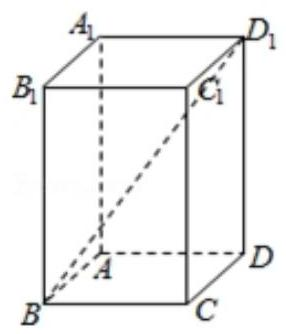
\includegraphics[max width=0.2\textwidth]{images/bo_d6dcisv7aajc739b5agg_84_268_984_286_334_0.jpg}
\end{center}
\hspace*{3em} 

26. 已知 \(a\) 是实数,函数 \(f\left( x\right)  = \frac{{x}^{2} + {ax} + 4}{x}\) 是奇函数,求 \(f\left( x\right)\) 在 \(\left( {0, + \infty }\right)\) 上的最小值及取到最小值时 \(x\) 的值.

27. 某船在海平面 \(A\) 处测得灯塔 \(B\) 在北偏东 30 。方向,与 \(A\) 相距 6.0 海里. 船由 \(A\) 向正北方向航行 8.1 海里达到 \(C\) 处,这时灯塔 \(B\) 与船相距多少海里 (精确到 0.1 海里)? \(B\) 在船的什么方向 (精确到 1 - c)?

28. 已知点 \({F}_{1}\text{ 、 }{F}_{2}\) 依次为双曲线 \(C : \frac{{x}^{2}}{{a}^{2}} - \frac{{y}^{2}}{{b}^{2}} = 1\left( {a,{b0}}\right)\) 的左右焦点, \(\left| {{F}_{1}{F}_{2}}\right|  = 6,{B}_{1}\left( {0, - b}\right)\) , \({B}_{2}\left( {0,b}\right)\) .

(1)若 \(a = \sqrt{5}\) ，以 \(\overrightarrow{d} = \left( {3, - 4}\right)\) 为方向向量的直线 \(l\) 经过 \({B}_{1}\) ，求 \({F}_{2}\) 到 \(l\) 的距离；

29. 已知函数 \(f\left( x\right)  = \left| {{2}^{x - 2} - 2}\right| \left( {x \in  R}\right)\) .

(1)解不等式 \(f\left( x\right)  < 2\) ;

\section*{一、选择题 (本大题满分 9 分) 本大题共有 4 题, 每题有且只有一个正确答案, 考生应在答 题纸的相应编号上, 将代表答案的小方格涂黑, 选对得 3 分, 否则一律得 0 分.}

30. 对于集合 \(A\text{ 、 }B,\) “ \(A \neq  B\) ” 是 “ \(A \cap  B \subsetneqq  A \cup  B\) ” 的 ( )

A. 充分非必要条件 B. 必要非充分条件

C. 充要条件 D. 既非充分也非必要条件

31. 对于任意实数 \(a\text{ 、 }b,{\left( a - b\right) }^{2} \geq  {kab}\) 均成立,则实数 \(k\) 的取值范围是 ( )

A. \(\{  - 4,0\}\) B. \(\left\lbrack  {-4,0}\right\rbrack\)

C. \(( - \infty ,0\rbrack\) D. \(( - \infty , - 4\rbrack  \cup  \lbrack 0, + \infty )\)

32. 已知数列 \(\left\{  {a}_{n}\right\}\) 满足 \({a}_{n} + {a}_{n + 4} = {a}_{n + 1} + {a}_{n + 3}\left( {n \in  {N}^{ * }}\right)\) ,那么必有 ( )

A. \(\left\{  {a}_{n}\right\}\) 是等差数列 B. \(\left\{  {a}_{{2n} - 1}\right\}\) 是等差数列

C. \(\left\{  {a}_{2n}\right\}\) 是等差数列 D. \(\left\{  {a}_{3n}\right\}\) 是等差数列

二、填空题(本大题满分 9 分)本大题共有 3 小题, 考生应在答题纸相应编号的空格内直接填写结果, 每个空格填对得 3 分, 否则一律得 0 分.

33. 关于 \(x\) 的实系数一元二次方程 \({x}^{2} + {px} + 2 = 0\) 的两个虚数根为 \({z}_{1}\text{ 、 }{z}_{2}\) ,若 \({z}_{1}\text{ 、 }{z}_{2}\) 在复平面上对应的点是经过原点的椭圆的两个焦点，则该椭圆的长轴长为\_\_\_\_\_.

34. 已知圆心为 \(O\) ,半径为 1 的圆上有三点 \(A\text{ 、 }B\text{ 、 }C\) ,若 \(7\overrightarrow{OA} + 5\overrightarrow{OB} + 8\overrightarrow{OC} = \overrightarrow{0}\) ,则 \(\left| \overrightarrow{BC}\right|  =\) \_\_\_\_\_.

35. 函数 \(f\left( x\right)\) 与 \(g\left( x\right)\) 的图象拼成如图所示的 “ \(Z\) ” 字形折线段 \({ABOCD}\) ,不含 \(A\left( {0,1}\right)\) , \(B\left( {1,1}\right) ,O\left( {0,0}\right) ,C\left( {-1, - 1}\right) ,D\left( {0, - 1}\right)\) 五个点,若 \(f\left( x\right)\) 的图象关于原点对称的图形即为 \(g\left( x\right)\) 的图象,则其中一个函数的解析式可以为\_\_\_\_\_.

\begin{center}
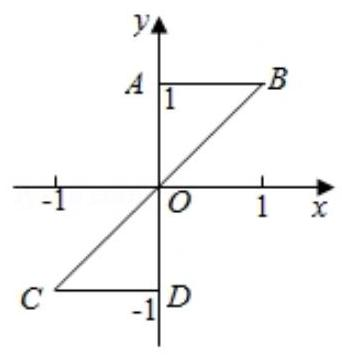
\includegraphics[max width=0.2\textwidth]{images/bo_d6dcisv7aajc739b5agg_86_274_1582_342_356_0.jpg}
\end{center}
\hspace*{3em} 

三、解答题 (本大题满分 12 分) 解答本题必须在答题纸相应编号的规定区域内写出必要的步骤.

36. 对于函数 \(f\left( x\right) \text{ 、 }g\left( x\right)\) ,存在函数 \(h\left( x\right)\) ,使得 \(f\left( x\right)  = g\left( x\right) h\left( x\right)\) ,则称 \(f\left( x\right)\) 是 \(g\left( x\right)\) 的 “ \(h\left( x\right)\) 关联函数”.

(1)已知 \(f\left( x\right)  = \sin x,g\left( x\right)  = \cos x\) ，是否存在定义域为 \(R\) 的函数 \(h\left( x\right)\) ，使得 \(f\left( x\right)\) 是 \(g\left( x\right)\) 的 “ \(h\left( x\right)\) 关联函数”? 若存在,写出 \(h\left( x\right)\) 的解析式; 若不存在,请说明理由;

\section*{2016 秋考}

填空

1. 设 \(x \in  R\) ，则不等式 \(\left| {x - 3}\right|  < 1\) 的解集为\_\_\_\_\_.

2. 设 \(z = \frac{3 + {2i}}{i}\) ，其中 \(\mathrm{i}\) 为虚数单位，则 \(\operatorname{Im}z =\) \_\_\_\_\_.

3. \({l}_{1} : {{2x} + y - 1} = 0,\;{l}_{2} : {{2x} + y + 1} = 0\) ，则 \({l}_{1},{l}_{2}\) 的距离为\_\_\_\_\_.

4. 某次体检, 6 位同学的身高 (单位: 米) 分别为1.72,1.78,1.75,1.80,1.69,1.77,则这组数据的中位数是\_\_\_\_\_(米).

5. 已知点 \(\left( {3,9}\right)\) 在函数 \(f\left( x\right)  = 1 + {a}^{x}\) 的图像上，则 \(f\left( x\right)\) 的反函数 \({f}^{-1}\left( x\right)  =\) \_\_\_\_\_.

6. 如图,在正四棱柱 \({ABCD} - {A}_{1}{B}_{1}{C}_{1}{D}_{1}\) 中,底面 \({ABCD}\) 的边长为 \(3,B{D}_{1}\) 与底面所成角的大小为 \(\arctan \frac{2}{3}\) ，则该正四棱柱的高等于\_\_\_\_\_.

\begin{center}
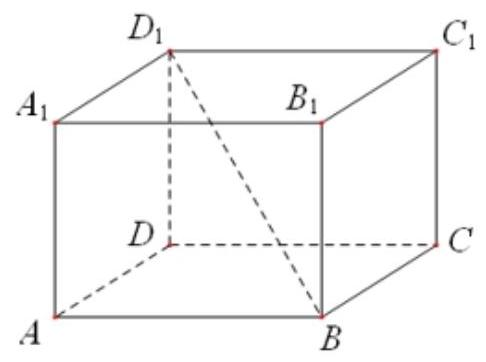
\includegraphics[max width=0.3\textwidth]{images/bo_d6dcisv7aajc739b5agg_88_264_634_486_362_0.jpg}
\end{center}
\hspace*{3em} 

7. 方程 \(3\sin x = 1 + \cos {2x}\) 在区间 \(\left\lbrack  {0,{2\pi }}\right\rbrack\) 上的解为\_\_\_\_\_.

8. 在 \({\left( \sqrt[3]{x} - \frac{2}{x}\right) }^{n}\) 的二项式中，所有项的二项式系数之和为 256，则常数项等于\_\_\_\_\_.

9. 已知 \({ABC}\) 的三边长为3，5，7，则该三角形的外接圆半径等于\_\_\_\_\_.

10. 设 \(a > 0,b > 0\) ,若关于 \(x,y\) 的方程组 \(\left\{  \begin{array}{l} {ax} + y = 1 \\  x + {by} = 1 \end{array}\right.\) 无解,则 \(a + b\) 的取值范围是\_\_\_\_\_.

11. 无穷数列 \(\left\{  {a}_{n}\right\}\) 由 \(k\) 个不同的数组成, \({S}_{n}\) 为 \(\left\{  {a}_{n}\right\}\) 的前 \(n\) 项和,若对任意 \(n \in  {N}^{ * },{S}_{n} \in \; \{ 2,3\}\) ，则 \(k\) 的最大值为\_\_\_\_\_.

12. 在平面直角坐标系中,已知 \(A\left( {1,0}\right) ,\;B\left( {0, - 1}\right) ,\;P\) 是曲线 \(y = \sqrt{1 - {x}^{2}}\) 上一个动点,则 \(\overrightarrow{BP} \cdot  \overrightarrow{BA}\) 的取值范围是\_\_\_\_\_.

13. 设 \(a,b \in  R,c \in  \lbrack 0,{2\pi })\) ,若对任意实数 \(x\) 都有 \(2\sin \left( {{3x} - \frac{\pi }{3}}\right)  = a\sin \left( {{bx} + c}\right)\) ,则满足条件的有序实数 \(\left( {a,b,c}\right)\) 的组数为\_\_\_\_\_.

14. 如图,在平面直角坐标系 \({xOy}\) 中, \(O\) 为正八边形 \({A}_{1}{A}_{2}\cdots {A}_{8}\) 的中心, \({A}_{1}\left( {1,0}\right)\) ,任取不同的两点 \({A}_{i},{A}_{j}\) ，点 \(P\) 满足 \(\overrightarrow{OP} + \overrightarrow{O{A}_{i}} + \overrightarrow{O{A}_{j}} = \overrightarrow{0}\) ，则点 \(P\) 落在第一象限的概率是\_\_\_\_\_.

\begin{center}
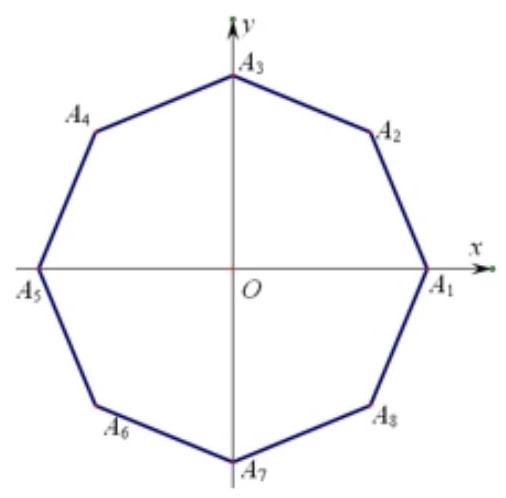
\includegraphics[max width=0.3\textwidth]{images/bo_d6dcisv7aajc739b5agg_90_260_225_506_498_0.jpg}
\end{center}
\hspace*{3em} 

15. 设 \(a \in  R\) ,则 “ \(a > 1\) ” 是 “ \({a}^{2} > 1\) ” 的 ().

A. 充分非必要条件 B. 必要非充分条件

C. 充要条件 D. 既非充分也非必要条件

16. 下列极坐标方程中，对应的曲线为右图的是 ().

\begin{center}
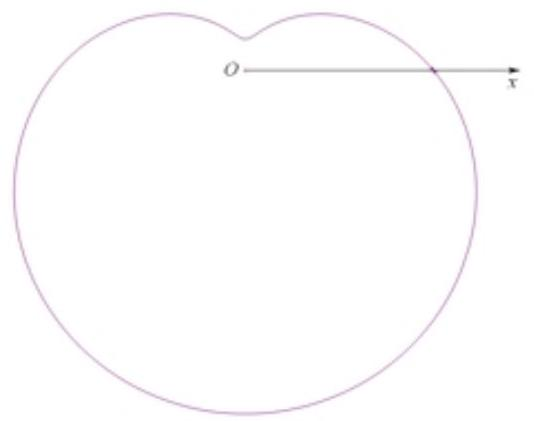
\includegraphics[max width=0.4\textwidth]{images/bo_d6dcisv7aajc739b5agg_90_267_1433_534_421_0.jpg}
\end{center}
\hspace*{3em} 

A. \(\rho  = 6 + 5\cos \theta\) B. \(\rho  = 6 + 5\sin \theta\) C. \(\rho  = 6 - 5\cos \theta\) D. \(\rho  = 6 - 5\sin \theta\)

17. 已知无穷等比数列 \(\left\{  {a}_{n}\right\}\) 的公比为 \(q\) ,前 \(n\) 项和为 \({S}_{n}\) ,且 \(\mathop{\lim }\limits_{{n\infty }}{S}_{n} = S\) ,下列条件中,使得 \(2{S}_{n} \; < S\left( {n \in  {N}^{ * }}\right)\) 恒成立的是 ( ).

A. \({a}_{1} > 0,\;{0.6} < q < {0.7}\) B. \({a}_{1} < 0,\; - {0.7} < q <  - {0.6}\)

C. \({a}_{1} > 0,\;{0.7} < q < {0.8}\) D. \({a}_{1} < 0,\; - {0.8} < q <  - {0.7}\)

18. 设 \(f\left( x\right) ,g\left( x\right) ,h\left( x\right)\) 是定义域为 \(R\) 的三个函数,对于命题:  \circled{1} 若 \(f\left( x\right)  + g\left( x\right) ,f\left( x\right)  + \; h\left( x\right) ,g\left( x\right)  + h\left( x\right)\) 均为增函数,则 \(f\left( x\right) ,g\left( x\right) ,h\left( x\right)\) 中至少有一个为增函数;  \circled{2} 若 \(f\left( x\right) \; + g\left( x\right) ,f\left( x\right)  + h\left( x\right) ,g\left( x\right)  + h\left( x\right)\) 均是以 \(T\) 为周期的函数,则 \(f\left( x\right) ,g\left( x\right) ,h\left( x\right)\) 均是以 \(T\) 为周期的函数,下列判断正确的是 ( ).

A.  \circled{1} 和 \circled{2} 均为真命题 B.  \circled{1} 和 \circled{2} 均为假命题

C.  \circled{1} 为真命题， \circled{2} 为假命题 D.  \circled{1} 为假命题， \circled{2} 为真命题

19. 将边长为 1 的正方形 \(A{A}_{1}{O}_{1}O\) (及其内部) 绕 \(O{O}_{1}\) 旋转一周形成圆柱,如图, \({AC}\) 长为 \(\frac{2}{3}\pi , - {A}_{1}{B}_{1}\) 长为 \(\frac{\pi }{3}\) ,其中 \({B}_{1}\) 与 \(C\) 在平面 \(A{A}_{1}{O}_{1}O\) 的同侧.

\begin{center}
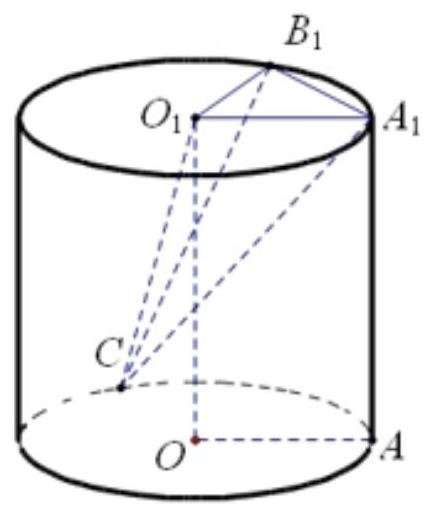
\includegraphics[max width=0.3\textwidth]{images/bo_d6dcisv7aajc739b5agg_91_282_1366_428_507_0.jpg}
\end{center}
\hspace*{3em} 

(1)求三棱锥 \(C - {O}_{1}{A}_{1}{B}_{1}\) 的体积;

20. 有一块正方形菜地 EFGH， \({EH}\) 所在直线是一条小河，收货的蔬菜可送到 \(F\) 点或河边运走. 于是,菜地分为两个区域 \({S}_{1}\) 和 \({S}_{2}\) ,其中 \({S}_{1}\) 中的蔬菜运到河边较近, \({S}_{2}\) 中的蔬菜运到 \(F\) 点较近，而菜地内 \({S}_{1}\) 和 \({S}_{2}\) 的分界线 \(C\) 上的点到河边与到 \(F\) 点的距离相等，现建立平面直角坐标系,其中原点 \(O\) 为 \({EF}\) 的中点,点 \(F\) 的坐标为 \(\left( {1,0}\right)\) ,如图

\begin{center}
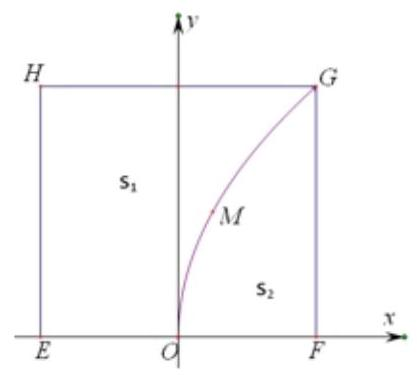
\includegraphics[max width=0.3\textwidth]{images/bo_d6dcisv7aajc739b5agg_92_268_414_417_375_0.jpg}
\end{center}
\hspace*{3em} 

(1)求菜地内的分界线 \(C\) 的方程；

21. 双曲线 \({x}^{2} - \frac{{y}^{2}}{{b}^{2}} = 1\left( {b0}\right)\) 的左、右焦点分别为 \({F}_{1}\text{ 、 }{F}_{2}\) ,直线 \(l\) 过 \({F}_{2}\) 且与双曲线交于 \(A,B\) 两点

(1)若 \(l\) 的倾斜角为 \(\frac{\pi }{2}\) ， \({F}_{1}{AB}\) 是等边三角形，求双曲线的渐近线方程；

22. 已知 \(a \in  R\) ,函数 \(f\left( x\right)  = {\log }_{2}\left( {\frac{1}{x} + a}\right)\)

(1)当 \(a = 5\) 时，解不等式 \(f\left( x\right)  > 0\) ；

(3)设 \(a > 0\) ，若对任意 \(t \in  \left\lbrack  {\frac{1}{2},1}\right\rbrack\) ，函数 \(f\left( x\right)\) 在区间 \(\left\lbrack  {t,t + 1}\right\rbrack\) 上的最大值和最小值的差不超过

1,求 \(a\) 的取值范围.

23. 若无穷数列 \(\left\{  {a}_{n}\right\}\) 满足: 只要 \({a}_{p} = {a}_{q}\left( {p,q \in  {N}^{ * }}\right)\) ,必有 \({a}_{p + 1} = {a}_{q + 1}\) ,则称 \(\left\{  {a}_{n}\right\}\) 具有性质 \(P\) .

(1)若 \(\left\{  {a}_{n}\right\}\) 具有性质 \(P\) . 且 \({a}_{1} = 1,{a}_{2} = 2,{a}_{4} = 3,{a}_{5} = 2,{a}_{6} + {a}_{7} + {a}_{8} = {21}\) ，求 \({a}_{3}\) .

(3)设 \(\left\{  {b}_{n}\right\}\) 是无穷数列，已知 \({a}_{n + 1} = {b}_{n} + \sin {a}_{n}\left( {n \in  {N}^{ * }}\right)\) ，求证:“对任意 \({a}_{1}\) ， \(\left\{  {a}_{n}\right\}\) 都具有性质 \(P\) ”的充要条件为 “ \(\left\{  {b}_{n}\right\}\) 是常数列”.

\section*{2017 秋考}

\section*{填空}

1. 已知集合 \(A = \{ 1,2,3,4\}\) ，集合 \(B = \{ 3,4,5\}\) ，则 \(A \cap  B =\) \_\_\_\_\_

2. 若排列数 \({A}_{6}^{m} = 6 \times  5 \times  4\) ,则 \(m =\) \_\_\_\_\_

3. 不等式 \(\frac{x - 1}{x} > 1\) 的解集为\_\_\_\_\_

4. 已知球的体积为 \({36\pi }\) ，则该球主视图的面积等于\_\_\_\_\_.

5. 已知复数 \(z\) 满足 \(z + \frac{3}{z} = 0\) ，则 \(\left| z\right|  =\) \_\_\_\_\_

6. 设双曲线 \(\frac{{x}^{2}}{9} - \frac{{y}^{2}}{{b}^{2}} = 1\left( {b0}\right)\) 的焦点为 \({F}_{1}\text{ 、 }{F}_{2},P\) 为该双曲线上的一点,若 \(\left| {P{F}_{1}}\right|  = 5\) ,则 \(\left| {P{F}_{2}}\right|  =\) \_\_\_\_\_

7. 如图,以长方体 \({ABCD} - {A}_{1}{B}_{1}{C}_{1}{D}_{1}\) 的顶点 \(D\) 为坐标原点,过 \(D\) 的三条棱所在的直线为坐标轴,建立空间直角坐标系,若 \(\overrightarrow{D{B}_{1}}\) 的坐标为 \(\left( {4,3,2}\right)\) ,则 \(\overrightarrow{A{C}_{1}}\) 的坐标为\_\_\_\_\_

\begin{center}
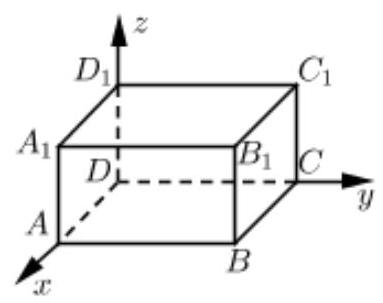
\includegraphics[max width=0.3\textwidth]{images/bo_d6dcisv7aajc739b5agg_94_278_961_383_303_0.jpg}
\end{center}
\hspace*{3em} 

8. 定义在 \(\left( {0, + \infty }\right)\) 上的函数 \(y = f\left( x\right)\) 的反函数为 \(y = {f}^{-1}\left( x\right)\) ,若 \(g\left( x\right)  = \left\{  \begin{array}{ll} {3}^{x} - 1 & x \leq  0 \\  f\left( x\right) & x > 0 \end{array}\right.\) 为奇函数,则 \({f}^{-1}\left( x\right)  = 2\) 的解为\_\_\_\_\_

9. 已知四个函数: \circled{1}  \(y =  - x\) ;  \circled{2}  \(y =  - \frac{1}{x}\) ;  \circled{3}  \(y = {x}^{3}\) ； \circled{4}  \(y = {x}^{\frac{1}{2}}\) . 从中任选 2 个，则事件“所选 2 个函数的图像有且仅有一个公共点” 的概率为\_\_\_\_\_

10. 已知数列 \(\left\{  {a}_{n}\right\}\) 和 \(\left\{  {b}_{n}\right\}\) ,其中 \({a}_{n} = {n}^{2},n \in  {N}^{ * },\left\{  {b}_{n}\right\}\) 的项是互不相等的正整数,若对于任意 \(n \in  {N}^{ * },\;\left\{  {b}_{n}\right\}\) 的第 \({a}_{n}\) 项等于 \(\left\{  {a}_{n}\right\}\) 的第 \({b}_{n}\) 项,则 \(\frac{\lg \left( {{b}_{1}{b}_{4}{b}_{9}{b}_{16}}\right) }{\lg \left( {{b}_{1}{b}_{2}{b}_{3}{b}_{4}}\right) } = \underline{\lim }\)

11. 设 \({\alpha }_{1}\text{ 、 }{\alpha }_{2} \in  R\) ,且 \(\frac{1}{2 + \sin {\alpha }_{1}} + \frac{1}{2 + \sin \left( {2{\alpha }_{2}}\right) } = 2\) ,则 \(\left| {{10\pi } - {\alpha }_{1} - {\alpha }_{2}}\right|\) 的最小值等于\_\_\_\_\_

12. 如图,用 35 个单位正方形拼成一个矩形,点 \({P}_{1}\text{ 、 }{P}_{2}\text{ 、 }{P}_{3}\text{ 、 }{P}_{4}\) 以及四个标记为 “\#” 的点在正方形的顶点处,设集合 \(\Omega  = \left\{  {{P}_{1},{P}_{2},{P}_{3},{P}_{4}}\right\}\) ,点 \(P \in  \Omega\) ,过 \(P\) 作直线 \({l}_{P}\) ,使得不在 \({l}_{P}\) 上的 “\#” 的点分布在 \({l}_{P}\) 的两侧. 用 \({D}_{1}\left( {l}_{P}\right)\) 和 \({D}_{2}\left( {l}_{P}\right)\) 分别表示 \({l}_{P}\) 一侧和另一侧的 “\#” 的点到 \({l}_{P}\) 的距离之和. 若过 \(P\) 的直线 \({l}_{P}\) 中有且只有一条满足 \({D}_{1}\left( {l}_{P}\right)  = {D}_{2}\left( {l}_{P}\right)\) ,则 \(\Omega\) 中所有这样的 \(P\)

为\_\_\_\_\_

\begin{center}
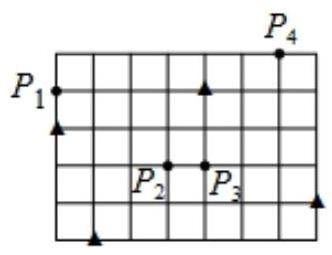
\includegraphics[max width=0.2\textwidth]{images/bo_d6dcisv7aajc739b5agg_95_441_1327_332_255_0.jpg}
\end{center}
\hspace*{3em} 

13. 关于 \(x\text{ 、 }y\) 的二元一次方程组 \(\left\{  \begin{array}{l} x + {5y} = 0 \\  {2x} + {3y} = 4 \end{array}\right.\) 的系数行列式 \(D\) 为( )

A. \(\left| \begin{array}{ll} 0 & 5 \\  4 & 3 \end{array}\right|\) B. \(\left| \begin{array}{ll} 1 & 0 \\  2 & 4 \end{array}\right|\) C. \(\left| \begin{array}{ll} 1 & 5 \\  2 & 3 \end{array}\right|\) D. \(\left| \begin{array}{ll} 6 & 0 \\  5 & 4 \end{array}\right|\)

14. 在数列 \(\left\{  {a}_{n}\right\}\) 中, \({a}_{n} = {\left( -\frac{1}{2}\right) }^{n},n \in  {N}^{ * }\) ,则 \(\mathop{\lim }\limits_{{n \downarrow  \infty }}{a}_{n}\) (   )

A. 等于 \(- \frac{1}{2}\) B. 等于 0 C. 等于 \(\frac{1}{2}\) D. 不存在

15. 已知 \(a\text{ 、 }b\text{ 、 }c\) 为实常数，数列 \(\left\{  {x}_{n}\right\}\) 的通项 \({x}_{n} = a{n}^{2} + {bn} + c\) ， \(n \in  {N}^{ * }\) ，则 “存在 \(k \in  {N}^{ * }\) ， 使得 \({x}_{{100} + k}\text{ 、 }{x}_{{200} + k}\text{ 、 }{x}_{{300} + k}\) 成等差数列” 的一个必要条件是( )

A. \(a \geq  0\) B. \(b \leq  0\) C. \(c = 0\) D. \(a - {2b} + c = 0\)

16. 在平面直角坐标系 \({xOy}\) 中,已知椭圆 \({C}_{1} : \frac{{x}^{2}}{36} + \frac{{y}^{2}}{4} = 1\) 和 \({C}_{2} : {x}^{2} + \frac{{y}^{2}}{9} = 1.P\) 为 \({C}_{1}\) 上的动点, \(Q\) 为 \({C}_{2}\) 上的动点, \(w\) 是 \(\overrightarrow{OP} \cdot  \overrightarrow{OQ}\) 的最大值. 记 \(\Omega  = \{ \left( {P,Q}\right)  \mid  P\) 在 \({C}_{1}\) 上, \(Q\) 在 \({C}_{2}\) 上，且 \(\overrightarrow{OP} \cdot  \overrightarrow{OQ} = w\) ，则 \(\Omega\) 中元素个数为( )

A. 2 个 B. 4 个 C. 8 个 D. 无穷个

17. 如图,直三棱柱 \({ABC} - {A}_{1}{B}_{1}{C}_{1}\) 的底面为直角三角形,两直角边 \({AB}\) 和 \({AC}\) 的长分别为 4 和

2,侧棱 \(A{A}_{1}\) 的长为 5 .

\begin{center}
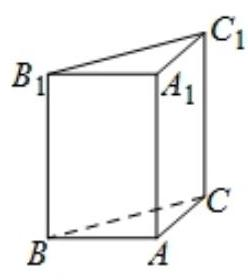
\includegraphics[max width=0.2\textwidth]{images/bo_d6dcisv7aajc739b5agg_96_637_1785_248_280_0.jpg}
\end{center}
\hspace*{3em} 

(1)求三棱柱 \({ABC} - {A}_{1}{B}_{1}{C}_{1}\) 的体积.

(2)设 \(M\) 是 \({BC}\) 中点，求直线 \({A}_{1}M\) 与平面 \({ABC}\) 所成角的大小.

18. 已知函数 \(f\left( x\right)  = {\cos }^{2}x - {\sin }^{2}x + \frac{1}{2},x \in  \left( {0,\pi }\right)\) .

(1) 求 \(f\left( x\right)\) 的单调递增区间.

(2) 设 \({ABC}\) 为锐角三角形,角 \(A\) 所对边 \(a = \sqrt{19}\) ,角 \(B\) 所对边 \(b = 5\) ,若 \(f\left( A\right)  = 0\) ,求 \({ABC}\) 的面积.

19. 根据预测,某地第 \(n\left( {n \in  {N}^{ * }}\right)\) 个月共享单车的投放量和损失量分别为 \({a}_{n}\) 和 \({b}_{n}\) (单位: 辆),其中 \({a}_{n} = \left\{  {\begin{array}{ll} 5{n}^{4} + {15}, & 1 \leq  n \leq  3 \\   - {10n} + {470}, & n \geq  4 \end{array},\;{b}_{n} = n + 5}\right.\) ,第 \(n\) 个月底的共享单车的保有量是前 \(n\) 个月的累计投放量与累计损失量的差.

(1)求该地区第 4 个月底的共享单车的保有量.

(2)已知该地共享单车停放点第 \(n\) 个月底的单车容纳量 \({S}_{n} =  - 4{\left( n - {46}\right) }^{2} + {8800}\) (单位:辆). 设在某月底, 共享单车保有量达到最大, 问该保有量是否超出了此时停放点的单车容纳量?

20. 在平面直角坐标系 \({xOy}\) 中,已知椭圆 \(\Gamma  : \frac{{x}^{2}}{4} + {y}^{2} = 1,A\) 为 \(\Gamma\) 的上顶点， \(P\) 为 \(\Gamma\) 上异于上、下顶点的动点， \(M\) 为 \(x\) 正半轴上的动点.

(1)若 \(P\) 在第一象限，且 \(\left| {OP}\right|  = \sqrt{2}\) ，求 \(P\) 的坐标.

(2)设 \(P\left( {\frac{8}{5},\frac{3}{5}}\right)\) ，若以 \(A\) 、 \(P\) 、 \(M\) 为顶点的三角形是直角三角形，求 \(M\) 的横坐标.

(3) 若 \(\left| {MA}\right|  = \left| {MP}\right|\) ,直线 \({AQ}\) 与 \(\Gamma\) 交于另一点 \(C\) ,且 \(\overrightarrow{AQ} = 2\overrightarrow{AC},\overrightarrow{PQ} = 4\overrightarrow{PM}\) ,求直线 \({AQ}\) 的方程.

21. 设定义在 \(R\) 上的函数 \(f\left( x\right)\) 满足: 对于任意的 \({x}_{1}\text{ 、 }{x}_{2} \in  R\) ,当 \({x}_{1} < {x}_{2}\) 时,都有 \(f\left( {x}_{1}\right)  \leq \; f\left( {x}_{2}\right)\) .

(1) 若 \(f\left( x\right)  = a{x}^{3} + 1\) ，求 \(a\) 的取值范围.

(2)若 \(f\left( x\right)\) 为周期函数，证明: \(f\left( x\right)\) 是常值函数.

(3)设 \(f\left( x\right)\) 恒大于零， \(g\left( x\right)\) 是定义在 \(R\) 上、恒大于零的周期函数， \(M\) 是 \(g\left( x\right)\) 的最大值. 函数 \(h\left( x\right)  = f\left( x\right) g\left( x\right)\) . 证明: “ \(h\left( x\right)\) 是周期函数” 的充要条件是 “ \(f\left( x\right)\) 是常值函数”.

\section*{2017春考}

一. 填空题 (本大题共 12 题,满分 48 分,第 \(1 \sim  6\) 题每题 4 分,第 \(7 \sim  {12}\) 题每题 5 分)

1. 设集合 \(A = \{ 1,2,3\}\) ，集合 \(B = \{ 3,4\}\) ，则 \(A \cup  B =\) \_\_\_\_\_.

2. 不等式 \(\left| {x - 1}\right|  < 3\) 的解集为\_\_\_\_\_.

3. 若复数 \(z\) 满足 \(2\bar{z} - 1 = 3 + 6\mathrm{i}\) ( \(\mathrm{i}\) 是虚数单位),则 \(z =\) \_\_\_\_\_.

4. 若 \(\cos \alpha  = \frac{1}{3}\) ,则 \(\sin \left( {\alpha  - \frac{\pi }{2}}\right)  =\) \_\_\_\_\_.

5. 若关于 \(x\text{ 、 }y\) 的方程组 \(\left\{  \begin{array}{l} x + {2y} = 4 \\  {3x} + {ay} = 6 \end{array}\right.\) 无解,则实数 \(a =\) \_\_\_\_\_.

6. 若等差数列 \(\left\{  {a}_{n}\right\}\) 的前 5 项的和为 25 ,则 \({a}_{1} + {a}_{5} =\) \_\_\_\_\_.

7. 若 \(P\text{ 、 }Q\) 是圆 \({x}^{2} + {y}^{2} - {2x} + {4y} + 4 = 0\) 上的动点,则 \(\left| {PQ}\right|\) 的最大值为\_\_\_\_\_.

8. 已知数列 \(\left\{  {a}_{n}\right\}\) 的通项公式为 \({a}_{n} = {3}^{n}\) ,则 \(\mathop{\lim }\limits_{{n \rightarrow  \infty }}\frac{{a}_{1} + {a}_{2} + {a}_{3} + \cdots  + {a}_{n}}{{a}_{n}} =\) \_\_\_\_\_.

9. 若 \({\left( x + \frac{2}{x}\right) }^{n}\) 的二项展开式的各项系数之和为 729 ，则该展开式中常数项的值为\_\_\_\_\_.

10. 设椭圆 \(\frac{{x}^{2}}{2} + {y}^{2} = 1\) 的左、右焦点分别为 \({F}_{1}\text{ 、 }{F}_{2}\) ,点 \(P\) 在该椭圆上,则使得 \(\bigtriangleup {F}_{1}{F}_{2}P\) 是等腰三角形的点 \(P\) 的个数是\_\_\_\_\_.

11. 设 \({a}_{1}\text{ 、 }{a}_{2}\text{ 、 }\cdots \text{ 、 }{a}_{6}\) 为 \(1\text{ 、 }2\text{ 、 }3\text{ 、 }4\text{ 、 }5\text{ 、 }6\) 的一个排列,则满足 \(\left| {{a}_{1} - {a}_{2}}\right|  + \left| {{a}_{3} - {a}_{4}}\right|  +  \mid  {a}_{5} - \; {a}_{6} \mid   = 3\) 的不同排列的个数为\_\_\_\_\_.

12. 设 \(a\text{ 、 }b \in  R\) ,若函数 \(f\left( x\right)  = x + \frac{a}{x} + b\) 在区间 \(\left( {1,2}\right)\) 上有两个不同的零点,则 \(f\left( 1\right)\) 的取值范围为\_\_\_\_\_.

\section*{二. 选择题 (本大题共 4 题, 每题 5 分, 共 20 分)}

13. 函数 \(f\left( x\right)  = {\left( x - 1\right) }^{2}\) 的单调递增区间是 ( )

A. \(\lbrack 0, + \infty )\) B. \(\lbrack 1, + \infty )\) C. \(( - \infty ,0\rbrack\) D. \(( - \infty ,1\rbrack\)

14. 设 \(a \in  R,\) “ \(a > 0\) ” 是 “ \(\frac{1}{a} > 0\) ” 的 ( ) 条件.

A. 充分非必要 B. 必要非充分 C. 充要 D. 既非充分也非必要

15. 过正方体中心的平面截正方体所得的截面中, 不可能的图形是 ( )

A. 三角形 B. 长方形

C. 对角线不相等的菱形 D. 六边形

16. 如图所示,正八边形 \({A}_{1}{A}_{2}{A}_{3}{A}_{4}{A}_{5}{A}_{6}{A}_{7}{A}_{8}\) 的边长为 2,若 \(P\) 为该正八边形边上的动点,则 \(\overrightarrow{{A}_{1}{A}_{3}}\overrightarrow{{A}_{1}P}\) 的取值范围为( )

\begin{center}
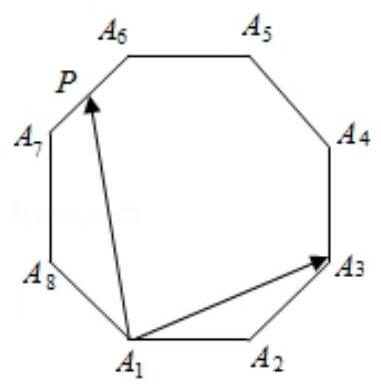
\includegraphics[max width=0.2\textwidth]{images/bo_d6dcisv7aajc739b5agg_101_264_331_381_387_0.jpg}
\end{center}
\hspace*{3em} 

A. \(\left\lbrack  {0,8 + 6\sqrt{2}}\right\rbrack\) B. \(\left\lbrack  {-2\sqrt{2},8 + 6\sqrt{2}}\right\rbrack\)

C. \(\left\lbrack  {-8 - 6\sqrt{2},2\sqrt{2}}\right\rbrack\) D. \(\left\lbrack  {-8 - 6\sqrt{2},8 + 6\sqrt{2}}\right\rbrack\)

三. 解答题 (本大题共 5 题, 共 \({14} + {14} + {14} + {16} + {18} = {76}\) 分)

17. 如图,长方体 \({ABCD} - {A}_{1}{B}_{1}{C}_{1}{D}_{1}\) 中, \({AB} = {BC} = 2,A{A}_{1} = 3\) .

\begin{center}
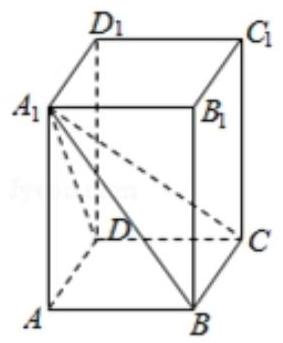
\includegraphics[max width=0.2\textwidth]{images/bo_d6dcisv7aajc739b5agg_101_270_1243_283_343_0.jpg}
\end{center}
\hspace*{3em} 

(1)求四棱锥 \({A}_{1} - {ABCD}\) 的体积；

(2)求异面直线 \({A}_{1}C\) 与 \(D{D}_{1}\) 所成角的大小.

18. 设 \(a \in  R\) ,函数 \(f\left( x\right)  = \frac{{2}^{x} + a}{{2}^{x} + 1}\) .

(1)求 \(a\) 的值，使得 \(f\left( x\right)\) 为奇函数；

(2) 若 \(f\left( x\right)  < \frac{a + 2}{2}\) 对任意 \(x \in  R\) 成立,求 \(a\) 的取值范围.

19. 某景区欲建造两条圆形观景步道 \({M}_{1}\) 、 \({M}_{2}\) (宽度忽略不计),如图所示,已知 \({AB} \bot  {AC}\) ， \({AB} = {AC} = {AD} = {60}\) (单位:米)，要求圆 \({M}_{1}\) 与 \({AB}\) 、 \({AD}\) 分别相切于点 \(B\) 、 \(D\) ，圆 \({M}_{2}\) 与 \({AC}\text{ 、 }{AD}\) 分别相切于点 \(C\text{ 、 }D\) ;

\begin{center}
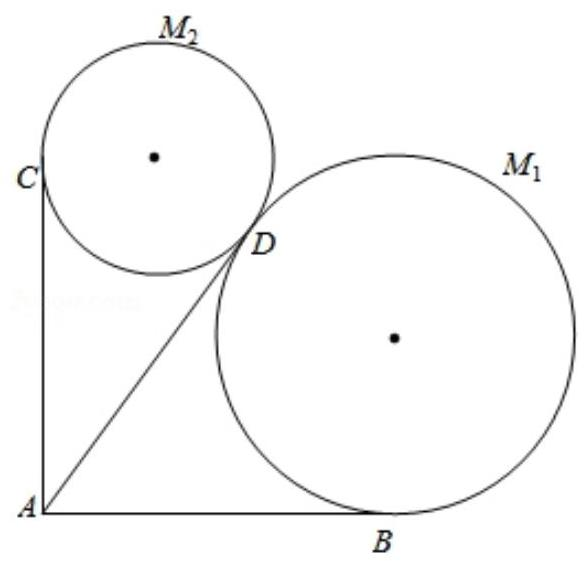
\includegraphics[max width=0.4\textwidth]{images/bo_d6dcisv7aajc739b5agg_102_278_711_585_561_0.jpg}
\end{center}
\hspace*{3em} 

(1)若 \(\angle {BAD} = {60}\) ，求圆 \({M}_{1}\text{ 、 }{M}_{2}\) 的半径 (结果精确到 0.1 米)

(2)若观景步道 \({M}_{1}\) 与 \({M}_{2}\) 的造价分别为每米 0.8 千元与每米 0.9 千元，如何设计圆 \({M}_{1}\text{ 、 }{M}_{2}\) 的大小, 使总造价最低? 最低总造价是多少? (结果精确到 0.1 千元)

20. 已知双曲线 \(\Gamma  : {x}^{2} - \frac{{y}^{2}}{{b}^{2}} = 1\left( {b0}\right)\) ,直线 \(l : y = {kx} + m\left( {\mathrm{\;{km}} \neq  0}\right) ,l\) 与 \(\Gamma\) 交于 \(P\text{ 、 }Q\) 两点, \({P}^{\prime }\) 为 \(P\) 关于 \(y\) 轴的对称点,直线 \({P}^{\prime }Q\) 与 \(y\) 轴交于点 \(N\left( {0,n}\right)\) ;

(1)若点 \(\left( {2,0}\right)\) 是 \(\Gamma\) 的一个焦点，求 \(\Gamma\) 的渐近线方程；

(2)若 \(b = 1\) ，点 \(P\) 的坐标为 \(\left( {-1,0}\right)\) ，且 \(\overrightarrow{N{P}^{\prime }} = \frac{3}{2}\overrightarrow{{P}^{\prime }Q}\) ，求 \(k\) 的值；

(3)若 \(m = 2\) ，求 \(n\) 关于 \(b\) 的表达式.

21. 已知函数 \(f\left( x\right)  = {\log }_{2}\frac{1 + x}{1 - x}\) ;

(1)解方程 \(f\left( x\right)  = 1\) ；

(2)设 \(x \in  \left( {-1,1}\right)\) ， \(a \in  \left( {1, + \infty }\right)\) ，证明: \(\frac{{ax} - 1}{a - x} \in  \left( {-1,1}\right)\) ，且 \(f\left( \frac{{ax} - 1}{a - x}\right)  - f\left( x\right)  =  - f\left( \frac{1}{a}\right)\) ；

(3)设数列 \(\left\{  {x}_{n}\right\}\) 中， \({x}_{1} \in  \left( {-1,1}\right)\) ， \({x}_{n + 1} = {\left( -1\right) }^{n + 1}\frac{3{x}_{n} - 1}{3 - {x}_{n}}\) ， \(n \in  {N}^{ * }\) ，求 \({x}_{1}\) 的取值范围，使得 \({x}_{3} \; \geq  {x}_{n}\) 对任意 \(n \in  {N}^{ * }\) 成立.

\section*{2018 秋考}

选择题

一、填空题

1. 行列式 \(\left| \begin{array}{ll} 4 & 1 \\  2 & 5 \end{array}\right|\) 的值为\_\_\_\_\_.

2. 双曲线 \(\frac{{x}^{2}}{4} - {y}^{2} = 1\) 的渐近线方程为\_\_\_\_\_.

3. 在 \({\left( 1 + x\right) }^{7}\) 的二项展开式中， \({x}^{2}\) 项的系数为\_\_\_\_\_. (结果用数值表示)

4. 设常数 \(a \in  R\) ,函数 \(f\left( x\right)  = {\log }_{2}\left( {x + a}\right)\) ,若 \(f\left( x\right)\) 的反函数的图像经过点 \(\left( {3,1}\right)\) ,则 \(a =\) \_\_\_\_\_.

5. 已知复数 \(z\) 满足 \(\left( {1 + \mathrm{i}}\right) z = 1 - 7\mathrm{i}\) ( \(\mathrm{i}\) 是虚数单位),则 \(\left| z\right|  =\) \_\_\_\_\_.

6. 记等差数列 \(\left\{  {a}_{n}\right\}\) 的前几项和为 \({S}_{n}\) ,若 \({a}_{3} = 0,{a}_{6} + {a}_{7} = {14}\) ,则 \({S}_{7} =\) \_\_\_\_\_.

7. 已知 \(\alpha  \in  \left\{  {-2, - 1, - \frac{1}{2},\frac{1}{2},1,2,3}\right\}\) ,若幂函数 \(f\left( x\right)  = {x}^{\alpha }\) 为奇函数,且在 \(\left( {0, + \infty }\right)\) 上递减, 则 \(\alpha  =\) \_\_\_\_\_.

8. 在平面直角坐标系中,已知点 \(A\left( {-1,0}\right) ,B\left( {2,0}\right) ,E,F\) 是 \(y\) 轴上的两个动点,且 \(\left| \overrightarrow{EF}\right|  =\) 2，则 \(\overrightarrow{AE} \cdot  \overrightarrow{BF}\) 的最小值为\_\_\_\_\_.

9. 有编号互不相同的五个砝码, 其中 5 克、 3 克、 1 克砝码各一个, 2 克砝码两个, 从中随机选取三个，则这三个砝码的总质量为 9 克的概率是\_\_\_\_\_. (结果用最简分数表示)

10. 设等比数列 \(\left\{  {a}_{n}\right\}\) 的通项公式为 \({a}_{n} = {q}^{n + 1}\left( {n \in  {N}^{ * }}\right)\) ,前 \(n\) 项和为 \({S}_{n}\) . 若 \(\mathop{\lim }\limits_{{n \rightarrow  \infty }}\frac{{S}_{n}}{{a}_{n + 1}} = \frac{1}{2}\) ,则 \(q \; =\) \_\_\_\_\_.

11. 已知常数 \(a > 0\) ,函数 \(f\left( x\right)  = \frac{{2}^{x}}{\left( {2}^{x} + ax\right) }\) 的图像经过点 \(P\left( {p,\frac{6}{5}}\right) \text{ 、 }Q\left( {q, - \frac{1}{5}}\right)\) ,若 \({2}^{p + q} = \; {36pq}\) ,则 \(a =\) \_\_\_\_\_.

12. 已知实数 \({x}_{1}\text{ 、 }{x}_{2}\text{ 、 }{y}_{1}\text{ 、 }{y}_{2}\) 满足: \({x}_{1}^{2} + {y}_{1}^{2} = 1,{x}_{2}^{2} + {y}_{2}^{2} = 1,{x}_{1}{x}_{2} + {y}_{1}{y}_{2} = \frac{1}{2}\) ,则 \(\frac{\left| {x}_{1} + {y}_{1} - 1\right| }{\sqrt{2}} \; + \frac{\left| {x}_{2} + {y}_{2} - 1\right| }{\sqrt{2}}\) 的最大值为\_\_\_\_\_.

\section*{二、选择题}

13. 设 \(P\) 是椭圆 \(\frac{{x}^{2}}{5} + \frac{{y}^{2}}{3} = 1\) 上的动点,则 \(P\) 到该椭圆的两个焦点的距离之和为 ( )

A. \(2\sqrt{2}\) B. \(2\sqrt{3}\) C. \(2\sqrt{5}\) D. \(4\sqrt{2}\)

14. 已知 \(a \in  R\) ,则 “ \(a > 1\) ” 是 “ \(\frac{1}{a} < 1\) ” 的 ( )

A. 充分非必要条件 B. 必要非充分条件

C. 充要条件 D. 既非充分又非必要条件

15.《九章算术》中，称底面为矩形而有一侧棱垂直于底面的四棱锥为阳马. 设 \(A{A}_{1}\) 是正六棱柱的一条侧棱,如图,若阳马以该正六棱柱的顶点为顶点,以 \(A{A}_{1}\) 为底面矩形的一边,则这

样的阳马的个数是 ()

\begin{center}
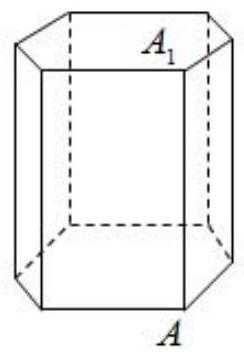
\includegraphics[max width=0.2\textwidth]{images/bo_d6dcisv7aajc739b5agg_106_619_1586_244_359_0.jpg}
\end{center}
\hspace*{3em} 

A. 4 B. 8 C. 12 D. 16

16. 设 \(D\) 是含数 1 的有限实数集, \(f\left( x\right)\) 是定义在 \(D\) 上的函数,若 \(f\left( x\right)\) 的图像绕原点逆时针旋转 \(\frac{\pi }{6}\) 后与原图像重合,则在以下各项中, \(f\left( 1\right)\) 的可能取值只能是 ( )

A. \(\sqrt{3}\) B. \(\frac{\sqrt{3}}{2}\) C. \(\frac{\sqrt{3}}{3}\) D. 0

\section*{三、解答题}

17. 已知圆锥的顶点为 \(P\) ,底面圆心为 \(O\) ,半径为 2 .

(1)设圆锥的母线长为 4，求圆锥的体积；

(2)设 \({PO} = 4,{OA}\) ， \({OB}\) 是底面半径，且 \(\angle {AOB} = {90}^{ \circ  }\) ， \(M\) 为线段 \({AB}\) 的中点，如图，求异面直线 \({PM}\) 与 \({OB}\) 所成的角的大小.

18. 设常数 \(a \in  R\) ,函数 \(f\left( x\right)  = a\sin {2x} + 2{\cos }^{2}x\) .

(1)若 \(f\left( x\right)\) 为偶函数，求 \(a\) 的值；

(2)若 \(f\left( \frac{\pi }{4}\right)  = \sqrt{3} + 1\) ，求方程 \(f\left( x\right)  = 1 - \sqrt{2}\) 在区间 \(\left\lbrack  {-\pi ,\pi }\right\rbrack\) 上的解.

19. 某群体的人均通勤时间, 是指单日内该群体中成员从居住地到工作地的平均用时, 某地上班族 \(S\) 中的成员仅以自驾或公交方式通勤，分析显示:当 \(S\) 中 \(x\% \left( {0 < x < {100}}\right)\) 的成员自驾时,自驾群体的人均通勤时间为 \(f\left( x\right)  = \left\{  \begin{array}{l} {30} \\  {2x} + \frac{1800}{x} - {90} \end{array}\right.\) (单位: 分钟),而公交群体的人均通勤时间不受 \(x\) 影响,恒为 40 分钟,试根据上述分析结果回答下列问题:

(1)当 \(x\) 在什么范围内时，公交群体的人均通勤时间少于自驾群体的人均通勤时间；

(2)求该地上班族 \(S\) 的人均通勤时间 \(g\left( x\right)\) 的表达式；讨论 \(g\left( x\right)\) 的单调性，并说明其实际意义.

20. 设常数 \(t > 2\) ,在平面直角坐标系 \({xOy}\) 中,已知点 \(F\left( {2,0}\right)\) ,直线 \(l : x = t\) ,曲线 \(\tau  : {y}^{2} = \; {8x}\left( {0 \leq  x \leq  t,y \geq  0}\right)\) ， \(l\) 与 \(x\) 轴交于点 \(A\) ，与 \(\tau\) 交于点 \(B\) ， \(P\) 、 \(Q\) 分别是曲线 \(\tau\) 与线段 \({AB}\) 上的动点.

(1) 用 \(t\) 为表示点 \(B\) 到点 \(F\) 的距离;

(2)设 \(t = 3\) ， \(\left| {FQ}\right|  = 2\) ，线段 \({OQ}\) 的中点在直线 \({FP}\) 上，求 \({AQP}\) 的面积；

(3) 设 \(t = 8\) ，是否存在以 \({FP}\) 、 \({FQ}\) 为邻边的矩形 \({FPEQ}\) ，使得点 \(E\) 在 \(\tau\) 上? 若存在，求点 \(P\) 的坐标; 若不存在, 说明理由.

21. 给定无穷数列 \(\left\{  {a}_{n}\right\}\) ，若无穷数列 \(\left\{  {b}_{n}\right\}\) 满足:对任意 \(n \in  {N}^{ * }\) ，都有 \(\left| {{b}_{n} - {a}_{n}}\right|  \leq  1\) ，则称 \(\left\{  {b}_{n}\right\}\) 与 \(\left\{  {a}_{n}\right\}\) “接近”.

(1)设 \(\left\{  {a}_{n}\right\}\) 是首项为 1，公比为 \(\frac{1}{2}\) 的等比数列， \({b}_{n} = {a}_{n + 1} + 1\) ， \(n \in  {N}^{ * }\) ，判断数列 \(\left\{  {b}_{n}\right\}\) 是否与 \(\left\{  {a}_{n}\right\}\) 接近,并说明理由

(2)设数列 \(\left\{  {a}_{n}\right\}\) 的前四项为: \({a}_{1} = 1,{a}_{2} = 2,{a}_{ = }4,{a}_{4} = 8\) ， \(\left\{  {b}_{n}\right\}\) 是一个与 \(\left\{  {a}_{n}\right\}\) 接近的数，记集合 \(M = \left\{  {x \mid   = {b}_{i},\mathrm{i} = 1,2,3,4}\right\}\) ,求 \(M\) 中元素的个数 \(m\)

(3)已知 \(\left\{  {a}_{n}\right\}\) 是公差为 \(d\) 的等差数列，若存在数列 \(\left\{  {b}_{n}\right\}\) 满足: \(\left\{  {b}_{n}\right\}\) 与 \(\left\{  {a}_{n}\right\}\) 接近，且在 \({b}_{2} - {b}_{1}\) ， \({b}_{3} - {b}_{2},\cdots ,{b}_{201} - {b}_{200}\) 中至少有 100 个为正数,求 \(d\) 的取值范围

\section*{2018 秋考}

选择题

一、填空题

1. 行列式 \(\left| \begin{array}{ll} 4 & 1 \\  2 & 5 \end{array}\right|\) 的值为\_\_\_\_\_.

2. 双曲线 \(\frac{{x}^{2}}{4} - {y}^{2} = 1\) 的渐近线方程为\_\_\_\_\_.

3. 在 \({\left( 1 + x\right) }^{7}\) 的二项展开式中， \({x}^{2}\) 项的系数为\_\_\_\_\_. (结果用数值表示)

4. 设常数 \(a \in  R\) ,函数 \(f\left( x\right)  = {\log }_{2}\left( {x + a}\right)\) ,若 \(f\left( x\right)\) 的反函数的图像经过点 \(\left( {3,1}\right)\) ,则 \(a =\) \_\_\_\_\_.

5. 已知复数 \(z\) 满足 \(\left( {1 + \mathrm{i}}\right) z = 1 - 7\mathrm{i}\) ( \(\mathrm{i}\) 是虚数单位),则 \(\left| z\right|  =\) \_\_\_\_\_.

6. 记等差数列 \(\left\{  {a}_{n}\right\}\) 的前几项和为 \({S}_{n}\) ,若 \({a}_{3} = 0,{a}_{6} + {a}_{7} = {14}\) ,则 \({S}_{7} =\) \_\_\_\_\_.

7. 已知 \(\alpha  \in  \left\{  {-2, - 1, - \frac{1}{2},\frac{1}{2},1,2,3}\right\}\) ,若幂函数 \(f\left( x\right)  = {x}^{\alpha }\) 为奇函数,且在 \(\left( {0, + \infty }\right)\) 上递减, 则 \(\alpha  =\) \_\_\_\_\_.

8. 在平面直角坐标系中,已知点 \(A\left( {-1,0}\right) ,B\left( {2,0}\right) ,E,F\) 是 \(y\) 轴上的两个动点,且 \(\left| \overrightarrow{EF}\right|  =\) 2，则 \(\overrightarrow{AE} \cdot  \overrightarrow{BF}\) 的最小值为\_\_\_\_\_.

9. 有编号互不相同的五个砝码, 其中 5 克、 3 克、 1 克砝码各一个, 2 克砝码两个, 从中随机选取三个，则这三个砝码的总质量为 9 克的概率是\_\_\_\_\_. (结果用最简分数表示)

10. 设等比数列 \(\left\{  {a}_{n}\right\}\) 的通项公式为 \({a}_{n} = {q}^{n + 1}\left( {n \in  {N}^{ * }}\right)\) ,前 \(n\) 项和为 \({S}_{n}\) . 若 \(\mathop{\lim }\limits_{{n \rightarrow  \infty }}\frac{{S}_{n}}{{a}_{n + 1}} = \frac{1}{2}\) ,则 \(q \; =\) \_\_\_\_\_.

11. 已知常数 \(a > 0\) ,函数 \(f\left( x\right)  = \frac{{2}^{x}}{\left( {2}^{x} + ax\right) }\) 的图像经过点 \(P\left( {p,\frac{6}{5}}\right) \text{ 、 }Q\left( {q, - \frac{1}{5}}\right)\) ,若 \({2}^{p + q} = \; {36pq}\) ,则 \(a =\) \_\_\_\_\_.

12. 已知实数 \({x}_{1}\text{ 、 }{x}_{2}\text{ 、 }{y}_{1}\text{ 、 }{y}_{2}\) 满足: \({x}_{1}^{2} + {y}_{1}^{2} = 1,{x}_{2}^{2} + {y}_{2}^{2} = 1,{x}_{1}{x}_{2} + {y}_{1}{y}_{2} = \frac{1}{2}\) ,则 \(\frac{\left| {x}_{1} + {y}_{1} - 1\right| }{\sqrt{2}} \; + \frac{\left| {x}_{2} + {y}_{2} - 1\right| }{\sqrt{2}}\) 的最大值为\_\_\_\_\_.

\section*{二、选择题}

13. 设 \(P\) 是椭圆 \(\frac{{x}^{2}}{5} + \frac{{y}^{2}}{3} = 1\) 上的动点，则 \(P\) 到该椭圆的两个焦点的距离之和为( )

A. \(2\sqrt{2}\) B. \(2\sqrt{3}\) C. \(2\sqrt{5}\) D. \(4\sqrt{2}\)

14. 已知 \(a \in  R\) ,则 “ \(a > 1\) ” 是 “ \(\frac{1}{a} < 1\) ” 的 ( )

A. 充分非必要条件 B. 必要非充分条件

C. 充要条件 D. 既非充分又非必要条件

15.《九章算术》中，称底面为矩形而有一侧棱垂直于底面的四棱锥为阳马. 设 \(A{A}_{1}\) 是正六棱柱的一条侧棱,如图,若阳马以该正六棱柱的顶点为顶点,以 \(A{A}_{1}\) 为底面矩形的一边,则这

样的阳马的个数是()

\begin{center}
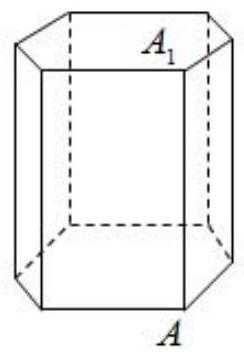
\includegraphics[max width=0.2\textwidth]{images/bo_d6dcisv7aajc739b5agg_111_619_1586_244_359_0.jpg}
\end{center}
\hspace*{3em} 

A. 4 B. 8 C. 12 D. 16

16. 设 \(D\) 是含数 1 的有限实数集, \(f\left( x\right)\) 是定义在 \(D\) 上的函数,若 \(f\left( x\right)\) 的图像绕原点逆时针旋转 \(\frac{\pi }{6}\) 后与原图像重合,则在以下各项中, \(f\left( 1\right)\) 的可能取值只能是 ( )

A. \(\sqrt{3}\) B. \(\frac{\sqrt{3}}{2}\) C. \(\frac{\sqrt{3}}{3}\) D. 0

\section*{三、解答题}

17. 已知圆锥的顶点为 \(P\) ,底面圆心为 \(O\) ,半径为 2 .

(1)设圆锥的母线长为 4，求圆锥的体积；

(2)设 \({PO} = 4,{OA}\) ， \({OB}\) 是底面半径，且 \(\angle {AOB} = {90}^{ \circ  }\) ， \(M\) 为线段 \({AB}\) 的中点，如图，求异面直线 \({PM}\) 与 \({OB}\) 所成的角的大小.

18. 设常数 \(a \in  R\) ,函数 \(f\left( x\right)  = a\sin {2x} + 2{\cos }^{2}x\) .

(1)若 \(f\left( x\right)\) 为偶函数，求 \(a\) 的值；

(2)若 \(f\left( \frac{\pi }{4}\right)  = \sqrt{3} + 1\) ，求方程 \(f\left( x\right)  = 1 - \sqrt{2}\) 在区间 \(\left\lbrack  {-\pi ,\pi }\right\rbrack\) 上的解.

19. 某群体的人均通勤时间, 是指单日内该群体中成员从居住地到工作地的平均用时, 某地上班族 \(S\) 中的成员仅以自驾或公交方式通勤，分析显示:当 \(S\) 中 \(x\% \left( {0 < x < {100}}\right)\) 的成员自驾时,自驾群体的人均通勤时间为 \(f\left( x\right)  = \left\{  \begin{array}{l} {30} \\  {2x} + \frac{1800}{x} - {90} \end{array}\right.\) (单位: 分钟),而公交群体的人均通勤时间不受 \(x\) 影响,恒为 40 分钟,试根据上述分析结果回答下列问题:

(1)当 \(x\) 在什么范围内时，公交群体的人均通勤时间少于自驾群体的人均通勤时间；

(2)求该地上班族 \(S\) 的人均通勤时间 \(g\left( x\right)\) 的表达式；讨论 \(g\left( x\right)\) 的单调性，并说明其实际意义.

20. 设常数 \(t > 2\) ,在平面直角坐标系 \({xOy}\) 中,已知点 \(F\left( {2,0}\right)\) ,直线 \(l : x = t\) ,曲线 \(\tau  : {y}^{2} = \; {8x}\left( {0 \leq  x \leq  t,y \geq  0}\right)\) ， \(l\) 与 \(x\) 轴交于点 \(A\) ，与 \(\tau\) 交于点 \(B\) ， \(P\) 、 \(Q\) 分别是曲线 \(\tau\) 与线段 \({AB}\) 上的动点.

(1) 用 \(t\) 为表示点 \(B\) 到点 \(F\) 的距离;

(2)设 \(t = 3\) ， \(\left| {FQ}\right|  = 2\) ，线段 \({OQ}\) 的中点在直线 \({FP}\) 上，求 \({AQP}\) 的面积；

(3) 设 \(t = 8\) ，是否存在以 \({FP}\) 、 \({FQ}\) 为邻边的矩形 \({FPEQ}\) ，使得点 \(E\) 在 \(\tau\) 上? 若存在，求点 \(P\) 的坐标; 若不存在, 说明理由.

21. 给定无穷数列 \(\left\{  {a}_{n}\right\}\) ，若无穷数列 \(\left\{  {b}_{n}\right\}\) 满足:对任意 \(n \in  {N}^{ * }\) ，都有 \(\left| {{b}_{n} - {a}_{n}}\right|  \leq  1\) ，则称 \(\left\{  {b}_{n}\right\}\) 与 \(\left\{  {a}_{n}\right\}\) “接近”.

(1)设 \(\left\{  {a}_{n}\right\}\) 是首项为 1，公比为 \(\frac{1}{2}\) 的等比数列， \({b}_{n} = {a}_{n + 1} + 1\) ， \(n \in  {N}^{ * }\) ，判断数列 \(\left\{  {b}_{n}\right\}\) 是否与 \(\left\{  {a}_{n}\right\}\) 接近,并说明理由

(2)设数列 \(\left\{  {a}_{n}\right\}\) 的前四项为: \({a}_{1} = 1,{a}_{2} = 2,{a}_{ = }4,{a}_{4} = 8\) ， \(\left\{  {b}_{n}\right\}\) 是一个与 \(\left\{  {a}_{n}\right\}\) 接近的数，记集合 \(M = \left\{  {x \mid   = {b}_{i},\mathrm{i} = 1,2,3,4}\right\}\) ,求 \(M\) 中元素的个数 \(m\)

(3)已知 \(\left\{  {a}_{n}\right\}\) 是公差为 \(d\) 的等差数列，若存在数列 \(\left\{  {b}_{n}\right\}\) 满足: \(\left\{  {b}_{n}\right\}\) 与 \(\left\{  {a}_{n}\right\}\) 接近，且在 \({b}_{2} - {b}_{1}\) ， \({b}_{3} - {b}_{2},\cdots ,{b}_{201} - {b}_{200}\) 中至少有 100 个为正数,求 \(d\) 的取值范围

\section*{2019 秋考}

一、填空题(本大题共有 12 题，满分 54 分，第 1\textasciitilde 6 题每题 4 分，第 7\textasciitilde 12 题每题 5 分) 1. 已知集合 \(A = \left( {-\infty ,3}\right) ,B = \left( {2, + \infty }\right)\) ，则 \(A \cap  B =\) \_\_\_\_\_.

2. 已知 \(z \in  C\) ,且满足 \(\frac{1}{z - 5} = \mathrm{i}\) ,求 \(z =\) \_\_\_\_\_.

3. 已知向量 \(\overrightarrow{a} = \left( {1,0,2}\right) ,\overrightarrow{b} = \left( {2,1,0}\right)\) ，则 \(\overrightarrow{a}\) 与 \(\overrightarrow{b}\) 的夹角为\_\_\_\_\_

4. 已知二项式 \({\left( 2x + 1\right) }^{5}\) ，则展开式中含 \({x}^{2}\) 项的系数为\_\_\_\_\_.

5. 已知 \(x,y\) 满足 \(\left\{  \begin{array}{l} x \geq  0 \\  y \geq  0 \\  x + y \leq  2 \end{array}\right.\) ,则 \(z = {2x} - {3y}\) 的最小值为\_\_\_\_\_.

6. 已知函数 \(f\left( x\right)\) 周期为 1,且当 \(0 < x \leq  1\) 时, \(f\left( x\right)  = {\log }_{2}x\) ,则 \(f\left( \frac{3}{2}\right)  =\) \_\_\_\_\_.

7. 若 \(x,y \in  {R}^{ + }\) ,且 \(\frac{1}{x} + {2y} = 3\) ,则 \(\frac{y}{x}\) 的最大值为\_\_\_\_\_.

8. 已知数列 \(\left\{  {a}_{n}\right\}\) 前 \(n\) 项和为 \({S}_{n}\) ，且满足 \({S}_{n} + {a}_{n} = 2\) ，则 \({S}_{5} =\) \_\_\_\_\_.

9. 过曲线 \({y}^{2} = {4x}\) 的焦点 \(F\) 并垂直于 \(x\) 轴的直线分别与曲线 \({y}^{2} = {4x}\) 交于 \(A,B,A\) 在 \(B\) 上方， \(M\) 为抛物线上一点， \(\overrightarrow{OM} = \lambda \overrightarrow{OA} + \left( {\lambda  - 2}\right) \overrightarrow{OB}\) ，则 \(\lambda  =\) \_\_\_\_\_.

10. 某三位数密码,每位数字可在 \(0 - 9\) 这 10 个数字中任选一个,则该三位数密码中,恰有两位数字相同的概率是\_\_\_\_\_.

11. 已知数列 \(\left\{  {a}_{n}\right\}\) 满足 \({a}_{n} < {a}_{n + 1}\left( {n \in  {N}^{ * }}\right) ,{P}_{n}\left( {n,{a}_{n}}\right) \left( {n \geq  3}\right)\) 均在双曲线 \(\frac{{x}^{2}}{6} - \frac{{y}^{2}}{2} = 1\) 上,则 \(\mathop{\lim }\limits_{{n \rightarrow   + \infty }}\left| {{P}_{n}{P}_{n + 1}}\right|  =\) \_\_\_\_\_.

12. 已知 \(f\left( x\right)  = \left| {\frac{2}{x - 1} - a}\right| \left( {{x1},a > 0}\right) ,f\left( x\right)\) 与 \(x\) 轴交点为 \(A\) ,若对于 \(f\left( x\right)\) 图象上任意一点 \(P\) ,在其图象上总存在另一点 \(Q\left( {P\text{ 、 }Q\text{ 异于 }A}\right)\) ,满足 \({AP} \bot  {AQ}\) ,且 \(\left| {AP}\right|  = \left| {AQ}\right|\) ,则 \(a =\) \_\_\_\_\_.

\section*{二、选择题 (本大题共有 4 题, 满分 20 分, 每题 5 分) 每题有且只有一个正确选项. 考生 应在答题纸的相应位置, 将代表正确选项的小方格涂黑.}

13. 已知直线方程 \({2x} - y + c = 0\) 的一个方向向量 \(\overrightarrow{d}\) 可以是 ( )

A. \(\left( {2, - 1}\right)\) B. \(\left( {2,1}\right)\) C. \(\left( {-1,2}\right)\) D. \(\left( {1,2}\right)\)

14. 一个直角三角形的两条直角边长分别为 1 和 2 , 将该三角形分别绕其两个直角边旋转得到的两个圆锥的体积之比为( )

A. 1 B. 2 C. 4 D. 8

15. 已知 \(\omega  \in  R\) ,函数 \(f\left( x\right)  = {\left( x - 6\right) }^{2} \cdot  \sin \left( {\omega x}\right)\) ,存在常数 \(a \in  R\) ,使 \(f\left( {x + a}\right)\) 为偶函数,则 \(\omega\) 的值可能为( )

A. \(\frac{\pi }{2}\) B. \(\frac{\pi }{3}\) C. \(\frac{\pi }{4}\) D. \(\frac{\pi }{5}\)

16. 已知 \(\tan \alpha  \cdot  \tan \beta  = \tan \left( {\alpha  + \beta }\right)\) . 有下列两个结论:

 \circled{1} 存在 \(\alpha\) 在第一象限， \(\beta\) 在第三象限；

 \circled{2} 存在 \(\alpha\) 在第二象限， \(\beta\) 在第四象限.

则( )

A.  \circled{1}  \circled{2} 均正确 B.  \circled{1}  \circled{2} 均错误 C.  \circled{1} 对， \circled{2} 错 D.  \circled{1} 错， \circled{2} 对

三、解答题 (本大题共有 5 题, 满分 76 分) 解答下列各题必须在答题纸的相应位置写出必要的步骤.

17. 如图，在长方体 \({ABCD} - {A}_{1}{B}_{1}{C}_{1}{D}_{1}\) 中， \(M\) 为 \(B{B}_{1}\) 上一点，已知 \({BM} = 2,{CD} = 3,{AD} =\) 4, \(A{A}_{1} = 5\) .

\begin{center}
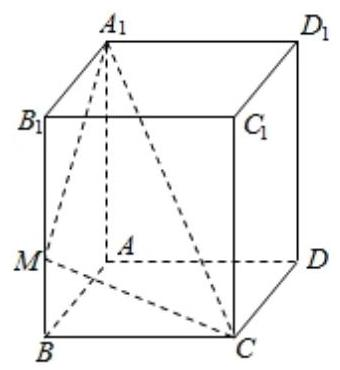
\includegraphics[max width=0.2\textwidth]{images/bo_d6dcisv7aajc739b5agg_117_261_695_340_370_0.jpg}
\end{center}
\hspace*{3em} 

(1)求直线 \({A}_{1}C\) 和平面 \({ABCD}\) 的夹角；

(2)求点 \(A\) 到平面 \({A}_{1}{MC}\) 的距离.

18. 已知 \(f\left( x\right)  = {ax} + \frac{1}{x + 1},a \in  R\) .

(1)当 \(a = 1\) 时，求不等式 \(f\left( x\right)  + 1 < f\left( {x + 1}\right)\) 的解集；

(2)若 \(f\left( x\right)\) 在 \(x \in  \left\lbrack  {1,2}\right\rbrack\) 时有零点,求 \(a\) 的取值范围.

19. 如图， \(A - B - C\) 为海岸线， \({AB}\) 为线段， \({BC}\) 为四分之一圆弧， \({BD} = {39.2}\mathrm{{km}}\) ， \(\angle {BDC} \; = {22}^{ \circ  },\;\angle {CBD} = {68}^{ \circ  },\;\angle {BDA} = {58}^{ \circ  }.\)

\begin{center}
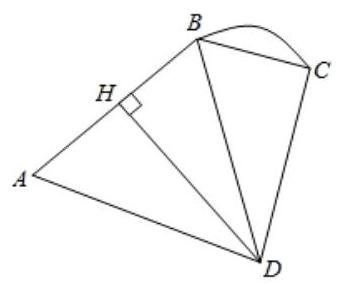
\includegraphics[max width=0.2\textwidth]{images/bo_d6dcisv7aajc739b5agg_118_261_221_343_285_0.jpg}
\end{center}
\hspace*{3em} 

(1)求 \({}^{ \circ  }{BC}\) 的长度；

(2)若 \({AB} = {40}\mathrm{\;{km}}\) ，求 \(D\) 到海岸线 \(A - B - C\) 的最短距离. (精确到 \({0.001}\mathrm{{km}}\) )

20. 已知椭圆 \(\frac{{x}^{2}}{8} + \frac{{y}^{2}}{4} = 1,{F}_{1},{F}_{2}\) 为左、右焦点,直线 \(l\) 过 \({F}_{2}\) 交椭圆于 \(A,B\) 两点.

(1)若直线 \(l\) 垂直于 \(x\) 轴,求 \(\left| {AB}\right|\) ；

(2)当 \(\angle {F}_{1}{AB} = {90}^{ \circ  }\) 时， \(A\) 在 \(x\) 轴上方时，求 \(A\) 、 \(B\) 的坐标；

(3)若直线 \(A{F}_{1}\) 交 \(y\) 轴于 \(M\) ，直线 \(B{F}_{1}\) 交 \(y\) 轴于 \(N\) ，是否存在直线 \(l\) ，使得 \({S}_{{F}_{1}{AB}} = {S}_{{F}_{1}{MN}}\) ，若存在,求出直线 \(l\) 的方程; 若不存在,请说明理由.

21. 数列 \(\left\{  {a}_{n}\right\}  \left( {n \in  {N}^{ * }}\right)\) 有 100 项, \({a}_{1} = a\) ,对任意 \(n \in  \left\lbrack  {2,{100}}\right\rbrack\) ,存在 \({a}_{n} = {a}_{i} + d,\mathrm{i} \in  \left\lbrack  {1,n - 1}\right\rbrack\) , 若 \({a}_{k}\) 与前 \(k - 1\) 项中某一项相等,则称 \({a}_{k}\) 具有性质 \(P\) .

(1) 若 \({a}_{1} = 1,d = 2\) ,求 \({a}_{4}\) 所有可能的值;

(2)若 \(\left\{  {a}_{n}\right\}\) 不为等差数列，求证:数列 \(\left\{  {a}_{n}\right\}\) 中存在某些项具有性质 \(P\) ；

(3)若 \(\left\{  {a}_{n}\right\}\) 中恰有三项具有性质 \(P\) ，这三项和为 \(c\) ，使用 \(a,d,c\) 表示 \({a}_{1} + {a}_{2} + \cdots  + {a}_{100}\) .

\section*{2019 春考}

一、填空题 (本大题共 12 题,满分 54 分,第 \(1 - 6\) 题每题 4 分,第 7-12 题每题 5 分) 1. 已知集合 \(A = \{ 1,2,3,4,5\} ,B = \{ 3,5,6\}\) ，则 \(A \cap  B =\) \_\_\_\_\_.

2. 计算 \(\mathop{\lim }\limits_{{n \rightarrow  \infty }}\frac{2{n}^{2} - {3n} + 1}{{n}^{2} - {4n} + 1} =\) \_\_\_\_\_.

3. 不等式 \(\left| {x + 1}\right|  < 5\) 的解集为\_\_\_\_\_.

4. 函数 \(f\left( x\right)  = {x}^{2}\left( {x0}\right)\) 的反函数为\_\_\_\_\_.

5. 设 \(\mathrm{i}\) 为虚数单位, \(3\bar{z} - \mathrm{i} = 6 + 5\mathrm{i}\) ,则 \(\left| z\right|\) 的值为\_\_\_\_\_.

6. 已知 \(\left\{  \begin{array}{l} {2x} + {2y} =  - 1 \\  {4x} + {a}^{2}y = a \end{array}\right.\) ,当方程有无穷多解时, \(a\) 的值为\_\_\_\_\_.

7. 在 \({\left( x + 1\sqrt{x}\right) }^{6}\) 的展开式中，常数项等于\_\_\_\_\_.

8. 在 \({ABC}\) 中， \({AC} = 3,\;3\sin A = 2\sin B\) ，且 \(\cos C = {14}\) ，则 \({AB} =\) \_\_\_\_\_.

9. 首届中国国际进口博览会在上海举行，某高校拟派 4 人参加连续 5 天的志愿者活动，其中甲连续参加 2 天，其他人各参加 1 天，则不同的安排方法有\_\_\_\_\_种(结果用数值表示).

10. 如图,已知正方形 \({OABC}\) ,其中 \({OA} = a\left( {a1}\right)\) ,函数 \(y = 3{x}^{2}\) 交 \({BC}\) 于点 \(P\) ,函数 \(y = {x}^{-{12}}\) 交 \({AB}\) 于点 \(Q\) ，当 \(\left| {AQ}\right|  + \left| {CP}\right|\) 最小时，则 \(a\) 的值为\_\_\_\_\_.

\begin{center}
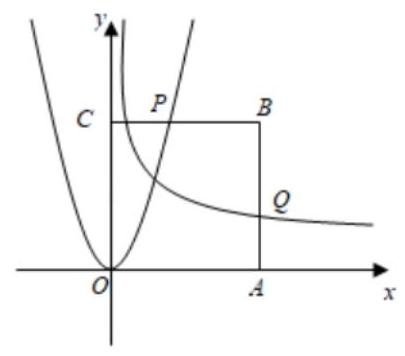
\includegraphics[max width=0.3\textwidth]{images/bo_d6dcisv7aajc739b5agg_120_259_1243_405_356_0.jpg}
\end{center}
\hspace*{3em} 

11. 在椭圆 \(4 + 2 = 1\) 上任意一点 \(P,Q\) 与 \(P\) 关于 \(x\) 轴对称,若有 \(\overrightarrow{{F}_{1}P} \cdot  \overrightarrow{{F}_{2}P} \leq  1\) ,则 \(\overrightarrow{{F}_{1}P}\) 与 \(\overrightarrow{{F}_{2}Q}\) 的夹角范围为\_\_\_\_\_.

12. 已知集合 \(A = \left\lbrack  {t,t + 1}\right\rbrack   \cup  \left\lbrack  {t + 4,t + 9}\right\rbrack  ,\;0 \notin  A\) ，存在正数 \(\lambda\) ，使得对任意 \(a \in  A\) ，都有 \({\lambda a} \in \; A\) ，则 \(t\) 的值是\_\_\_\_\_.

\section*{二、选择题 (本大题共 4 题, 每题 5 分, 共 20 分)}

13. 下列函数中，值域为 \(\lbrack 0, + \infty )\) 的是( )

A. \(y = {2}^{x}\) B. \(y = {x}^{12}\) C. \(y = \tan x\) D. \(y = \cos x\)

14. 已知 \(a\text{ 、 }b \in  R\) ，则 “ \({a}^{2} > {b}^{2}\) ” 是 “ \(\left| a\right|  > \left| b\right|\) ” 的( )

A. 充分非必要条件 B. 必要非充分条件

C. 充要条件 D. 既非充分又非必要条件

15. 已知平面 \(\alpha \text{ 、 }\beta \text{ 、 }\gamma\) 两两垂直，直线 \(a\text{ 、 }b\text{ 、 }c\) 满足: \(a \subseteq  \alpha\) ， \(b \subseteq  \beta\) ， \(c \subseteq  \gamma\) ，则直线 \(a\text{ 、 }b\) 、 \(c\) 不可能满足以下哪种关系 ( )

A. 两两垂直 B. 两两平行 C. 两两相交 D. 两两异面

16. 以 \(\left( {{a}_{1},0}\right) ,\left( {{a}_{2},0}\right)\) 为圆心的两圆均过 \(\left( {1,0}\right)\) ,与 \(y\) 轴正半轴分别交于 \(\left( {0,{y}_{1}}\right) ,\left( {0,{y}_{2}}\right)\) ,且满足 \(\ln {y}_{1} + \ln {y}_{2} = 0\) ，则点 \(\left( {1{a}_{1},1{a}_{2}}\right)\) 的轨迹是( )

A. 直线 B. 圆 C. 椭圆 D. 双曲线

三、解答题 (本大题共 5 题, 共 \({14} + {14} + {14} + {16} + {18} = {76}\) 分)

17. 如图,在正三棱锥 \(P - {ABC}\) 中, \({PA} = {PB} = {PC} = 2,{AB} = {BC} = {AC} = \sqrt{3}\) .

\begin{center}
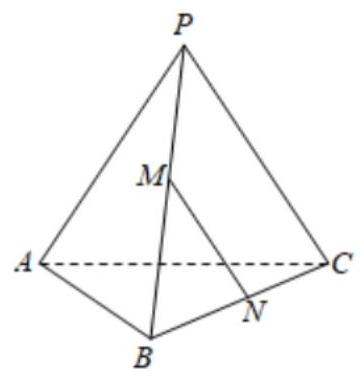
\includegraphics[max width=0.2\textwidth]{images/bo_d6dcisv7aajc739b5agg_122_261_319_364_377_0.jpg}
\end{center}
\hspace*{3em} 

(1)若 \({PB}\) 的中点为 \(M,{BC}\) 的中点为 \(N\) ，求 \({AC}\) 与 \({MN}\) 的夹角；

(2) 求 \(P - {ABC}\) 的体积.

18. 已知数列 \(\left\{  {a}_{n}\right\}  ,{a}_{1} = 3\) ,前 \(n\) 项和为 \({S}_{n}\) .

(1)若 \(\left\{  {a}_{n}\right\}\) 为等差数列，且 \({a}_{4} = {15}\) ，求 \({S}_{n}\) ；

( 2 )若 \(\left\{  {a}_{n}\right\}\) 为等比数列，且 \(\mathop{\lim }\limits_{{n \rightarrow  \infty }}{S}_{n} < {12}\) ，求公比 \(q\) 的取值范围.

19. 改革开放 40 年, 我国卫生事业取得巨大成就, 卫生总费用增长了数十倍. 卫生总费用包括个人现在支出、社会支出、政府支出，如表为 2012 年 2015 年我国卫生货用中个人现金支出、社会支出和政府支出的费用 (单位:亿元) 和在卫生总费用中的占比.

\begin{center}
\adjustbox{max width=\textwidth}{
\begin{tabular}{|c|c|c|c|c|c|c|c|}
\hline
\multirow{2}{*}{年份} & \multirow{2}{*}{卫生总费用 (亿元)} & \multicolumn{2}{|c|}{个人现金卫生支出} & \multicolumn{2}{|c|}{社会卫生支出} & \multicolumn{2}{|c|}{政府卫生支出} \\
\cline{3-8}
 &  & 绝对数 (亿元) & 占卫生总费用比重 (\%) & 绝对数 (亿元) & 占卫生总费用比重 (\%) & 绝对数 (亿元) & 占卫生总费用比重 (\%) \\
\cline{1-8}
\makecell{ 20 \\ 12 } & 288119.00 & 9656.32 & 34.34 & 100030.70 & 35.67 & 8431.98 & 29.99 \\
\cline{1-8}
\makecell{ 20 \\ 13 } & 31668.95 & 10729.34 & 33.88 & 11393.79 & 35.98 & 9545.81 & 30.14 \\
\cline{1-8}
\makecell{ 20 \\ 14 } & 35312.40 & 11295.41 & 31.99 & 13437.75 & 38.05 & 10579.25 & 29.96 \\
\cline{1-8}
\makecell{ 20 \\ 15 } & 40974.64 & 11992.65 & 29.27 & 16506.71 & 40.29 & 12475.28 & 30.45 \\
\cline{1-8}
\hline
\end{tabular}
}
\end{center}

(数据来源于国家统计年鉴)

(1)指出 2012 年到 2015 年之间我国卫生总费用中个人现金支出占比和社会支出占比的变化趋势:

(2)设 \(t = 1\) 表示 1978 年，第 \(n\) 年卫生总费用与年份 \(t\) 之间拟合函数 \(f\left( t\right)  = \frac{357876.6053}{1 + {\mathrm{e}}^{{6.4420} - {0.1136t}}}\) 研究函数 \(f\left( t\right)\) 的单调性,并预测我国卫生总费用首次超过 12 万亿的年份.

20. 已知抛物线方程 \({y}^{2} = {4x}\) ， \(F\) 为焦点， \(P\) 为抛物线准线上一点， \(Q\) 为线段 \({PF}\) 与抛物线的交点,定义: \(d\left( P\right)  = \frac{\left| PF\right| }{\left| FQ\right| }\) .

(1)当 \(P\left( {-1, - {83}}\right)\) 时，求 \(d\left( P\right)\) ；

(2)证明:存在常数 \(a\) ，使得 \({2d}\left( P\right)  = \left| {PF}\right|  + a\) ；

(3) \({P}_{1},{P}_{2},{P}_{3}\) 为抛物线准线上三点，且 \(\left| {{P}_{1}{P}_{2}}\right|  = \left| {{P}_{2}{P}_{3}}\right|\) ，判断 \(d\left( {P}_{1}\right)  + d\left( {P}_{3}\right)\) 与 \({2d}\left( {P}_{2}\right)\) 的关系.

21. 已知等差数列 \(\left\{  {a}_{n}\right\}\) 的公差 \(d \in  (0,\pi \rbrack\) ,数列 \(\left\{  {b}_{n}\right\}\) 满足 \({b}_{n} = \sin \left( {a}_{n}\right)\) ,集合 \(S = \; \left\{  {x \mid  x = {b}_{n},n \in  {N}^{ * }}\right\}  .\)

(1)若 \({a}_{1} = 0,d = 3\) 求集合 \(S\) ；

(2)若 \({a}_{1} = {\pi 2}\) ，求 \(d\) 使得集合 \(S\) 恰好有两个元素；

(3)若集合 \(S\) 恰好有三个元素: \({b}_{n + T} = {b}_{n}\) ， \(T\) 是不超过 7 的正整数，求 \(T\) 的所有可能的值.

\section*{2020 秋考}

一、填空题 (本题共 12 小题,满分 54 分,其中 \(1 - 6\) 题每题 4 分, \(7 - {12}\) 题每题 5 分) 1. 已知集合 \(A = \{ 1,2,4\} ,B = \{ 2,3,4\}\) ，求 \(A \cap  B =\) \_\_\_\_\_.

2. \(\mathop{\lim }\limits_{{n \rightarrow  \infty }}\frac{n + 1}{{3n} - 1} =\) \_\_\_\_\_.

3. 已知复数 \(z\) 满足 \(z = 1 - 2\mathrm{i}\) ( \(\mathrm{i}\) 为虚数单位),则 \(\left| z\right|  =\) \_\_\_\_\_.

4. 已知行列式 \(\left| \begin{array}{l} 1 \\  2 \\  3 \end{array}\right|  = 6\) ，则行列式 \(\left| \begin{array}{l} a \\  d \end{array}\right|  =\) \_\_\_\_\_.

5. 已知 \(f\left( x\right)  = {x}^{3}\) ,则 \({f}^{-1}\left( x\right)  =\) \_\_\_\_\_.

6. 已知 \(a\text{ 、 }b\text{ 、 }1\text{ 、 }2\) 的中位数为3,平均数为4,则 \({ab} =\) \_\_\_\_\_.

7. 已知 \(\left\{  \begin{array}{l} x + y \geq  2 \\  y \geq  0 \\  x + {2y} - 3 \leq  0 \end{array}\right.\) 则 \(z = y - {2x}\) 的最大值为\_\_\_\_\_.

8. 已知 \(\left\{  {a}_{n}\right\}\) 是公差不为零的等差数列,且 \({a}_{1} + {a}_{10} = {a}_{9}\) ,则 \(\frac{{a}_{1} + {a}_{2} + \cdots  + {a}_{9}}{{a}_{10}} =\) \_\_\_\_\_.

9. 从 6 人中挑选 4 人去值班，每人值班 1 天，第一天需要 1 人，第二天需要 1 人，第三天需要 2 人，则有\_\_\_\_\_种排法.

10. 椭圆 \(\frac{{x}^{2}}{4} + \frac{{y}^{2}}{3} = 1\) ,过右焦点 \(F\) 作直线 \(l\) 交椭圆于 \(P\text{ 、 }Q\) 两点， \(P\) 在第二象限已知 \(Q\left( {{x}_{Q},{y}_{Q}}\right) ,\;{Q}^{\prime }\left( {{x}_{Q}^{\prime },{y}_{Q}^{\prime }}\right)\) 都在椭圆上,且 \({y}_{Q} + {y}_{Q}^{\prime } = 0,\;F{Q}^{\prime } \bot  {PQ}\) ,则直线 \(l\) 的方程为\_\_\_\_\_.

11. 设 \(a \in  R\) ,若存在定义域 \(R\) 的函数 \(f\left( x\right)\) 既满足 “对于任意 \({x}_{0} \in  R,f\left( {x}_{0}\right)\) 的值为 \({x}_{0}^{2}\) 或 \({x}_{0}\) ” 又满足 “关于 \(x\) 的方程 \(f\left( x\right)  = a\) 无实数解”,则 \(a\) 的取值范围为\_\_\_\_\_.

12. 已知 \({\overrightarrow{a}}_{1},{\overrightarrow{a}}_{2},{\overrightarrow{b}}_{1},{\overrightarrow{b}}_{2},\cdots ,{\overrightarrow{b}}_{k}\left( {k \in  {N}^{ * }}\right)\) 是平面内两两互不相等的向量,满足 \(\left| {{\overrightarrow{a}}_{1} - {\overrightarrow{a}}_{2}}\right|  = 1\) , 且 \(\left| {{\overrightarrow{a}}_{i} - {\overrightarrow{b}}_{j}}\right|  \in  \{ 1,2\}\) (其中 \(\mathrm{i} = 1,2,j = 1,2,\cdots ,k)\) ，则 \(k\) 的最大值为\_\_\_\_\_.

\section*{二、选择题 (本题共有 4 小题,每题 5 分,共计 20 分)}

13. 下列不等式恒成立的是( )

A. \({a}^{2} + {b}^{2} \leq  {2ab}\) B. \({a}^{2} + {b}^{2} \geq   - {2ab}\) C. \(a + b \geq   - 2\sqrt{\left| ab\right| }\) D. \(a + b \leq  2\sqrt{\left| ab\right| }\)

14. 已知直线 \(l\) 的解析式为 \({3x} + {4y} + 1 = 0\) ，则下列各式是 \(l\) 的参数方程的是 ( )

A. \(\left\{  \begin{array}{l} x = 1 + {3t} \\  y =  - 1 - {4t} \end{array}\right.\) B. \(\left\{  \begin{array}{l} x = 1 - {4t} \\  y =  - 1 + {3t} \end{array}\right.\) C. \(\left\{  \begin{array}{l} x = 1 - {3t} \\  y =  - 1 + {4t} \end{array}\right.\) D. \(\left\{  \begin{array}{l} x = 1 + {4t} \\  y = 1 - {3t} \end{array}\right.\)

15. 在棱长为 10 的正方体 \({ABCD} - {A}_{1}{B}_{1}{C}_{1}{D}_{1}\) 中， \(P\) 为左侧面 \({AD}{D}_{1}{A}_{1}\) 上一点，已知点 \(P\) 到 \({A}_{1}{D}_{1}\) 的距离为 3,点 \(P\) 到 \(A{A}_{1}\) 的距离为 2,则过点 \(P\) 且与 \({A}_{1}C\) 平行的直线交正方体于 \(P\) 、 \(Q\) 两点,则 \(Q\) 点所在的平面是(   )

\begin{center}
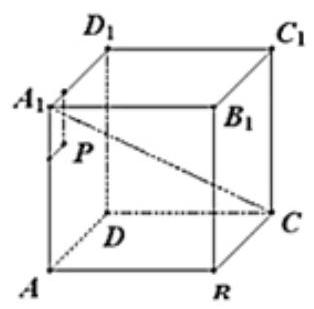
\includegraphics[max width=0.2\textwidth]{images/bo_d6dcisv7aajc739b5agg_126_280_1510_314_309_0.jpg}
\end{center}
\hspace*{3em} 

A. \(A{A}_{1}{B}_{1}B\) B. \(B{B}_{1}{C}_{1}C\) C. \(C{C}_{1}{D}_{1}D\) D. \({ABCD}\)

16. 若存在 \(a \in  R\) 且 \(a \neq  0\) ,对任意的 \(x \in  R\) ,均有 \(f\left( {x + a}\right)  < f\left( x\right)  + f\left( a\right)\) 恒成立,则称函数 \(f\left( x\right)\) 具有性质 \(P\) ,已知: \({q}_{1} : f\left( x\right)\) 单调递减,且 \(f\left( x\right)  > 0\) 恒成立; \({q}_{2} : f\left( x\right)\) 单调递增,存在 \({x}_{0} < 0\) 使得 \(f\left( {x}_{0}\right)  = 0\) ,则是 \(f\left( x\right)\) 具有性质 \(P\) 的充分条件是 ( )

A. 只有 \({q}_{1}\) B. 只有 \({q}_{2}\) C. \({q}_{1}\) 和 \({q}_{2}\) D. \({q}_{1}\) 和 \({q}_{2}\) 都不是

\section*{三、解答题 (本题共 5 小题, 共计 76 分)}

17. 已知边长为 1 的正方形 \({ABCD}\) ,沿 \({BC}\) 旋转一周得到圆柱体.

(1)求圆柱体的表面积；

(2)正方形 \({ABCD}\) 绕 \({BC}\) 逆时针旋转 \(\frac{\pi }{2}\) 到 \({A}_{1}{BC}{D}_{1}\) ，求 \(A{D}_{1}\) 与平面 \({ABCD}\) 所成的角.

18. 已知 \(f\left( x\right)  = \sin {\omega x}\left( {\omega 0}\right)\) .

(1) 若 \(f\left( x\right)\) 的周期是 \({4\pi }\) ,求 \(\omega\) ,并求此时 \(f\left( x\right)  = \frac{1}{2}\) 的解集;

(2) 已知 \(\omega  = 1,g\left( x\right)  = {f}^{2}\left( x\right)  + \sqrt{3}f\left( {-x}\right) f\left( {\frac{\pi }{2} - x}\right) ,x \in  \left\lbrack  {0,\frac{\pi }{4}}\right\rbrack\) ,求 \(g\left( x\right)\) 的值域.

19. 已知: \(v = \frac{q}{x},\;x \in  (0,{80}\rbrack\) ,且 \(v = \left\{  \begin{array}{l} {100} - {135}{\left( \frac{1}{3}\right) }^{\frac{80}{x}}, \\   - k\left( {x - {40}}\right)  + {85}, \end{array}\right.\)

(1)若 \(v > {95}\) ，求 \(x\) 的取值范围；

(2)已知 \(x = {80}\) 时， \(v = {50}\) ，求 \(x\) 为多少时， \(q\) 可以取得最大值，并求出该最大值.

20. 双曲线 \({C}_{1} : \frac{{x}^{2}}{4} - \frac{{y}^{2}}{{b}^{2}} = 1\) ,圆 \({C}_{2} : {x}^{2} + {y}^{2} = 4 + {b}^{2}\left( {b0}\right)\) 在第一象限交点为 \(A,A\left( {{x}_{A},{y}_{A}}\right)\) ,

曲线 \(\Gamma \left\{  \begin{array}{l} \frac{{x}^{2}}{4} - \frac{{y}^{2}}{{b}^{2}} = 1, \\  {x}^{2} + {y}^{2} = 4 + {b}^{2}, \end{array}\right.\)

\begin{center}
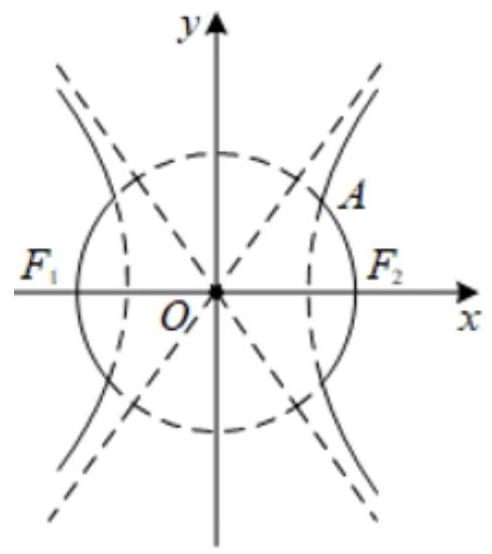
\includegraphics[max width=0.3\textwidth]{images/bo_d6dcisv7aajc739b5agg_128_253_339_492_554_0.jpg}
\end{center}
\hspace*{3em} 

(1)若 \({x}_{A} = \sqrt{6}\) ，求 \(b\) ；

(2)若 \(b = \sqrt{5}\) ， \({C}_{2}\) 与 \(x\) 轴交点记为 \({F}_{1}\) 、 \({F}_{2}\) ， \(P\) 是曲线 \(\Gamma\) 上一点，且在第一象限，并满足 \(\left| {P{F}_{1}}\right| \; = 8\) ,求 \(\angle {F}_{1}P{F}_{2}\) ;

(3)过点 \(S\left( {0,2 + \frac{{b}^{2}}{2}}\right)\) 且斜率为 \(- \frac{b}{2}\) 的直线 \(l\) 交曲线 \(\Gamma\) 于 \(M\text{ 、 }N\) 两点，用 \(b\) 的代数式表示 \(\overrightarrow{OM}\) . \(\overrightarrow{ON}\) ，并求出 \(\overrightarrow{OM} \cdot  \overrightarrow{ON}\) 的取值范围.

21. 有限数列 \(\left\{  {a}_{n}\right\}\) ,若满足 \(\left| {{a}_{1} - {a}_{2}}\right|  \leq  \left| {{a}_{1} - {a}_{3}}\right|  \leq  \cdots  \leq  \left| {{a}_{1} - {a}_{m}}\right| ,m\) 是项数,则称 \(\left\{  {a}_{n}\right\}\) 满足性质 \(p\) .

(1)判断数列3，2,5,1和4,3,2,5,1是否具有性质 \(p\) ，请说明理由;

(2)若 \({a}_{1} = 1\) ，公比为 \(q\) 的等比数列，项数为 10，具有性质 \(p\) ，求 \(q\) 的取值范围；

(3)若 \({a}_{n}\) 是 \(1,2,\cdots ,m\) 的一个排列 \(\left( {m \geq  4}\right) ,{b}_{k} = {a}_{k + 1}\left( {k = 1,2\cdots ,m - 1}\right) ,\left\{  {a}_{n}\right\}  ,\left\{  {b}_{n}\right\}\) 都具有性质 \(p\) ,求所有满足条件的 \(\left\{  {a}_{n}\right\}\) .

\section*{2020 春考}

一、填空题(本大题共 12 题，满分 54 分，第 1\textasciitilde 6 题每题 4 分，第 7-12 题每题 5 分) 1. 集合 \(A = \{ 1,3\} ,B = \{ 1,2,a\}\) ，若 \(A \subseteq  B\) ，则 \(a =\) \_\_\_\_\_.

2. 不等式 \({1x} > 3\) 的解集为\_\_\_\_\_.

3. 函数 \(y = \tan {2x}\) 的最小正周期为\_\_\_\_\_.

4. 已知复数 \(z\) 满足 \(z + 2\bar{z} = 6 + \mathrm{i}\) ，则 \(z\) 的实部为\_\_\_\_\_.

5. 已知 \(3\sin {2x} = 2\sin x,x \in  \left( {0,\pi }\right)\) ，则 \(x =\) \_\_\_\_\_.

6. 若函数 \(y = a \cdot  {3}^{x} + {13}^{x}\) 为偶函数，则 \(a =\) \_\_\_\_\_.

7. 已知直线 \({l}_{1} : x + {ay} = 1,{l}_{2} : {ax} + y = 1\) ，若 \({l}_{1}//{l}_{2}\) ，则 \({l}_{1}\) 与 \({l}_{2}\) 的距离为\_\_\_\_\_.

8. 已知二项式 \({\left( 2x + \sqrt{x}\right) }^{5}\) ，则展开式中 \({x}^{3}\) 的系数为\_\_\_\_\_.

9. 三角形 \({ABC}\) 中， \(D\) 是 \({BC}\) 中点， \({AB} = 2,{BC} = 3,{AC} = 4\) ，则 \(\overrightarrow{AD} \cdot  \overrightarrow{AB} =\) \_\_\_\_\_.

10. 已知 \(A = \{  - 3, - 2, - 1,0,1,2,3\} ,a\text{ 、 }b \in  A\) ，则 \(\left| a\right|  < \left| b\right|\) 的情况有\_\_\_\_\_种.

11. 已知 \({A}_{1}\text{ 、 }{A}_{2}\text{ 、 }{A}_{3}\text{ 、 }{A}_{4}\text{ 、 }{A}_{5}\) 五个点,满足 \(\overrightarrow{{A}_{n}{A}_{n + 1}} \cdot  \overrightarrow{{A}_{n + 1}{A}_{n + 2}} = 0\left( {n = 1,2,3}\right) ,\left| \overrightarrow{{A}_{n}{A}_{n + 1}}\right|\) . \(\left| \overrightarrow{{A}_{n + 1}{A}_{n + 2}}\right|  = n + 1\left( {n = 1,2,3}\right)\) ，则 \(\left| \overrightarrow{{A}_{1}{A}_{5}}\right|\) 的最小值为\_\_\_\_\_.

12. 已知 \(f\left( x\right)  = \sqrt{x - 1}\) ,其反函数为 \({f}^{-1}\left( x\right)\) ,若 \({f}^{-1}\left( x\right)  - a = f\left( {x + a}\right)\) 有实数根,则 \(a\) 的取值范围为\_\_\_\_\_.

\section*{二、选择题 (本大题共 4 题, 每题 5 分, 共 20 分)}

13. 计算: \(\mathop{\lim }\limits_{{n \rightarrow  \infty }}\frac{{3}^{n} + {5}^{n}}{{3}^{n - 1} + {5}^{n - 1}} =\) (   )

A. 3 B. 53 C. 35 D. 5

14. ” \(\alpha  = \beta\) ” 是 “ \({\sin }^{2}\alpha  + {\cos }^{2}\beta  = 1\) ” 的 ( )

A. 充分非必要条件 B. 必要非充分条件

C. 充要条件 D. 既非充分又非必要条件

15. 已知椭圆 \(2 + {y}^{2} = 1\) ，作垂直于 \(x\) 轴的垂线交椭圆于 \(A\) 、 \(B\) 两点，作垂直于 \(y\) 轴的垂线交椭圆于 \(C\) 、 \(D\) 两点,且 \({AB} = {CD}\) ，两垂线相交于点 \(P\) ，则点 \(P\) 的轨迹是 ( )

A. 椭圆 B. 双曲线 C. 圆 D. 抛物线

16. 数列 \(\left\{  {a}_{n}\right\}\) 各项均为实数,对任意 \(n \in  {N}^{ * }\) 满足 \({a}_{n + 3} = {a}_{n}\) ,且行列式 \(\left| \begin{matrix} {a}_{n} & {a}_{n + 1} \\  {a}_{n + 2} & {a}_{n + 3} \end{matrix}\right|  = c\) 为定值, 则下列选项中不可能的是 ( )

A. \({a}_{1} = 1,c = 1\) B. \({a}_{1} = 2,c = 2\) C. \({a}_{1} =  - 1,c = 4\) D. \({a}_{1} = 2,c = 0\)

\section*{三、解答题 (本大题共 5 题, 共 \({14} + {14} + {14} + {16} + {18} = {76}\) 分)}

17. 已知四棱锥 \(P - {ABCD}\) ，底面 \({ABCD}\) 为正方形，边长为3， \({PD}\bot\) 平面 \({ABCD}\) .

\begin{center}
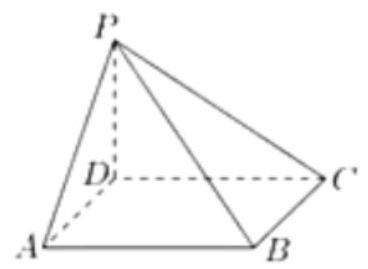
\includegraphics[max width=0.2\textwidth]{images/bo_d6dcisv7aajc739b5agg_132_263_223_368_269_0.jpg}
\end{center}
\hspace*{3em} 

(1)若 \({PC} = 5\) ，求四棱锥 \(P - {ABCD}\) 的体积；

(2)若直线 \({AD}\) 与 \({BP}\) 的夹角为 \({60}^{ \circ  }\) ，求 \({PD}\) 的长.

18. 已知各项均为正数的数列 \(\left\{  {a}_{n}\right\}\) ,其前 \(n\) 项和为 \({S}_{n},{a}_{1} = 1\) .

(1)若数列 \(\left\{  {a}_{n}\right\}\) 为等差数列， \({S}_{10} = {70}\) ，求数列 \(\left\{  {a}_{n}\right\}\) 的通项公式；

(2)若数列 \(\left\{  {a}_{n}\right\}\) 为等比数列， \({a}_{4} = {18}\) ，求满足 \({S}_{n} > {{100}{a}_{n}}\) 时 \(n\) 的最小值.

19. 有一条长为 120 米的步行道 \({OA},A\) 是垃圾投放点 \({\omega }_{1}\) ,若以 \(O\) 为原点, \({OA}\) 为 \(x\) 轴正半轴建立直角坐标系,设点 \(B\left( {x,0}\right)\) ,现要建设另一座垃圾投放点 \({\omega }_{2}\left( {t,0}\right)\) ,函数 \({f}_{t}\left( x\right)\) 表示与点 \(B\) 距离最近的垃圾投放点的距离.

(1) 若 \(t = {60}\) ,求 \({f}_{60}\left( {10}\right) \text{ 、 }{f}_{60}\left( {80}\right) \text{ 、 }{f}_{60}\left( {95}\right)\) 的值,并写出 \({f}_{60}\left( x\right)\) 的函数解析式;

( 2 )若可以通过 \({f}_{t}\left( x\right)\) 与坐标轴围成的面积来测算扔垃圾的便利程度，面积越小越便利. 问:垃圾投放点 \({\omega }_{2}\) 建在何处才能比建在中点时更加便利?

20. 已知抛物线 \({y}^{2} = x\) 上的动点 \(M\left( {{x}_{0},{y}_{0}}\right)\) ,过 \(M\) 分别作两条直线交抛物线于 \(P\text{ 、 }Q\) 两点,交直线 \(x = t\) 于 \(A\text{ 、 }B\) 两点.

(1)若点 \(M\) 纵坐标为 \(\sqrt{2}\) ，求 \(M\) 与焦点的距离；

(2)若 \(t =  - 1,P\left( {1,1}\right) ,Q\left( {1, - 1}\right)\) ，求证: \({y}_{A} \cdot  {y}_{B}\) 为常数；

(3) 是否存在 \(t\) ,使得 \({y}_{A} \cdot  {y}_{B} = 1\) 且 \({y}_{P} \cdot  {y}_{Q}\) 为常数? 若存在,求出 \(t\) 的所有可能值,若不存在,请说明理由.

21. 已知非空集合 \(A \subseteq  R\) ，函数 \(y = f\left( x\right)\) 的定义域为 \(D\) ，若对任意 \(t \in  A\) 且 \(x \in  D\) ，不等式 \(f\left( x\right) \; \leq  f\left( {x + t}\right)\) 恒成立,则称函数 \(f\left( x\right)\) 具有 \(A\) 性质.

(1) 当 \(A = \{  - 1\}\) ,判断 \(f\left( x\right)  =  - x\text{ 、 }g\left( x\right)  = {2x}\) 是否具有性质;

(2) 当 \(A = \left( {0,1}\right) ,f\left( x\right)  = x + {1x},x \in  \lbrack a, + \infty )\) ,若 \(f\left( x\right)\) 具有 \(A\) 性质,求 \(a\) 的取值范围;

(3) 当 \(A = \{  - 2,m\} ,m \in  Z\) ,若 \(D\) 为整数集且具有 \(A\) 性质的函数均为常值函数,求所有符合条件的 \(m\) 的值.

\section*{2021 秋考}

一、填空题(本大题共 12 题，满分 54 分，第 \(1 \sim  6\) 题每题 4 分，第 \(7 \sim  {12}\) 题每题 5 分)

1. 已知 \({z}_{1} = 1 + \mathrm{i},{z}_{2} = 2 + 3\mathrm{i}\) ，则 \({z}_{1} + {z}_{2} =\) \_\_\_\_\_.

2. 已知 \(A = \{ x \mid  {2x} \leq  1\} ,B = \{  - 1,0,1\}\) ，则 \(A \cap  B =\) \_\_\_\_\_.

3. 已知圆 \({x}^{2} + {y}^{2} - {2x} - {4y} = 0\) ，则该圆的圆心坐标为\_\_\_\_\_.

4. 正方形 \({ABCD}\) 的边长为 3，则 \(\overrightarrow{AB} \cdot  \overrightarrow{AC} =\) \_\_\_\_\_.

\begin{center}
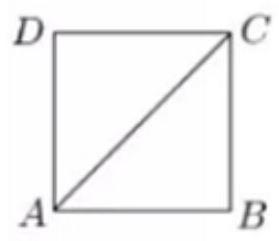
\includegraphics[max width=0.2\textwidth]{images/bo_d6dcisv7aajc739b5agg_134_261_1351_279_241_0.jpg}
\end{center}
\hspace*{3em} 

5. 已知 \(f\left( x\right)  = \frac{3}{x} + 2\) ，则 \({f}^{-1}\left( 1\right)  =\) \_\_\_\_\_.

6. 已知二项式 \({\left( x + a\right) }^{5}\) 展开式中， \({x}^{2}\) 项的系数为 80 ，则 \(a =\) \_\_\_\_\_.

7. 已知实数 \(x\) 、 \(y\) 满足 \(\left\{  \begin{array}{l} x \leq  3 \\  {2x} - y - 2 \geq  0 \\  {3x} + y - 8 \geq  0 \end{array}\right.\) ，则 \(z = x - y\) 的最大值为\_\_\_\_\_.

8. 已知无穷等比数列 \(\left\{  {a}_{n}\right\}\) 和 \(\left\{  {b}_{n}\right\}\) ,满足 \({a}_{1} = 3,{b}_{n} = {a}_{2n},{a}_{n}\) 的各项和为 9,则数列 \(\left\{  {b}_{n}\right\}\) 的各项和为\_\_\_\_\_.

9. 已知圆柱的底面半径为 1,高为 \(2,{AB}\) 为上底面圆的一条直径， \(C\) 为下底面圆周上的一个动点,则 \({ABC}\) 的面积的取值范围为\_\_\_\_\_.

10. 已知花博会有四个不同的场馆 \(A\) 、 \(B\) 、 \(C\) 、 \(D\) ，甲、乙两人每人选 2 个去参观，则他们的选择中，恰有一个场馆相同的概率为\_\_\_\_\_.

11. 已知抛物线: \({y}^{2} = {2px}\left( {p0}\right)\) ,若第一象限的 \(A,B\) 两点在抛物线上,焦点为 \(F,\left| {AF}\right|  = 2\) , \(\left| {BF}\right|  = 4\) ， \(\left| {AB}\right|  = 3\) ，则直线 \({AB}\) 的斜率为\_\_\_\_\_.

12. 已知 \(a \in  {N}^{ * }\left( {\mathrm{i} = 1,2,,9}\right)\) ,对任意的 \(k \in  {N}^{ * }\left( {2 \leq  k \leq  8}\right) ,{a}_{k} = {a}_{k - 1} + 1\) 或 \({a}_{k} = {a}_{k + 1} - 1\) 中有且仅有一个成立,且 \({a}_{1} = 6,{a}_{9} = 9\) ,则 \({a}_{1} +  + {a}_{9}\) 的最小值为\_\_\_\_\_.

\section*{二、选择题 (本大题共 4 题,每题 5 分, 共 20 分)}

13. 下列函数中, 既是奇函数又是减函数的是 ( )

A. \(y =  - {3x}\) B. \(y = {x}^{3}\) C. \(y = {\log }_{3}x\) D. \(y = {3}^{x}\)

14. 已知参数方程 \(\left\{  \begin{array}{l} x = {3t} - 4{t}^{3} \\  y = {2t}\sqrt{1 - {t}^{2}} \end{array}\right.\) ， \(t \in  \left\lbrack  {-1,1}\right\rbrack\) ，下列选项的图中，符合该方程的是\_\_\_\_\_ ( )

A.

\begin{center}
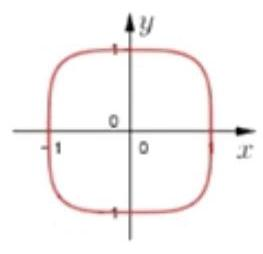
\includegraphics[max width=0.2\textwidth]{images/bo_d6dcisv7aajc739b5agg_136_352_1300_263_254_0.jpg}
\end{center}
\hspace*{3em} 

B.

\begin{center}
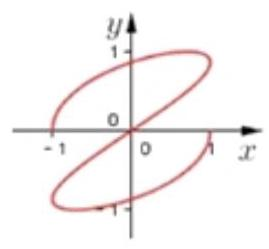
\includegraphics[max width=0.2\textwidth]{images/bo_d6dcisv7aajc739b5agg_136_950_1306_269_249_0.jpg}
\end{center}
\hspace*{3em} 

C.

\begin{center}
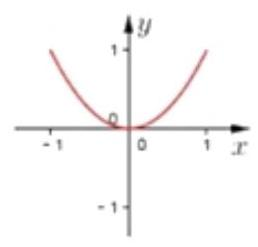
\includegraphics[max width=0.2\textwidth]{images/bo_d6dcisv7aajc739b5agg_136_370_1583_258_247_0.jpg}
\end{center}
\hspace*{3em} 

D.

\begin{center}
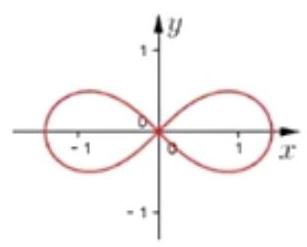
\includegraphics[max width=0.2\textwidth]{images/bo_d6dcisv7aajc739b5agg_136_948_1580_307_247_0.jpg}
\end{center}
\hspace*{3em} 

15. 已知 \(f\left( x\right)  = 3\sin x + 2\) ,对任意的 \({x}_{1} \in  \left\lbrack  {0,\frac{\pi }{2}}\right\rbrack\) ,都存在 \({x}_{2} \in  \left\lbrack  {0,\frac{\pi }{2}}\right\rbrack\) ,使得 \(f\left( {x}_{1}\right)  = {2f}\left( {{x}_{2} + \theta }\right) \; + 2\) 成立,则下列选项中, \(\theta\) 可能的值为 ( )

A. \(\frac{3\pi }{5}\) B. \(\frac{4\pi }{5}\) C. \(\frac{6\pi }{5}\) D. \(\frac{7\pi }{5}\)

16. 已知实数 \({x}_{1}\text{ 、 }{y}_{1}\text{ 、 }{x}_{2}\text{ 、 }{y}_{2}\text{ 、 }{x}_{3}\text{ 、 }{y}_{3}\) 为同时满足:  \circled{1}  \({x}_{1} < {y}_{1}\text{ ， }{x}_{2} < {y}_{2}\text{ ， }{x}_{3} < {y}_{3}\) ;  \circled{2}  \({x}_{1} + {y}_{1} = \; {x}_{2} + {y}_{2} = {x}_{3} + {y}_{3}\) ;  \circled{3}  \({x}_{1}{y}_{1} + {x}_{3}{y}_{3} = 2{x}_{2}{y}_{2}\) ,则下列选项恒成立的是 ( )

A. \(2{x}_{2} < {x}_{1} + {x}_{3}\) B. \(2{x}_{2} > {x}_{1} + {x}_{3}\) C. \({x}_{2}^{2} < {x}_{1}{x}_{3}\) D. \({x}_{2}^{2} > {x}_{1}{x}_{3}\)

\section*{三、解答题 (本大题共 5 题，共 \({14} + {14} + {14} + {16} + {18} = {76}\) 分)}

17. 如图，在长方体 \({ABCD} - {A}_{1}{B}_{1}{C}_{1}{D}_{1}\) ，已知 \({AB} = {BC} = 2\) ， \({A{A}_{1}} = 3\) .

\begin{center}
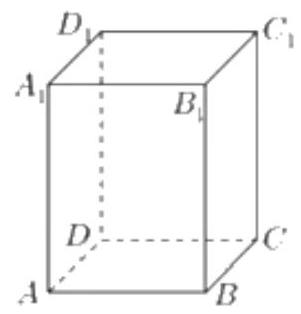
\includegraphics[max width=0.2\textwidth]{images/bo_d6dcisv7aajc739b5agg_137_265_1220_301_314_0.jpg}
\end{center}
\hspace*{3em} 

(1)若点 \(P\) 是棱 \({A}_{1}{D}_{1}\) 上的动点，求三棱锥 \(C - {PAD}\) 的体积；

18. 已知在 \({ABC}\) 中， \(A\) 、 \(B\) 、 \(C\) 所对边分别为 \(a\) 、 \(b\) 、 \(c\) ，且 \(a = 3\) ， \(b = {2c}\) .

(1)若 \(A = \frac{2\pi }{3}\) ，求 \({ABC}\) 的面积；

(2)若 \(2\sin B - \sin C = 1\) ，求 \({ABC}\) 的周长.

19. 已知某企业今年(2021年)第一季度的营业额为 1.1 亿元，以后每个季度的营业额比上个季度增加 0.05 亿元，该企业第一季度的利润为 0.16 亿，以后每季度比前一季度增长 4\%.

(1)求 2021 年起前 20 季度营业额的总和；

(2)请问哪一季度的利润首次超过该季度营业额的 18\%？

20. 已知椭圆 \(\Gamma  : \frac{{x}^{2}}{2} + {y}^{2} = 1,{F}_{1}\text{ 、 }{F}_{2}\) 是其左右焦点,直线 \(l\) 过点 \(P\left( {m,0}\right) \left( {m <  - \sqrt{2}}\right)\) 交椭圆 \(\Gamma\) 于 \(A\text{ 、 }B\) 两点,且 \(A\text{ 、 }B\) 在 \(x\) 轴上方,点 \(A\) 在线段 \({BP}\) 上.

(1)若 \(B\) 是上顶点， \(\left| \overrightarrow{B{F}_{1}}\right|  = \left| \overrightarrow{P{F}_{1}}\right|\) ，求 \(m\) 的值；

(2)若 \(\overrightarrow{{F}_{1}A} \cdot  \overrightarrow{{F}_{2}A} = {13}\) ，且原点 \(O\) 到直线 \(l\) 的距离为 \(\frac{4\sqrt{15}}{15}\) ，求直线 \(l\) 的方程；

(3)对于任意点 \(P\) ，是否存在唯一直线 \(l\) ，使得 \(\overrightarrow{{F}_{1}A}//\overrightarrow{{F}_{2}B}\) 成立，若存在，求出直线 \(l\) 的斜率，若不存在, 请说明理由.

21. 已知 \(f\left( x\right)\) 是定义在 \(R\) 上的函数,若对任意的 \({x}_{1}\text{ 、 }{x}_{2} \in  R,{x}_{1} - {x}_{2} \in  S\) ,均有 \(f\left( {x}_{1}\right)  - f\left( {x}_{2}\right) \; \in  S\) ,则称 \(f\left( x\right)\) 是 \(S\) 关联.

(1)判断和证明 \(f\left( x\right)  = {2x} + 1\) 是否是 \(\lbrack 0,\infty )\) 关联? 是否是 \(\left\lbrack  {0,1}\right\rbrack\) 关联?

(2)若 \(f\left( x\right)\) 是 \(\{ 3\}\) 关联，当 \(x \in  \lbrack 0,3)\) 时， \(f\left( x\right)  = {x}^{2} - {2x}\) ，解不等式 \(2 \leq  f\left( x\right)  \leq  3\) ；

(3)证明: “ \(f\left( x\right)\) 是 \(\{ 1\}\) 关联，且是 \(\lbrack 0, + \infty )\) 关联” 的充要条件是 “ \(f\left( x\right)\) 是 \(\left\lbrack  {1,2}\right\rbrack\) 关联” .

\section*{2021春考}

一、填空题(本大题共 12 题，满分 54 分，第 1\textasciitilde 6 题每题 4 分，第 7\textasciitilde 12 题每题 5 分) 1. 已知等差数列 \(\left\{  {a}_{n}\right\}\) 的首项为3，公差为2，则 \({a}_{10} =\) \_\_\_\_\_.

2. 已知 \(z = 1 - 3\mathrm{i}\) ，则 \(\left| {\bar{z} - \mathrm{i}}\right|  =\) \_\_\_\_\_.

3. 已知圆柱的底面半径为 1，母线长为 2，则该圆柱的侧面积等于\_\_\_\_\_.

4. 不等式 \(\frac{{2x} + 5}{x - 2} < 1\) 的解集为\_\_\_\_\_.

5. 直线 \(x =  - 2\) 与直线 \(\sqrt{3}x - y + 1 = 0\) 的夹角为\_\_\_\_\_.

6. 若方程组 \(\left\{  \begin{array}{l} {a}_{1}x + {b}_{1}y = {c}_{1} \\  {a}_{2}x + {b}_{2}y = {c}_{2} \end{array}\right.\) 无解,则 \(\left| \begin{array}{l} {a}_{1} \\  {a}_{2} \end{array}\right|  =\) \_\_\_\_\_.

7. 已知 \({\left( 1 + x\right) }^{n}\) 的展开式，唯有 \({x}^{3}\) 的系数最大，则 \({\left( 1 + x\right) }^{n}\) 的系数和为\_\_\_\_\_.

8. 已知函数 \(f\left( x\right)  = {3}^{x} + \frac{a}{{3}^{x} + 1}\left( {a0}\right)\) 的最小值为 5,则 \(a =\) \_\_\_\_\_.

9. 在无穷等比数列 \(\left\{  {a}_{n}\right\}\) 中， \(\mathop{\lim }\limits_{{n \rightarrow  \infty }}\left( {{a}_{1} - {a}_{n}}\right)  = 4\) ，则 \({a}_{2}\) 的取值范围是\_\_\_\_\_.

10. 某人某天需要运动总时长大于等于 60 分钟，现有五项运动可以选择，如表所示，问有几种运动方式组合\_\_\_\_\_.

\begin{center}
\adjustbox{max width=\textwidth}{
\begin{tabular}{|c|c|c|c|c|}
\hline
\(A\) 运动 & \(B\) 运动 & \(C\) 运动 & \(D\) 运动 & \(E\) 运动 \\
\cline{1-5}
\makecell{ 7 点 -8 \\ 点 } & \makecell{ 8 点 -9 \\ 点 } & \makecell{ 9 点 -10 \\ 点 } & \makecell{ 10 点 -11 \\ 点 } & \makecell{ 11 点 -12 \\ 点 } \\
\cline{1-5}
30 分钟 & 20 分钟 & 40 分钟 & 30 分钟 & 30 分钟 \\
\cline{1-5}
\hline
\end{tabular}
}
\end{center}

11. 已知椭圆 \({x}^{2} + \frac{{y}^{2}}{{b}^{2}} = 1\left( {0 < b < 1}\right)\) 的左、右焦点为 \({F}_{1}\text{ 、 }{F}_{2}\) ,以 \(O\) 为顶点， \({F}_{2}\) 为焦点作抛物线交椭圆于 \(P\) ，且 \(\angle P{F}_{1}{F}_{2} = {45}^{ \circ  }\) ，则抛物线的准线方程是\_\_\_\_\_.

12. 已知 \(\theta  > 0\) ,存在实数 \(\varphi\) ,使得对任意 \(n \in  {N}^{ * },\cos \left( {{n\theta } + \varphi }\right)  < \frac{\sqrt{3}}{2}\) ,则 \(\theta\) 的最小值是\_\_\_\_\_.

\section*{二、选择题 (本大题共 4 题, 每题 5 分, 共 20 分)}

13. 下列函数中, 在定义域内存在反函数的是 ( )

A. \(f\left( x\right)  = {x}^{2}\) B. \(f\left( x\right)  = \sin x\) C. \(f\left( x\right)  = {2x}\) D. \(f\left( x\right)  = 1\)

14. 已知集合 \(A = \{ x \mid  x - 1,x \in  R\} ,B = \left\{  {x \mid  {x}^{2} - x - 2 \geq  0,x \in  R}\right\}\) ，则下列关系中，正确的是 ( )

A. \(A \subseteq  B\) B. \({\complement }_{R}A \subseteq  {\complement }_{R}B\) C. \(A \cap  B = \varphi\) D. \(A \cup  B = R\)

15. 已知函数 \(y = f\left( x\right)\) 的定义域为 \(R\) ,下列是 \(f\left( x\right)\) 无最大值的充分条件是(   )

A. \(f\left( x\right)\) 为偶函数且关于点 \(\left( {1,1}\right)\) 对称 B. \(f\left( x\right)\) 为偶函数且关于直线 \(x = 1\) 对称

C. \(f\left( x\right)\) 为奇函数且关于点 \(\left( {1,1}\right)\) 对称 D. \(f\left( x\right)\) 为奇函数且关于直线 \(x = 1\) 对称

16. 在 \({ABC}\) 中， \(D\) 为 \({BC}\) 中点， \(E\) 为 \({AD}\) 中点，则以下结论: \circled{1} 存在 \({ABC}\) ，使得 \(\overrightarrow{AB} \cdot  \overrightarrow{CE} =\) 0 ;  \circled{2} 存在三角形 \({ABC}\) ，使得 \(\overrightarrow{CE}//\left( {\overrightarrow{CB} + \overrightarrow{CA}}\right)\) ；他们的成立情况是 ( )

A.  \circled{1} 成立， \circled{2} 不成立 B.  \circled{1} 成立， \circled{2} 不成立

C.  \circled{1} 不成立， \circled{2} 成立 D.  \circled{1} 不成立， \circled{2} 不成立

三、解答题 (本大题共 5 题, 共 \({14} + {14} + {14} + {16} + {18} = {76}\) 分)

17. 四棱锥 \(P - {ABCD}\) ,底面为正方形 \({ABCD}\) ,边长为 \(4,E\) 为 \({AB}\) 中点, \({PE} \bot\) 平面 \({ABCD}\) .

\begin{center}
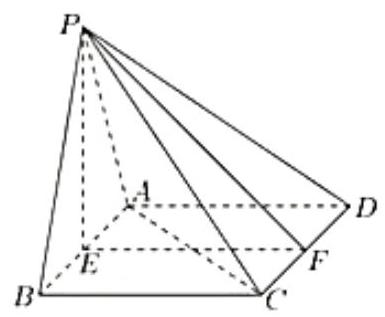
\includegraphics[max width=0.3\textwidth]{images/bo_d6dcisv7aajc739b5agg_142_282_469_385_317_0.jpg}
\end{center}
\hspace*{3em} 

(1)若 \({PAB}\) 为等边三角形，求四棱锥 \(P - {ABCD}\) 的体积；

(2)若 \({CD}\) 的中点为 \(F\) ， \({PF}\) 与平面 \({ABCD}\) 所成角为 \({45}^{ \circ  }\) ，求 \({PC}\) 与 \({AD}\) 所成角的大小.

18. 已知 \(A\text{ 、 }B\text{ 、 }C\) 为 \({ABC}\) 的三个内角， \(a\text{ 、 }b\text{ 、 }c\) 是其三条边， \(a = 2,\cos C =\) -14.

(1)若 \(\sin A = 2\sin B\) ,求 \(b\text{ 、 }c\) ;

( 2 )若 \(\cos \left( {A - \frac{\pi }{4}}\right)  = {45}\) ，求 \(c\) .

19. 完成下列试题

(1)团队在 \(O\) 点西侧、东侧 20 千米处设有 \(A\) 、 \(B\) 两站点，测量距离发现一点 \(P\) 满足 \(\left| {PA}\right| \; - \left| {PB}\right|  = {20}\) 千米,可知 \(P\) 在 \(A\text{ 、 }B\) 为焦点的双曲线上,以 \(O\) 点为原点,东侧为 \(x\) 轴正半轴, 北侧为 \(y\) 轴正半轴,建立平面直角坐标系, \(P\) 在北偏东 \({60}^{ \circ  }\) 处,求双曲线标准方程和 \(P\) 点坐标;

( 2 )团队又在南侧、北侧 15 千米处设有 \(C\) 、 \(D\) 两站点，测量距离发现 \(\left| {QA}\right|  - \left| {QB}\right|  = {30}\) 千米， \(\left| {QC}\right|  - \left| {QD}\right|  = {10}\) 千米,求 \(\left| {OQ}\right|\) (精确到 1 米) 和 \(Q\) 点位置 (精确到 1 米, \({1}^{ \circ  }\) ).

20. 已知函数 \(f\left( x\right)  = \sqrt{\left| {x + a}\right|  - a} - x\) .

(1)若 \(a = 1\) ，求函数的定义域；

(2)若 \(a \neq  0\) ，若 \(f\left( {ax}\right)  = a\) 有 2 个不同实数根，求 \(a\) 的取值范围；

(3) 是否存在实数 \(a\) ,使得函数 \(f\left( x\right)\) 在定义域内具有单调性? 若存在,求出 \(a\) 的取值范围.

21. 已知数列 \(\left\{  {a}_{n}\right\}\) 满足 \({a}_{n} \geq  0\) ,对任意 \(n \geq  2,{a}_{n}\) 和 \({a}_{n + 1}\) 中存在一项使其为另一项与 \({a}_{n - 1}\) 的等差中项.

(1)已知 \({a}_{1} = 5,{a}_{2} = 3,{a}_{4} = 2\) ，求 \({a}_{3}\) 的所有可能取值；

(2)已知 \({a}_{1} = {a}_{4} = {a}_{7} = 0,{a}_{2}\) 、 \({a}_{5}\) 、 \({a}_{8}\) 为正数，求证: \({a}_{2}\) 、 \({a}_{5}\) 、 \({a}_{8}\) 成等比数列，并求出公比 \(q\) ；

(3) 已知数列中恰有 3 项为 0，即 \({a}_{r} = {a}_{s} = {a}_{t} = 0,2 < r < s < t\) ，且 \({a}_{1} = 1,{a}_{2} = 2\) ，求 \({a}_{r + 1} + \; {a}_{s + 1} + {a}_{t + 1}\) 的最大值.

\section*{2022 秋考}

一、填空题(本大题共有 12 题，满分 54 分，第 1\textasciitilde 6 题每题 4 分，第 7\textasciitilde 12 题每题 5 分) 1. 已知 \(z = 1 + \mathrm{i}\) (其中 \(\mathrm{i}\) 为虚数单位),则 \(2\bar{z} =\) \_\_\_\_\_.

2. 双曲线 \(\frac{{x}^{2}}{9} - {y}^{2} = 1\) 的实轴长为\_\_\_\_\_.

3. 函数 \(f\left( x\right)  = {\cos }^{2}x - {\sin }^{2}x + 1\) 的最小正周期为\_\_\_\_\_.

4. \(= \frac{2\pi }{2} = \pi\) .

5. 已知 \(a \in  R\) ，行列式 \(\left| \begin{array}{l} a \\  3 \end{array}\right|\) 的值与行列式 \(\left| \begin{array}{l} a \\  4 \end{array}\right|\) 的值相等，则 \(a =\) \_\_\_\_\_.

6. 已知圆柱的高为4，底面积为9π，则圆柱的侧面积为\_\_\_\_\_.

7. \(x - y \leq  0,\;x + y - 1 \geq  0\) ,则 \(z = x + {2y}\) 的最小值为\_\_\_\_\_.

8. 二项式 \({\left( 3 + x\right) }^{n}\) 的展开式中, \({x}^{2}\) 项的系数是常数项的 5 倍,则 \(n =\) \_\_\_\_\_.

9. 若函数 \(f\left( x\right)  = \left\{  \begin{array}{l} {a}^{2}x - 1, \\  x + a, \\  0, \end{array}\right.\) ,为奇函数,则参数 \(a\) 的值为\_\_\_\_\_.

10. 为了检测学生的身体素质指标, 从游泳类 1 项, 球类 3 项, 田径类 4 项共 8 项项目中随机抽取 4 项进行检测, 则每一类都被抽到的概率为\_\_\_\_\_.

11. 已知等差数列 \(\left\{  {a}_{n}\right\}\) 的公差不为零, \({S}_{n}\) 为其前 \(n\) 项和,若 \({S}_{5} = 0\) ,则 \({S}_{i}\left( {\mathrm{i} = 1,2,\cdots ,{100}}\right)\) 中不同的数值有\_\_\_\_\_个。

12. 若平面向量 \(\left| \overrightarrow{a}\right|  = \left| \overrightarrow{b}\right|  = \left| \overrightarrow{c}\right|  = \lambda\) ，且满足 \(\overrightarrow{a} \cdot  \overrightarrow{b} = 0\) ， \(\overrightarrow{a} \cdot  \overrightarrow{c} = 2\) ， \(\overrightarrow{b} \cdot  \overrightarrow{c} = 1\) ，则 \(\lambda  =\) \_\_\_\_\_.

13. 设函数 \(f\left( x\right)\) 满足 \(f\left( x\right)  = f\left( \frac{1}{x + 1}\right)\) ,定义域为 \(D = \lbrack 0\) ， \(+ \infty )\) ，值域为 \(A\) ，若集合 \(\{ y \mid  y = f\left( x\right) \text{ ， }x \in  \left\lbrack  {0\text{ ， }a}\right\rbrack  \}\) 可取得 \(A\) 中所有值，则参数 \(a\) 的取值范围为\_\_\_\_\_.

二、选择题 (本题共有 4 题，满分 20 分，每题 5 分) 每题有且只有一个正确选项.

14. 若集合 \(A = \lbrack  - 1,2),B = Z\) ,则 \(A \cap  B =\) ( )

A. \(\{  - 2, - 1,0,1\}\) B. \(\{  - 1,0,1\}\)

C. \(\{  - 1,0\}\) D. \(\{  - 1\}\)

15. 若实数 \(a\text{ 、 }b\) 满足 \(a > b > 0\) ,下列不等式中恒成立的是 ( )

A. \(a + b > 2\sqrt{ab}\) B. \(a + b < 2\sqrt{ab}\) C. \(\frac{a}{2} + {2b} > 2\sqrt{ab}\) D. \(\frac{a}{2} + {2b} < 2\sqrt{ab}\)

16. 如图正方体 \({ABCD} - A{B}_{1}{C}_{1}{D}_{1}\) 中， \(P\) 、 \(Q\) 、 \(R\) 、 \(S\) 分别为棱 \({AB}\) 、 \({BC}\) 、 \(B{B}_{1}\) 、 \({CD}\) 的中点， 连接 \({A}_{1}S,{B}_{1}D\) . 空间任意两点 \(M\text{ 、 }N\) ,若线段 \({MN}\) 上不存在点在线段 \({A}_{1}S\text{ 、 }{B}_{1}D\) 上,则称 \({MN}\) 两点可视,则下列选项中与点 \({D}_{1}\) 可视的为( )

\begin{center}
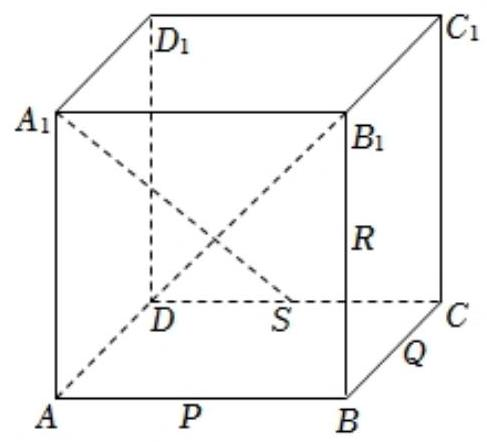
\includegraphics[max width=0.3\textwidth]{images/bo_d6dcisv7aajc739b5agg_147_263_234_487_442_0.jpg}
\end{center}
\hspace*{3em} 

A. 点 \(P\) B. 点 \(B\) C. 点 \(R\) D. 点 \(Q\)

17. 设集合 \(\Omega  = \left\{  {\left( {x,y}\right) \left| {{\left( x - k\right) }^{2} + {\left( y - {k}^{2}\right) }^{2} = 4}\right| k \mid  ,\;k \in  Z}\right\}\)

 \circled{1} 存在直线 \(l\) ，使得集合 \(\Omega\) 中不存在点在 \(l\) 上，而存在点在 \(l\) 两侧；

 \circled{2} 存在直线 \(l\) ，使得集合 \(\Omega\) 中存在无数点在 \(l\) 上； ( )

A.  \circled{1} 成立 \circled{2} 成立 B.  \circled{1} 成立 \circled{2} 不成立

C.  \circled{1} 不成立 \circled{2} 成立 D.  \circled{1} 不成立 \circled{2} 不成立

三、解答题 (本大题共有 5 题, 满分 76 分).

18. 如图所示三棱锥,底面为等边 \({\Delta ABC},O\) 为 \({AC}\) 边中点,且 \({PO} \bot\) 底面 \({ABC},{AP} = {AC} \; = 2\) .

\begin{center}
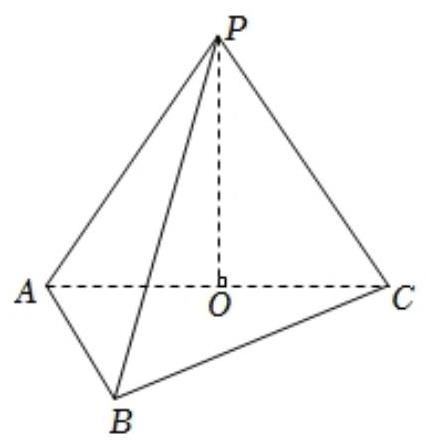
\includegraphics[max width=0.3\textwidth]{images/bo_d6dcisv7aajc739b5agg_147_297_1631_426_443_0.jpg}
\end{center}
\hspace*{3em} 

(1)求三棱锥体积 \({V}_{P - {ABC}}\) ；

(2)若 \(M\) 为 \({BC}\) 中点，求 \({PM}\) 与面 \({PAC}\) 所成角大小.

19. \(f\left( x\right)  = {\log }_{3}\left( {a + x}\right)  + {\log }_{3}\left( {6 - x}\right)\) .

(1)若将函数 \(f\left( x\right)\) 图像向下移 \(m\left( {m0}\right)\) 后，图像经过 \(\left( {3,0}\right)\) ， \(\left( {5,0}\right)\) ，求实数 \(a\) ， \(m\) 的值.

(2)若 \(a >  - 3\) 且 \(a \neq  0\) ，求解不等式 \(f\left( x\right)  \leq  f\left( {6 - x}\right)\) .

20. 在如图所示的图形中， \({AD} = {BC} = 6,{AB} = {20},O\) 为 \({AB}\) 中点，曲线 \({CD}\) 上任一点到 \(O\) 距离相等，角 \(\angle {DAB} = \angle {ABC} = {120}^{ \circ  }\) ， \(P\) ， \(Q\) 关于 \({OM}\) 对称， \({MO} \bot  {AB}\) ；

\begin{center}
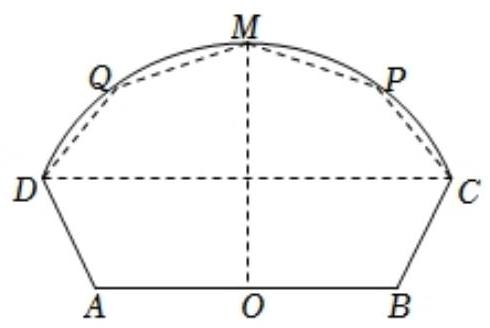
\includegraphics[max width=0.3\textwidth]{images/bo_d6dcisv7aajc739b5agg_148_283_1049_490_328_0.jpg}
\end{center}
\hspace*{3em} 

(1)若点 \(P\) 与点 \(C\) 重合，求 \(\angle {POB}\) 的大小；

(2)点 \(P\) 在何位置时，五边形 \({MQABP}\) 的面积最大，并求出该最大值.

21. 设有椭圆方程 \(\Gamma  : \frac{{x}^{2}}{{a}^{2}} + \frac{{y}^{2}}{{b}^{2}} = 1\left( {{ab} > 0}\right)\) ,直线 \(l : x + y - 4\sqrt{2} = 0,\Gamma\) 下端点为 \(A,M\) 在 \(l\) 上,左、右焦点分别为 \({F}_{1}\left( {-\sqrt{2},0}\right) \text{ 、 }{F}_{2}\left( {\sqrt{2},0}\right)\) .

(1) \(a = 2\) ， \({AM}\) 中点在 \(x\) 轴上，求点 \(M\) 的坐标；

(2) 直线 \(l\) 与 \(y\) 轴交于 \(B\) ,直线 \({AM}\) 经过右焦点 \({F}_{2}\) ,在 \(\bigtriangleup {ABM}\) 中有一内角余弦值为 \(\frac{3}{5}\) ,求 \(b\) ;

(3)在椭圆 \(\Gamma\) 上存在一点 \(P\) 到 \(l\) 距离为 \(d\) ，使 \(\left| {P{F}_{1}}\right|  + \left| {P{F}_{2}}\right|  + d = 6\) ，随 \(a\) 的变化，求 \(d\) 的最小值.

22. 数列 \(\left\{  {a}_{n}\right\}\) 对任意 \(n \in  {N}^{ * }\) 且 \(n \geq  2\) ,均存在正整数 \(\mathrm{i} \in  \left\lbrack  {1,n - 1}\right\rbrack\) ,满足 \({a}_{n + 1} = 2{a}_{n} - {a}_{i},{a}_{1} =\) 1, \({a}_{2} = 3\) .

(1)求 \({a}_{4}\) 可能值；

(2) 命题 \(p\) : 若 \({a}_{1},{a}_{2},\cdots ,{a}_{8}\) 成等差数列,则 \({a}_{9} < {30}\) ,证明 \(p\) 为真,同时写出 \(p\) 逆命题 \(q\) , 并判断命题 \(q\) 是真是假,说明理由;

(3)若 \({a}_{2m} = {3}^{m},\left( {m \in  {N}^{ * }}\right)\) 成立，求数列 \(\left\{  {a}_{n}\right\}\) 的通项公式.

\section*{2022 春考}

一、填空题(本大题共有 12 题，满分 54 分，第 1\textasciitilde 6 题每题 4 分，第 7\textasciitilde 12 题每题 5 分)

1. 已知 \(z = 2 + \mathrm{i}\) (其中 \(\mathrm{i}\) 为虚数单位),则 \(\bar{z} =\) \_\_\_\_\_.

2. 已知集合 \(A = \left( {-1,2}\right)\) ，集合 \(B = \left( {1,3}\right)\) ，则 \(A \cap  B =\) \_\_\_\_\_.

3. 不等式 \(\frac{x - 1}{x} < 0\) 的解集为\_\_\_\_\_.

4. 若 \(\tan \alpha  = 3\) ，则 \(\tan \left( {\alpha  + \frac{\pi }{4}}\right)  =\) \_\_\_\_\_.

5. 设函数 \(f\left( x\right)  = {x}^{3}\) 的反函数为 \({f}^{-1}\left( x\right)\) ，则 \({f}^{-1}\left( {27}\right)  =\) \_\_\_\_\_.

6. 在 \({\left( {x}^{3} + \frac{1}{x}\right) }^{12}\) 的展开式中，则含 \(\frac{1}{{x}^{4}}\) 项的系数为\_\_\_\_\_.

7. 若关于 \(x,y\) 的方程组 \(\left\{  \begin{array}{l} x + {my} = 2 \\  {mx} + {16y} = 8 \end{array}\right.\) 有无穷多解,则实数 \(m\) 的值为\_\_\_\_\_.

8. 已知在 \(\bigtriangleup {ABC}\) 中， \(\angle A = \frac{\pi }{3}\) ， \({AB} = 2\) ， \({AC} = 3\) ，则 \(\bigtriangleup {ABC}\) 的外接圆半径为\_\_\_\_\_.

9. 用数字 1、2、3、4 组成没有重复数字的四位数，则这些四位数中比 2134 大的数字个数为\_\_\_\_\_. (用数字作答)

10. 在 \(\bigtriangleup {ABC}\) 中, \(\angle A = {90}^{ \circ  },{AB} = {AC} = 2\) ,点 \(M\) 为边 \({AB}\) 的中点,点 \(P\) 在边 \({BC}\) 上,则 \(\overrightarrow{MP} \; \cdot  \overrightarrow{CP}\) 的最小值为\_\_\_\_\_.

11. 已知 \({P}_{1}\left( {{x}_{1},{y}_{1}}\right) ,{P}_{2}\left( {{x}_{2},{y}_{2}}\right)\) 两点均在双曲线 \(\Gamma  : \frac{{x}^{2}}{{a}^{2}} - {y}^{2} = 1\left( {a0}\right)\) 的右支上,若 \({x}_{1}{x}_{2} > {y}_{1}{y}_{2}\) 恒成立，则实数 \(a\) 的取值范围为\_\_\_\_\_.

12. 已知函数 \(y = f\left( x\right)\) 为定义域为 \(R\) 的奇函数,其图像关于 \(x = 1\) 对称,且当 \(x \in  (0,1\rbrack\) 时, \(f\left( x\right)  = \ln x\) ,若将方程 \(f\left( x\right)  = x + 1\) 的正实数根从小到大依次记为 \({x}_{1},{x}_{2},{x}_{3},\cdots ,{x}_{n}\) , 则 \(\mathop{\lim }\limits_{{n \rightarrow  \infty }}\left( {{x}_{n + 1} - {x}_{n}}\right)  =\) \_\_\_\_\_.

\section*{二、选择题 (本大题共有 4 题, 满分 20 分, 每题 5 分) 每题有且只有一个正确选项, 考生 应在答题纸的相应位置, 将代表正确选项的小方格涂黑.}

13. 下列函数定义域为 \(R\) 的是 ( ).

A. \(y = {x}^{-\frac{1}{2}}\) B. \(y = {x}^{-1}\) C. \(y = {x}^{\frac{1}{3}}\) D. \(y = {x}^{\frac{1}{2}}\)

14. 若 \(a > b > c > d\) ,则下列不等式恒成立的是 ( ).

A. \(a + d > b + c\) B. \(a + c > b + d\) C. \({ac} > {bd}\) D. \({ad} > {bc}\)

15. 上海海关大楼的顶部为逐级收拢的四面钟楼, 如图, 四个大钟分布在四棱柱的四个侧面, 则每天 0 点至 12 点 (包含 0 点,不含 12 点) 相邻两钟面上的时针相互垂直的次数为().

\begin{center}
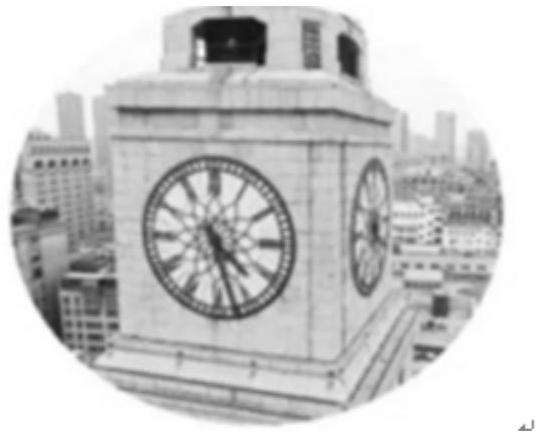
\includegraphics[max width=0.4\textwidth]{images/bo_d6dcisv7aajc739b5agg_152_287_1359_542_434_0.jpg}
\end{center}
\hspace*{3em} 

A. 0 B. 2 C. 4 D. 12

16. 已知等比数列 \(\left\{  {a}_{n}\right\}\) 的前 \(n\) 项和为 \({S}_{n}\) ,前 \(n\) 项积为 \({T}_{n}\) ,则下列选项判断正确的是 ( ).

A. 若 \({S}_{2022} > {S}_{2021}\) ,则数列 \(\left\{  {a}_{n}\right\}\) 是递增数列

B. 若 \({T}_{2022} > {T}_{2021}\) ,则数列 \(\left\{  {a}_{n}\right\}\) 是递增数列

C. 若数列 \(\left\{  {S}_{n}\right\}\) 是递增数列,则 \({a}_{2022} \geq  {a}_{2021}\)

D. 若数列 \(\left\{  {T}_{n}\right\}\) 是递增数列,则 \({a}_{2022} \geq  {a}_{2021}\)

三、简答题 (本大题共有 5 题, 满分 76 分) 解答下列各题必须在答题纸的相应位置写出必要的步骤.

17. 如图,圆柱下底面与上底面的圆心分别为 \(O\text{ 、 }{O}_{1},A{A}_{1}\) 为圆柱的母线,底面半径长为 1 .

\begin{center}
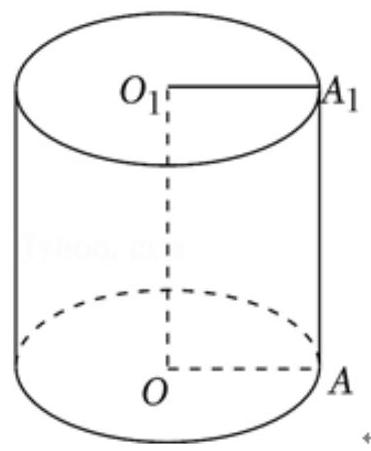
\includegraphics[max width=0.2\textwidth]{images/bo_d6dcisv7aajc739b5agg_153_291_916_371_451_0.jpg}
\end{center}
\hspace*{3em} 

(1)若 \(A{A}_{1} = 4,{M\;\text{ 为 }\;A{A}_{1}}\) 的中点，求直线 \(M{O}_{1}\) 与上底面所成角的大小；(结果用反三角函数值表示)

(2)若圆柱过 \(O{O}_{1}\) 的截面为正方形，求圆柱的体积与侧面积.

18. 已知在数列 \(\left\{  {a}_{n}\right\}\) 中, \({a}_{2} = 1\) ,其前 \(n\) 项和为 \({S}_{n}\) .

(1)若 \(\left\{  {a}_{n}\right\}\) 是等比数列， \({S}_{2} = 3\) ，求 \(\mathop{\lim }\limits_{{n \rightarrow  \infty }}{S}_{n}\) ；

(2)若 \(\left\{  {a}_{n}\right\}\) 是等差数列， \({S}_{2n} \geq  n\) ，求其公差 \(d\) 的取值范围.

19. 为有效塑造城市景观、提升城市环境品质，上海市正在努力推进新一轮架空线入地工程的建设. 如图是一处要架空线入地的矩形地块 \({ABCD},{AB} = {30m},{AD} = {15m}\) . 为保护 \(D\) 处的一棵古树,有关部门划定了以 \(D\) 为圆心、 \({DA}\) 为半径的四分之一圆的地块为历史古迹封闭区. 若空线入线口为 \({AB}\) 边上的点 \(E\) ,出线口为 \({CD}\) 边上的点 \(F\) ,施工要求 \({EF}\) 与封闭区边界相切, \({EF}\) 右侧的四边形地块 \({BCFE}\) 将作为绿地保护生态区. (计算长度精确到 \({0.1}\mathrm{\;m}\) ,计算面积精确到 \({0.01}{\mathrm{\;m}}^{2}\) )

\begin{center}
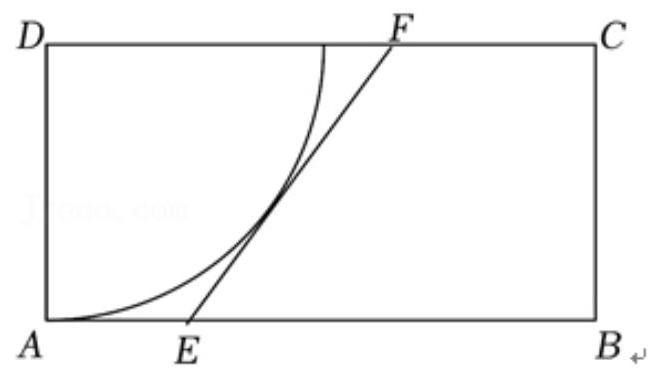
\includegraphics[max width=0.5\textwidth]{images/bo_d6dcisv7aajc739b5agg_154_265_512_653_373_0.jpg}
\end{center}
\hspace*{3em} 

(1)若 \(\angle {ADE} = {20}^{ \circ  }\) ，求 \({EF}\) 的长；

(2)当入线口 \(E\) 在 \({AB}\) 上的什么位置时，生态区的面积最大？最大面积是多少？

20. 已知椭圆 \(\Gamma  : \frac{{x}^{2}}{{a}^{2}} + {y}^{2} = 1\left( {a1}\right) ,A\text{ 、 }B\) 两点分别为 \(\Gamma\) 的左顶点、下顶点, \(C\text{ 、 }D\) 两点均在直线 \(l : x = a\) 上,且 \(C\) 在第一象限.

(1)设 \(F\) 是椭圆 \(\Gamma\) 的右焦点，且 \(\angle {AFB} = \frac{\pi }{6}\) ，求 \(\Gamma\) 的标准方程；

(2)若 \(C\) 、 \(D\) 两点纵坐标分别为2、1，请判断直线 \({AD}\) 与直线 \({BC}\) 的交点是否在椭圆 \(\Gamma\) 上，并说明理由;

(3) 设直线 \({AD}\text{ 、 }{BC}\) 分别交椭圆 \(\Gamma\) 于点 \(P\) 、点 \(Q\) ，若 \(P\text{ 、 }Q\) 关于原点对称，求 \(\left| {CD}\right|\) 的最小值.

21. 已知函数 \(f\left( x\right)\) 的定义域为 \(R\) ,现有两种对 \(f\left( x\right)\) 变换的操作: \(\varphi\) 变换: \(f\left( x\right)  - f\left( {x - t}\right)\) ； 变换: \(\left| {f\left( {x + t}\right)  - f\left( x\right) }\right|\) ，其中 \(t\) 为大于 0 的常数.

(1) 设 \(f\left( x\right)  = {2}^{x},t = 1,g\left( x\right)\) 为 \(f\left( x\right)\) 做 \(\varphi\) 变换后的结果，解方程: \(g\left( x\right)  = 2\) ；

(2)设 \(f\left( x\right)  = {x}^{2},h\left( x\right)\) 为 \(f\left( x\right)\) 做 \(\omega\) 变换后的结果，解不等式: \(f\left( x\right)  \geq  h\left( x\right)\) ；

(3) 设 \(f\left( x\right)\) 在 \(\left( {-\infty ,0}\right)\) 上单调递增, \(f\left( x\right)\) 先做 \(\varphi\) 变换后得到 \(u\left( x\right) ,u\left( x\right)\) 再做 \(\omega\) 变换后得到

\({h}_{1}\left( x\right) ;f\left( x\right)\) 先做 \(\omega\) 变换后得到 \(v\left( x\right) ,v\left( x\right)\) 再做 \(\varphi\) 变换后得到 \({h}_{2}\left( x\right)\) . 若 \({h}_{1}\left( x\right)  = {h}_{2}\left( x\right)\) 恒成立, 证明: 函数 \(f\left( x\right)\) 在 \(R\) 上单调递增.
\end{document}